\documentclass[]{article}
\usepackage{lmodern}
\usepackage{amssymb,amsmath}
\usepackage{ifxetex,ifluatex}
\usepackage{fixltx2e} % provides \textsubscript
\ifnum 0\ifxetex 1\fi\ifluatex 1\fi=0 % if pdftex
  \usepackage[T1]{fontenc}
  \usepackage[utf8]{inputenc}
\else % if luatex or xelatex
  \ifxetex
    \usepackage{mathspec}
  \else
    \usepackage{fontspec}
  \fi
  \defaultfontfeatures{Ligatures=TeX,Scale=MatchLowercase}
\fi
% use upquote if available, for straight quotes in verbatim environments
\IfFileExists{upquote.sty}{\usepackage{upquote}}{}
% use microtype if available
\IfFileExists{microtype.sty}{%
\usepackage{microtype}
\UseMicrotypeSet[protrusion]{basicmath} % disable protrusion for tt fonts
}{}
\usepackage[margin=1in]{geometry}
\usepackage{hyperref}
\hypersetup{unicode=true,
            pdfborder={0 0 0},
            breaklinks=true}
\urlstyle{same}  % don't use monospace font for urls
\usepackage{color}
\usepackage{fancyvrb}
\newcommand{\VerbBar}{|}
\newcommand{\VERB}{\Verb[commandchars=\\\{\}]}
\DefineVerbatimEnvironment{Highlighting}{Verbatim}{commandchars=\\\{\}}
% Add ',fontsize=\small' for more characters per line
\usepackage{framed}
\definecolor{shadecolor}{RGB}{248,248,248}
\newenvironment{Shaded}{\begin{snugshade}}{\end{snugshade}}
\newcommand{\AlertTok}[1]{\textcolor[rgb]{0.94,0.16,0.16}{#1}}
\newcommand{\AnnotationTok}[1]{\textcolor[rgb]{0.56,0.35,0.01}{\textbf{\textit{#1}}}}
\newcommand{\AttributeTok}[1]{\textcolor[rgb]{0.77,0.63,0.00}{#1}}
\newcommand{\BaseNTok}[1]{\textcolor[rgb]{0.00,0.00,0.81}{#1}}
\newcommand{\BuiltInTok}[1]{#1}
\newcommand{\CharTok}[1]{\textcolor[rgb]{0.31,0.60,0.02}{#1}}
\newcommand{\CommentTok}[1]{\textcolor[rgb]{0.56,0.35,0.01}{\textit{#1}}}
\newcommand{\CommentVarTok}[1]{\textcolor[rgb]{0.56,0.35,0.01}{\textbf{\textit{#1}}}}
\newcommand{\ConstantTok}[1]{\textcolor[rgb]{0.00,0.00,0.00}{#1}}
\newcommand{\ControlFlowTok}[1]{\textcolor[rgb]{0.13,0.29,0.53}{\textbf{#1}}}
\newcommand{\DataTypeTok}[1]{\textcolor[rgb]{0.13,0.29,0.53}{#1}}
\newcommand{\DecValTok}[1]{\textcolor[rgb]{0.00,0.00,0.81}{#1}}
\newcommand{\DocumentationTok}[1]{\textcolor[rgb]{0.56,0.35,0.01}{\textbf{\textit{#1}}}}
\newcommand{\ErrorTok}[1]{\textcolor[rgb]{0.64,0.00,0.00}{\textbf{#1}}}
\newcommand{\ExtensionTok}[1]{#1}
\newcommand{\FloatTok}[1]{\textcolor[rgb]{0.00,0.00,0.81}{#1}}
\newcommand{\FunctionTok}[1]{\textcolor[rgb]{0.00,0.00,0.00}{#1}}
\newcommand{\ImportTok}[1]{#1}
\newcommand{\InformationTok}[1]{\textcolor[rgb]{0.56,0.35,0.01}{\textbf{\textit{#1}}}}
\newcommand{\KeywordTok}[1]{\textcolor[rgb]{0.13,0.29,0.53}{\textbf{#1}}}
\newcommand{\NormalTok}[1]{#1}
\newcommand{\OperatorTok}[1]{\textcolor[rgb]{0.81,0.36,0.00}{\textbf{#1}}}
\newcommand{\OtherTok}[1]{\textcolor[rgb]{0.56,0.35,0.01}{#1}}
\newcommand{\PreprocessorTok}[1]{\textcolor[rgb]{0.56,0.35,0.01}{\textit{#1}}}
\newcommand{\RegionMarkerTok}[1]{#1}
\newcommand{\SpecialCharTok}[1]{\textcolor[rgb]{0.00,0.00,0.00}{#1}}
\newcommand{\SpecialStringTok}[1]{\textcolor[rgb]{0.31,0.60,0.02}{#1}}
\newcommand{\StringTok}[1]{\textcolor[rgb]{0.31,0.60,0.02}{#1}}
\newcommand{\VariableTok}[1]{\textcolor[rgb]{0.00,0.00,0.00}{#1}}
\newcommand{\VerbatimStringTok}[1]{\textcolor[rgb]{0.31,0.60,0.02}{#1}}
\newcommand{\WarningTok}[1]{\textcolor[rgb]{0.56,0.35,0.01}{\textbf{\textit{#1}}}}
\usepackage{graphicx,grffile}
\makeatletter
\def\maxwidth{\ifdim\Gin@nat@width>\linewidth\linewidth\else\Gin@nat@width\fi}
\def\maxheight{\ifdim\Gin@nat@height>\textheight\textheight\else\Gin@nat@height\fi}
\makeatother
% Scale images if necessary, so that they will not overflow the page
% margins by default, and it is still possible to overwrite the defaults
% using explicit options in \includegraphics[width, height, ...]{}
\setkeys{Gin}{width=\maxwidth,height=\maxheight,keepaspectratio}
\IfFileExists{parskip.sty}{%
\usepackage{parskip}
}{% else
\setlength{\parindent}{0pt}
\setlength{\parskip}{6pt plus 2pt minus 1pt}
}
\setlength{\emergencystretch}{3em}  % prevent overfull lines
\providecommand{\tightlist}{%
  \setlength{\itemsep}{0pt}\setlength{\parskip}{0pt}}
\setcounter{secnumdepth}{0}
% Redefines (sub)paragraphs to behave more like sections
\ifx\paragraph\undefined\else
\let\oldparagraph\paragraph
\renewcommand{\paragraph}[1]{\oldparagraph{#1}\mbox{}}
\fi
\ifx\subparagraph\undefined\else
\let\oldsubparagraph\subparagraph
\renewcommand{\subparagraph}[1]{\oldsubparagraph{#1}\mbox{}}
\fi

%%% Use protect on footnotes to avoid problems with footnotes in titles
\let\rmarkdownfootnote\footnote%
\def\footnote{\protect\rmarkdownfootnote}

%%% Change title format to be more compact
\usepackage{titling}

% Create subtitle command for use in maketitle
\providecommand{\subtitle}[1]{
  \posttitle{
    \begin{center}\large#1\end{center}
    }
}

\setlength{\droptitle}{-2em}

  \title{}
    \pretitle{\vspace{\droptitle}}
  \posttitle{}
    \author{}
    \preauthor{}\postauthor{}
    \date{}
    \predate{}\postdate{}
  

\begin{document}

\doublespacing

\section{Introduction}
\label{sec3:Introduction}

The fundamental premise in the nature behind ORMFs, is to provide an
exposure-based treatment of OpRisk losses which caters to modeling
capital estimates for forward-looking aspects of ORM. This proves tricky
as a requirement, due to the need for specific knowledge about potential
loss events, from the time the loss event occurs and the underlying
loss-generating mechanisms, until the actual realised loss materialises.
By its very nature, OpRisk is characterised by a significant lag between
the moment the event is conceived to the point the event is observed and
accounted for.\medskip 

For example, in the case of rogue trading, there is a frequency exposure
associated with traders \emph{going rogue}, due to a probability of
rogue events happening between a specific group of traders over time,
which is then modeled for each rogue trading event and the impact
(severity based on the size of the position) of the loss when it is
realised (at time of detection). This timing paradox often results in
questionable capital estimates, especially for those near misses,
pending and realised losses that need to be captured in the model.

\section{Applicability of EBOR methodology for capturing forward-looking aspects of ORM}
\label{sec:Applicability of EBOR methodology for capturing forward-looking aspects of ORM}

OpRisk is characterised by a time delay \(\tau\), wherein the p\&l
impact lags behind the moment the OpRisk event is conceived up until the
event is observed and accounted for. Advancing our knowledge toward the
current ORMF's aims to provide an exposure-based treatment of OpRisk
losses which caters for modeling capital estimates of forward-looking
aspects of ORM.\medskip

@einemann2018operational unearth a useful EBOR model, wherein an
additional cell is considered, anagolous to the BL/ET matrix
combinations, contributing into the classical LDA model thereby building
hybrid OpRisk frameworks which integrate EBOR models with the LDA model,
facilitating the migration of OpRisk types from a classical to an
exposure-based treatment through a quantitative framework
{[}@einemann2018operational{]}. Conceptually, the EBOR model component
can be extended to include potential future events e.g., future
litigations, based on some underlying property, capturing forward
looking aspects of business environment and internal control factors
(BEICF's) thereof.\medskip

The fundamental premise behind the LDA is that each firm's OpRisk losses
are a reflection of it's underlying OpRisk exposure
{[}@einemann2018operational{]}. @dobson2008introduction relates OpRisk
events to a varying or a constant degree of exposure, which needs to be
taken into account when modeling counts or frequencies of occurance. In
particular, the assumption behind the use of the Poisson distribution in
the model to estimate the frequency of losses for all available
observations, is that both the the intensity (or rate) of occurrence and
the opportunity (or exposure) for counting can assume either of these
two afore-mentioned forms {[}@dobson2008introduction{]}. In the former
case the varying degrees of exposure impact on the rate of events,
whereas in the latter case the exposure is constant hence not relevant
to the model.\medskip

When observed counts all have the same exposure, modeling the mean count
\(\mu\) as a function of explanatory variables \(x_{1},\ldots,x_{p}\) is
the same as modeling the rate \(R\). The actual measure of exposure we
need to use depends specifically on projecting the count of OpRisk
events (frequency of realised losses) as the target variable in the
model as opposed to the measure if the target variable were the severity
of the losses, e.g.~in modeling rogue trading severity exposure of
events is based on size of loss position at time to detection or
CapturedBy as severity risk factors.

\subsection{Definition of exposure}
\label{ssec:Definition of exposure}

Exposure is residual risk, or the risk that remains after risk
treatments have been applied. In the ORMF context, it is defined as:

\begin{definition}
The  \textbf{exposure} of risk type $i$, $d_{i}$ is the time interval, expressed in units of time, from the initial moment when the event happened, until the occurrence of a risk correction.
\end{definition}

As per definition \ref{ssec:Definition of exposure}, the lag represents
exposure; we need historical exposure for experience rating because we
need to be able to compare the loss experience of different years on a
like-for-like basis and to adjust it to current exposure levels
{[}@parodi2014pricing{]}.

\subsection{Definition of rate}
\label{ssec:Definition of rate}

Often the poisson count \(\lambda\) needs to be described as a rate; for
example the OpRisk hazard rate can be specified as the rate per day.
More generally, the rate is specified in terms of units of
\emph{exposure}; The \textbf{rate}, \(R\) is defined as:\medskip

\begin{definition}
the \textbf{rate} is the mean count per unit exposure
\end{definition}

i.e., \singlespacing \begin{eqnarray}
R &=& \frac{\mu}{\tau} \qquad \mbox{where} \qquad R = \mbox{rate,} \quad \tau = \mbox{exposure},d_{i}\quad \mbox{and}\nonumber\\
\mu &=& \mbox{mean count over an exposure duration of} \quad d = [T,T+\tau] \nonumber
\end{eqnarray} \doublespacing

For example, in OpRisk hazard rates, each potential OpRisk transaction
event is ``exposed'' over the period \([T,T+\tau]\); it's detection life
cycle period, and a P\&L impact determined, So the rate may be defined
in terms of transcaction-days \emph{at risk}.

\subsection{Limitations of the EBOR model}

In their model {[}@einemann2018operational{]}, the definition of
exposure, Definition \ref{ssec:Definition of exposure}, is particularly
well-suited to the specific risk type dealt with in their paper i.e.,
the portfolio of litigation events, due to better usage of existing
information and more plausible model behavior over the litigation life
cycle. However, it is bound to under-perform for many other OpRisk event
types since these EBOR models are typically designed to quantify
specific aspects of OpRisk i.e., litigation risk have rather
concentrated risk profiles. Furthermore, EBOR models are important due
to wide applicability beyond capital calculation and its potential to
evolve into an important tool for auditing process and early detection
of potential losses.

\section{Generalised Linear Models (GLM's)}
\label{sec:Generalised Linear Models}

Many of the ideas and concepts {[}@dobson2008introduction{]} of linear
modelling carry over to generalized linear modelling, however the
``generalized'' term is used to refer to all linear models other than
simple straight lines found in the ``general'' case. In the case of the
OpRisk dataset, the relationship between outcomes and drivers of risk
are frequently not normal, therefore models of the form

\singlespacing

\begin{eqnarray}\label{linearmodel}
E(\mathbf{Y_i}) = \mathbf{\mu_i} = \mathbf{x_i}^T\mathbf{\beta} \qquad \mathbf{Y_i} \thicksim \mathbf{N(\mu_i, \sigma^2)},
\end{eqnarray} \doublespacing

where random variables \(\mathbf{Y_i}\) are independent, are not
applicable. The transposed vector \(\mathbf{x_i}^T\) represents the
\(i\)th row of the dataset \(\mathbf{X}\). In such cases, due to recent
advances in statistical theory and computational techniques, generalised
linear models (GLM); which are analogous to linear models, are used to
assess and quantify the relationships between a target variable and
explanatory variables {[}@dobson2008introduction{]}. GLM's differ in
that

\begin{itemize}
\item The distribution of the target variable is chosen from the exponential family
\item A transformation of the mean of the response is linearly related to the explanatory variables, however their association need not be of the simple linear form in equation \ref{linearmodel}
\end{itemize}
\medskip

Operational riskiness in FIs grows as trading transactions grow in
complexity i.e., the more complex and numerous trading activity builds
the higher the rate at which new cases of OpRisk events occur.
Therefore, it is likely that the rate of operational hazard may be
increasing exponentially over time. The scientifically interesting
question is whether the data provides any evidence that the increase in
the underlying operational hazard generation is slowing. The
afore-mentioned postulate provides a plausible model to start
investigating this question.\medskip

\section{Exponential family of distributions}
\label{sec: Exponential family of distributions}

As with the linear model, consider independent rv's \(\mathbf{Y_i}\) not
i.i.d, whose probability depends on a parameter \(\theta_i\). The choice
of parameter \(\theta_i\) determines the response distribution which is
assumed to have the same form as the exponential family, in turn
characterising the statistical unit \(i\). Thus, the exponential family
representation depends on varying parameters \(\theta_i\), and a
constant scale parameter \(\phi\). the pdf of \(\mathbf{Y_i}\) is

\singlespacing

\begin{eqnarray}\label{Exponentialfamily}
f(y_i;\theta_i;\phi) = \exp\left[\frac{a(y_i)b(\theta_i) -c(\theta_i)}{\phi}-d(y_i,\phi)\right], \quad y_i \in Y 
\end{eqnarray} \doublespacing

where \(a\), \(b\), \(c\), \& \(d\) are regarded as known functions.
Expanding the expression in equation \ref{Exponentialfamily} yields

\singlespacing

\begin{eqnarray}\label{Exponentialfamilies}
f(y_i;\theta_i;\phi) &=& \exp\left[\frac{a(y_i)b(\theta_i) -c(\theta_i)}{\phi}-d(y_i,\phi)\right] \nonumber\\
 &=& \frac{1}{e^{d(y,\phi)}}\exp\left[\frac{a(y_i)b(\theta_i) -c(\theta_i)}{\phi}\right] \nonumber\\
 &=& r(y,\phi)\frac{1}{e^{\frac{c(\theta_i)}{\phi}}}\exp\left[\frac{a(y_i)b(\theta_i)}{\phi}\right] \nonumber\\
 &=& r(y,\phi)s(\theta,\phi)\exp\left[\frac{a(y_i)b(\theta_i)}{\phi}\right]\\
 \mbox{where} \quad r(y,\phi) &=& \frac{1}{e^{d(y,\phi)}}\quad \mbox{and where}\quad s(\theta,\phi) = \frac{1}{e^{\frac{c(\theta_i)}{\phi}}}\nonumber
\end{eqnarray} \doublespacing

since the scale parameter \(\phi\) is constant, the distribution belongs
to the exponential family if it can be written in the form

\singlespacing

\begin{eqnarray}\label{Exponential}
f(y;\theta) = r(y)s(\theta)\mathbf{e}^{a(y)b(\theta)}
\end{eqnarray} \doublespacing

If \(a(y) = y\), the distribution is in canonical form and \(b(\theta)\)
is called the natural parameter of the response distribution
{[}@de2008generalized{]}. The specific elements of a GLM are
{[}@dobson2008introduction; @covrig2015using{]}:

\begin{enumerate}
\item The random component given by the independent random variables $Y_1, Y_2, \ldots, Y_n $ not identically distributed. Note that the rv's $\mathbf{Y_i}$ for the Oprisk data, indexed by the subscript $i$, have different expected values $\mu_i$. Sometimes there may be only one observation $y_i$ for each $Y_i$, but there may be several observations $y_{ij}, (j=1,\ldots,n_i)$ for each $\mathbf{Y_i}$. The pdf or probability mass function of $\mathbf{Y_i}$ is given in equation \ref{Exponential} for $f(y)$, which specifies that the distribution of the response is in the exponential family. The support set $X$ of the rv $Y_i$ is subset of $\mathbf{N}$ of $\mathbf{R}$. 

\item The second advance is the extension of computational methods to estimate the models systematic component, so called the "linear predictor" described in equation \ref{linearmodel} built with $p+1$ parameters $\mathbf{\beta} = (\beta_0,\beta_1,\ldots,\beta_p)$ and with $p$ explanatory variables:

\singlespacing
\begin{eqnarray}\label{linearpredictor}
\eta_i = \beta_0 + \sum_{j=1}^{p}\beta_jx_{ij}, \qquad i = 1,2,\ldots,n
\end{eqnarray}
\doublespacing

\item The equation for $\eta_i$ specifies to the situation that there is some non-linear function, a transformation of the mean, $g(\mu)$, that is linearly related to the explanatory variables contained on the r.h.s of equation \ref{linearpredictor}, $\mathbf{X_i}^T\mathbf{\beta}$, i.e.,

\singlespacing
\begin{eqnarray}
g(\mu_i) = \mathbf{X_i}^T\mathbf{\beta}
\end{eqnarray}
\doublespacing

The function $g(\mu_i)$ is called the link function.
\end{enumerate}

\subsection{Interpretation}

Given a response variable \(y\), for the initial formulation of glm's by
@nelder1972generalized, \(b(\theta)\) determines the nature of the
response distribution and the choice of link is suggested by the
functional form of the relationship between the response and explanatory
variables. In choosing these components extra steps are taken compared
to ordinary regression modeling. Commonly used links functions are given
in Table \ref{tab_linkfcn} which also presents the units produced for
the various GLM links.

\begin{table}[tb]
\centering
\caption{The generalized linear model link functions with their associated units of interpretation. Note: This list is not exhaustive and there are likely more GLMs that are used within prevention research.} 
\label{tab_linkfcn}
\begin{tabular}{lcll}
\toprule
Link Function & $g(\mu)$ & Target variable Effect & Canonical link for \\ 
\midrule
Identity & $\mu$ & Original Continuous Unit & normal \\ 
  Log & ln$\mu$ & count & poisson \\ 
  Logit & ln $\frac{\mu}{1-\mu}$ & Risk & binomial \\ 
  Probit & $\phi^{-1}(\theta)$ & Risk & binomial \\ 
  Power & $\mu^p$ & Count & $\Gamma(p=-1)$\\
        &       & Count & inverse Gaussian(p=-2)\\
\bottomrule
\end{tabular}
\end{table}

\subsubsection{Offsets}

Modeling counts as realised operational hazard in an OpRisk group
requires correction for the period in days \(d\) exposed to risk. If
\(\mu\) is the mean of the count \(y\) then the occurence rate of
interest \(R= \frac{\mu}{d}\) and

\singlespacing

\begin{eqnarray}
g\left(\frac{\mu}{d}\right) = \mathbf{x}^T\mathbf{\beta}
\end{eqnarray} \doublespacing

When \(g\) is the log function, this becomes

\singlespacing

\begin{eqnarray}\label{offset}
\mbox{ln}\left(\frac{\mu}{d}\right) = \mathbf{x}^T\mathbf{\beta} \quad \Rightarrow \quad \mbox{ln}\mu = \mbox{ln}d + \mathbf{x}^T\mathbf{\beta}
\end{eqnarray} \doublespacing

Where the variable \(d\) appears representing the risk \emph{exposure}
and ln\(d\) is called an ``offset''. Equation \ref{offset} differs from
the usual specification of the linear predictor due to the inclusion of
the term ln\(d\). An offset is effectively another explanatory variable
in the regression, with a \(\beta\) coefficient = 1. With the offset,
\(y\) has expected value directly proportional to exposure:

\singlespacing

\begin{eqnarray}
E(Y) = \mu = d e^{x^T\beta}
\end{eqnarray} \doublespacing

Offsets are used to correct for differing periods of observation
{[}@de2008generalized{]} i.e., in the opRisk dataset these are the times
to detection (exposure) of the realised losses. The exposure measure is
a known constant which is readily incorporated into the estimation
procedure and is a quantity that is roughly proportional to the risk
{[}@parodi2014pricing{]} i.e., when the exposure (time to detection)
doubles whilst everthing else (e.g.~interest on an interest rate swap)
remains the same, the risk also doubles.

\section{Generalized linear model for count data}
\label{sec:Generalized linear model for count data}

\subsection{Exponential family of distributions}

Concluding Section \ref{sec:Generalised Linear Models} in Chapter
\ref{EXPOSURE-BASED OPERATIONAL RISK ANALYSIS}, the question of
increasing OpRisk hazard rates due to increasing transaction complexity
was raised, wherein \(\mu_i\), the expected number of new cases on day
\(t_i\) is modeled. The model assumes that the number of expected new
OpRisk hazards often increase exponentially over time. Hence, if
\(\mu_i\) is the expected number of new cases over time
\([T,T+\tau] = t_i\), then an appropraite model takes the form:

\singlespacing

\begin{eqnarray}\label{expgrowth}
E(\mathbf{Y}_i) = \mu_i = d_i\exp{(\beta t_i)} 
\end{eqnarray} \doublespacing

where the random variables \(\mathbf{Y_i}\) are independent,
\(d_i = \mbox{exposure}_i\), and \(\beta\)'s are a set of unknown
parameters in \(\mathbf{\beta}\). For a list of \(N\) different Oprisk
events, note that the random variables \(Y_i\) are the basis for the
OpRisk hazard defined by a binary response variable \emph{LossIndicator}
which denotes the presence or absence loss. Define random variabels
\(Y_1,\ldots,Y_N\) as follows

\begin{definition}\label{DefLosInd}
\singlespacing
\begin{equation}\label{LossIndicator}
\mathbf {Y}_i =\left\{\begin{array}{rcl}
                 & 1 & \mbox{for realised OpRisk losses}  \\
                 & 0 & \mbox{for pending losses and near misses} 
                      \end{array}
\end{equation}
\doublespacing
\end{definition}

indexed by the subscript \(i\), who may have different expected values
\(\mu_i\). It is important to note that sometimes there may be one
observation \(y_i\) for each \(Y_i\), but on other occasions there may
be several observations \(y_{ij}\quad(j=1,\ldots,n_i)\) for each
\(Y_i\). Equation \ref{expgrowth} can be turned into GLM form by using a
log link so that

\singlespacing

\begin{eqnarray}\label{linearcombination}
\mbox{ln]\mu_i = \mbox{ln}d_i + \beta t_i
\end{eqnarray} \doublespacing

Parameter \(\mu\) will depend on risk factors, which are the causal
factors that are associated with OpRisk hazards and therefore the basic
unit that create losses with random uncertainty e.g., the transaction
population size, the period of observation, and various characteristics
of the population (i.e., UpdatedTime, Instrument, TraderId, etc.). The
transposed vector \(\mathbf{x}_i^T\) represents the \(i\)th row of the
design matrix \(\mathbf{X}\), it takes the form;
\(t_i = x_{ij}^T, (j=1,\ldots,p_i)\) for \(p\) explanatory variables
(covariates or dummy variables).\medskip

The response variable is a series of OpRisk events \(\mathbf{Y}\) where
the probability of the event occuring in a very small time (or space) is
low and the events occur independently. Since this is a count, the
Poisson distribution is probably a reasonable distribution to try. The
Poisson distribution is denoted by
\(\mathbf{Y_i} \thicksim \mathbf{Poi}(\theta_i)\). Rewriting Equation
\ref{Exponential} as

\singlespacing

\begin{eqnarray}\label{CanonicalExponential}
f(y;\theta) = \exp[a(y)b(\theta) + c(\theta) + d(y)],
\end{eqnarray} \doublespacing

Substituting \(a(y)=y\), \(b(\theta) = \mbox{ln}\theta\),
\(c(\theta) = -\theta\), and \(d(y) = -\mbox{ln}y!\); given
\(\mbox{ln}\) is some monotone differentiable (link) function, so the
GLM for this situaton uses a poisson response distribution, log link:
Equation \ref{CanonicalExponential} can be expressed as:

\singlespacing

\begin{eqnarray}\label{eqn:simplepoisson}
f(y_i;\theta) = \exp{\left[y\mbox{ln}\theta - \theta -\mbox{ln}y!\right]}
\end{eqnarray} \doublespacing

Equation \ref{eqn:simplepoisson} is the probability function for the
discrete random variable \(\mathbf{Y}\), it can be rewritten as

\singlespacing

\begin{eqnarray}\label{POISSON}
f(y,\theta) = \frac{\theta^ye^{-\theta}}{y!}
\end{eqnarray} \doublespacing

Where \(y\) takes the values \(0,1,2,..\). If a random variable has a
poisson distribution, its expected value \(E(Y)\) and variance
\(Var(Y)\) are equal i.e., \(\theta =\lambda\).\medskip

The choice of the poisson distribution for use on real world data is
questionable, mainly because earnings volatility is high in the real
world, therefore real world data is often \textbf{overdispersed} i.e.,
has a larger variance than the expected value. A quadratic term
(\(\beta_2t_i^2\)) could be added to the model, which usefully
approximates other situations which may influence the counts adapted to
the poisson case other than only those due to the unchecked prevalence
of Oprisk hazards. The RHS of Equation \ref{linearcombination}\} with
the quadratic term so other situations other than the unrestricted
spread of OpRisk hazards becomes

\singlespacing

\begin{eqnarray}\label{eqn:adaptedpoisson}
\mu = d_i\exp{(\beta_0 + \beta_1x_{ij} + \beta_2x_{ij}^2)} 
\end{eqnarray} \doublespacing

\section{A poisson regression operational hazard model}
\label{sec:A poisson regression operational hazard model}

The random component is given by the independent random variables
\(Y_1, Y_2,\ldots, Y_n\), not i.i.d {[}@wood2017generalized;
@covrig2015using{]}. \(\mathbf{Y}\) takes a (exponential) family
argument, depending on parameters \(\mbox{ln}\lambda\), where
\(\lambda\) represents the average frequency of the OpRisk transactions.
The response data \(y_i\) is an observation of \(Y\). The target
variable \emph{LossIndicator} defined as per definition \ref{DefLosInd}
is the basis for the poisson distribution as a reasonable model of
choice. As per equation \ref{POISSON}, it's probability mass function
(pdf) is:

\singlespacing

\begin{eqnarray}\label{eqn:Poisson}
Y &\thicksim & \mbox{Poi}(\lambda), \quad f(y;\lambda) = \frac{\lambda^y e^{-\lambda}}{y!}\\
 &\mbox{where}& \quad y \in  \mathbb{N}, \mbox{and} \quad \lambda > 0. \nonumber
\end{eqnarray} \doublespacing

Again, the expectation and variance
\(E[Y] = \mbox{VaR}[Y] = \lambda\)\footnote{If you were to guess an independent $Y_i$ from a random sample, the best guess is given by this expression},
are both equal to parameter \(\lambda\) simultaneously. The model's
systematic component, equation \ref{linearpredictor} specifies the
linear predictor and is built with \(p + 1\) parameters
\(\beta = (\beta_0\ldots,\beta_p)^t\), with \(p\) explanatory variables:

\singlespacing

\begin{eqnarray}
\eta_i = \beta_0 + \sum_{j=1}^{p}\beta_jx_{ij}, \qquad \mbox{where} \quad j = 1,\ldots,p_i
\end{eqnarray} \doublespacing

If sample variables \(Y_i \thicksim \mbox{Poi}(\lambda_i)\), then
\(\mu_i = E[Y_i] = \lambda_i\); the link function between the random and
systematic components, viz.~a tranformation by the model by some
function \(g()\), which does not change features essential to to
fitting, but rather a scaling in magnitude: i.e., the link between
naturakl canonical parameter \(\theta\) in equation
\ref{Exponentialfamily} and parameter \(\lambda\), the mean frequency of
poisson distribution \(\theta = \mbox{ln}\lambda\), or otherwise the
rate, will be predicted by the model\ldots

\singlespacing

\begin{eqnarray}\label{eqn:multmodel}
\lambda_i &=& d_i\mbox{exp}(\beta_0 + \sum_{j=1}^{p}\beta_jx_{ij}) \quad \mbox{or} \nonumber \\
\lambda_i &=& d_i\cdot e^{\beta_0}\cdot e^{\beta_1x_{i1}}\cdot e^{\beta_2x_{i2}} \ldots e^{\beta_px_{ip}}
\end{eqnarray} \doublespacing

Where \(d_i\) represents the risk exposure for transaction \(i\). Taking
logs on both sides of equation \ref{eqn:multmodel}, the regression model
for the estimation of loss frequency is:

\singlespacing

\begin{eqnarray}
\mbox{ln}\lambda_i =  \mbox{ln}d_i + \beta_0 + \beta_1x_{i1} + \beta_2x_{i2} + \ldots + \beta_px_{ip}
\end{eqnarray} \doublespacing

where \(\mbox{ln}d_i\) is the natural log of risk exposure, called the
``offset variable''.\medskip

The poisson distribution is restrictive when applied to approximate
counts, due to the assumption made about it that the mean and variance
of the number of events are equal. However, in models for count data
where means are low so that the number of zeros and ones in the data is
exessive are well adapted to the poisson case
{[}@wood2017generalized{]}.\medskip

These cases are characteristic of scenarios in OpRisk other than those
modeling situations when the unchecked spreading of negligent behaviour
may result in an operational hazard. For example, the negative binomial
and/or quasipoisson regression models ascribe to data that exhibits
\emph{overdispersion}, wherein the variance is much larger than the mean
for basic count data, therefore they have been eliminated in this paper.

\section{Research Objective 1}
\label{sec:Research Objective 1}

To introduce the generalised additive model for location, scale and
shape (GAMLSS) framework for OpRisk management, that captures exposures
to forward-looking aspects in the OpRisk loss prediction problem, due to
deep hierarchies in the features of covariates in the investment banking
(IB) business environment, and internal control risk factors (BEICF)
thereof.

\section{Exploratory data analysis}
\label{sec:Exploratory data analysis}

The main source of the analysis dataset is primary data, a collection of
internal OpRisk losses for the period between 1 January 2013 and 31st
March 2013 at an investment bank in SA. The method of data generation
and collection is at the level of the individual trade deal, wherein
deal information is drawn directly from the trade generation and and
settlement system (TGSS) and edit detail from attribution reports
generated in middle office profit \& loss (MOPL). The raw source
consists of two separate datasets on a trade-by-trade basis of daily
frequencies (number of events) and associated loss severities.\medskip

The raw frequency data consists of 58,953 observations of 15 variables,
within the dataset there are 50,437 unique trades. The raw severity data
consists of 6,766 observations of 20 variables; within the severity
dataset there are 2,537 unique trades. The intersection between the
frequency and severity datasets consists of 2,330 individual
transactions which represent realised losses, pending and/or near
misses. This dataset is comprised of 3-month risk correction detail, in
the interval between 01 January 2013 and 31 March 2013. \medskip

\begin{table}[ht]
\centering
\caption{The contents of the traded transactions of the associated risk correction events.}
\begin{tabular}{lcc}
\toprule
  & \multicolumn{2}{c}{Storage} \\
Covariate     & Levels   & Type \\ 
\midrule
 Trade       &          & numeric \\
 UpdateTime  &          & numeric \\
 UpdatedDay  &          & numeric \\
 UpdatedTime &          & numeric \\
 TradeTime   &          & numeric \\
 TradedDay   &          & numeric \\
 TradedTime  &          & numeric \\
 Desk        &  10      & categorical \\
 CapturedBy  &  5       & categorical \\
 TradeStatus &  4       & categorical \\
 TraderId    &  7       & categorical \\
 Instrument  &  23      & categorical \\
 Reason      &  19      & categorical \\
 Loss        &          & numeric \\
 EventTypeCategoryLevel & 5  & categorical \\
 BusinessLineLevel      & 8  & categorical \\
 LossIndicator          & 2  & binary \\
 exposure               &    & numeric \\
 \bottomrule
\end{tabular}\label{tab_contents}
\end{table}

Two new variables are derived from the data; a target variable
(LossIndicator) is a binary variable whereupon, a \(1\) signifies a
realised loss, and \(0\) for those pending losses, or near misses. The
\emph{exposure} variable is computed by deducting the time between the
trade amendment (UpdateTime) and the time when the trade was booked
(TradeTime). It is a measure that is meant to be rougly proportional to
the risk of the transaction or a group of transactions. The idea is that
if the exposure (e.g.~the duration of a trade, the number of
allocation(trade splits), etc.) doubles whilst everything else (e.g.~the
rate, nominal of the splits, and others) remains the same, then the risk
also doubles.\medskip

\begin{verbatim}
## Rattle: A free graphical interface for data science with R.
## Version 5.2.0 Copyright (c) 2006-2018 Togaware Pty Ltd.
## Type 'rattle()' to shake, rattle, and roll your data.
\end{verbatim}

\begin{verbatim}
## Registered S3 methods overwritten by 'ggplot2':
##   method         from 
##   [.quosures     rlang
##   c.quosures     rlang
##   print.quosures rlang
\end{verbatim}

\begin{verbatim}
## 
## Attaching package: 'Hmisc'
\end{verbatim}

\begin{verbatim}
## The following objects are masked from 'package:base':
## 
##     format.pval, units
\end{verbatim}

\begin{verbatim}
## 
## Attaching package: 'dplyr'
\end{verbatim}

\begin{verbatim}
## The following objects are masked from 'package:Hmisc':
## 
##     src, summarize
\end{verbatim}

\begin{verbatim}
## The following objects are masked from 'package:stats':
## 
##     filter, lag
\end{verbatim}

\begin{verbatim}
## The following objects are masked from 'package:base':
## 
##     intersect, setdiff, setequal, union
\end{verbatim}

\begin{verbatim}
## 
## Attaching package: 'caret'
\end{verbatim}

\begin{verbatim}
## The following object is masked from 'package:survival':
## 
##     cluster
\end{verbatim}

In R, the GLM function works with two types of covariates/explanatory
variables: numeric (continuous) and categorical (factor) variables as
depicted in table \ref{tab_contents}. Multi-level categorical variables
are recoded by building dummy variables corresponding to each level.
This is achieved through an implemented algorithm in R, through a
transformation as recommended for the estimation of the GLM,
particularly in the estimation of the poisson regression model for count
data.\medskip

The model revolves around the fact that for each categorical variable
(covariate), previously transformed into a dummy variable, one must
specify a reference category from which the corresponding observations
under the same covariate are estimated and assigned a weight against in
the model {[}@covrig2015using{]}. By default in the GLM, the first level
of the categorical variable is taken as the reference level. As best
practice, @de2008generalized, @frees2010household, @denuit2007actuarial,
@cameron2013regression and others recommend that for each categorical
variable one should specify the modal class as the reference level; as
this variable corresponds to the level with the highes order of
predictability, excluding the dummy variable corrresponding to (weight
coefficient = \(0\)) the biggest absolute frequency.

\section{Description of the dataset}
\label{sec:Description of the dataset}

In this section, section \ref{sec:Description of the dataset}, the
dataset called \emph{OpRiskDataSet\_exposure}, provides data on the
increase in the numbers of operational events over a three month period,
beginning 01 January 2013 to end of 20 March 2013. For each transaction,
there is information about: trading risk exposure, trading
characteristics, causal factor characteristics and their cost.

\begin{figure}
\begin{subfigure}[b]{0.55\textwidth}
   \begin{frame}
      \centering
       \begin{tabular}{cc}
        \textbf{Intra-day Trend of Loss Severity} & \textbf{Trends of Loss Severities per Trader} \\
        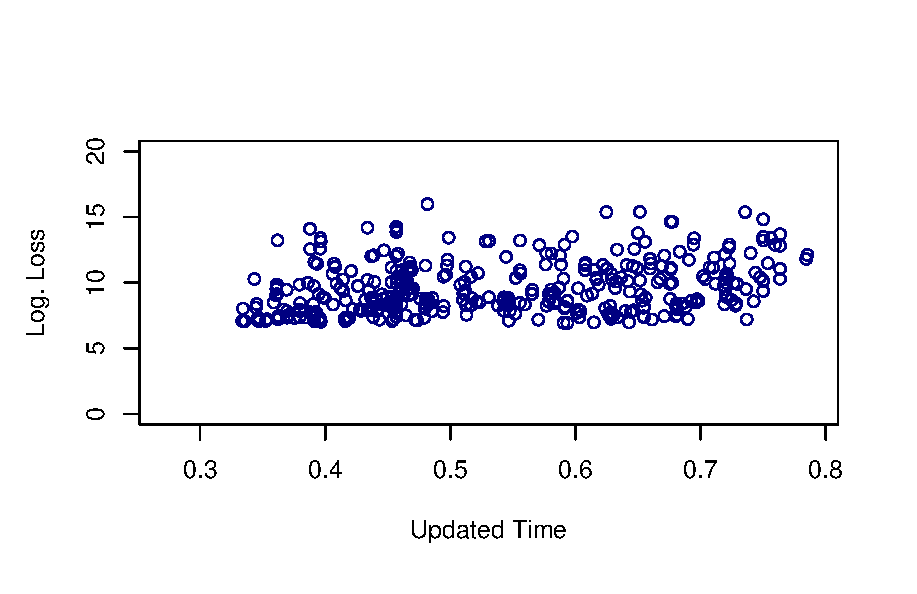
\includegraphics[width=7.5cm]{IntraDayUpdatedTime.eps}
         &
         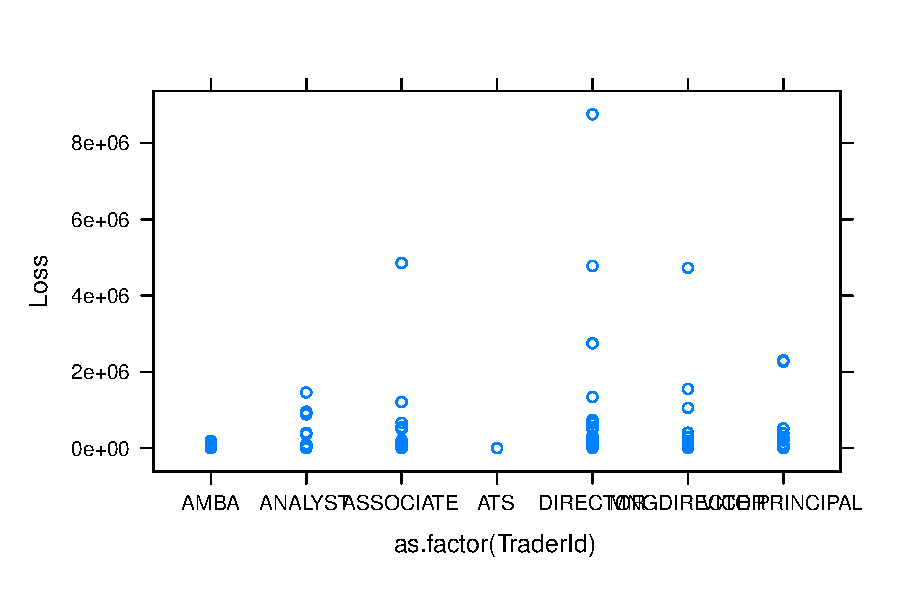
\includegraphics[width=7cm]{TrendTraderId.eps}
         \end{tabular}
    \end{frame}
\subcaption{Scatterplots}
   \label{Intra_Day_Trends} 
\end{subfigure}

\begin{subfigure}[b]{0.55\textwidth}
   \begin{frame}
      \centering
       \begin{tabular}{cc}
        \textbf{Loss per month} & \textbf{Trading frequency} \\
        \includegraphics[width=7.5cm]{UpdatedDayFreq.eps}
         &
         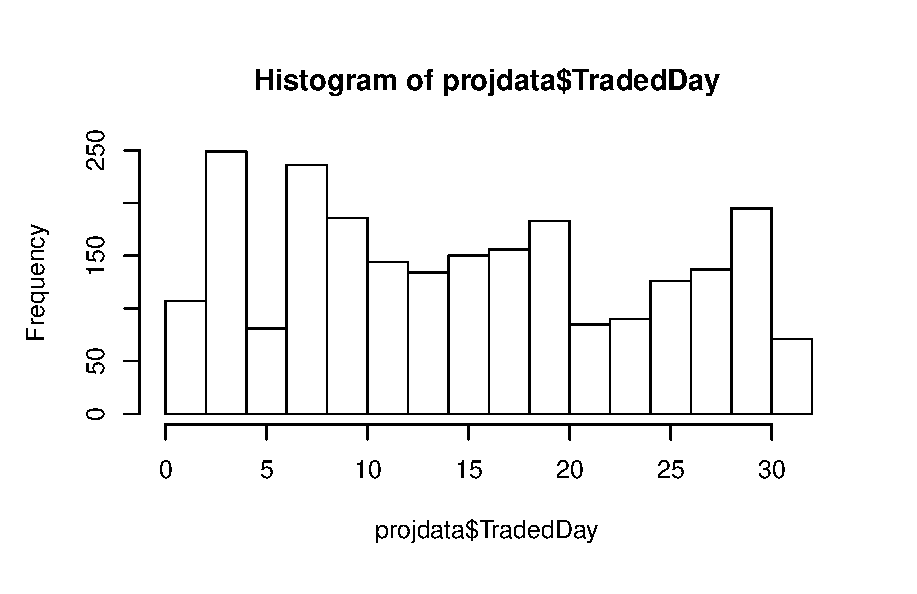
\includegraphics[width=7cm]{TradedDayFreq.eps}
         \end{tabular}
    \end{frame}
\subcaption{Histograms}
   \label{Hist_Loss_Freq}
\end{subfigure}
\caption[Numerical grid display]{(a) Scatterplots of intra-day trend analysis for logs of severities of operational events and trends incident activity for identifying the role of the trader originating the incidents. (b) As for (a) but in the form of histograms showing the frequency distrbution of the number daily operational indicents and the number of trades over a monthly period.} 
\end{figure}

\subsection{Characteristics of exposure}

The exposure of risk of type \(i\), \(d_i\) shows the daily duration,
from when the trade was booked to the moment the operational risk event
was observed and ended. This measure is defined this way when
specifically applied to projecting the number of loss events
(frequencies) and can be plotted as follows depicted in graphs depicted
in Figure \ref{Exploration_analysis_exposure}.\medskip

\begin{verbatim}
## 
## Attaching package: 'reshape'
\end{verbatim}

\begin{verbatim}
## The following object is masked from 'package:dplyr':
## 
##     rename
\end{verbatim}

\begin{figure}
\begin{frame}
      \centering
       \begin{tabular}{ccc}
        \textbf{Distribution} & \textbf{Density} & \textbf{Digital Analysis} \\
        \includegraphics[width=5cm]{Exposure_cdf.eps}
         &
         \includegraphics[width=5cm]{Dist_exposure.eps}
         &
         \includegraphics[width=5cm]{Benford.eps}
         \end{tabular}
    \end{frame}
        \captionof{figure}{A simple comparison of the Sigmoidal like features of the fat-tailed, right skewed distribution for exposure, and first-digit frequency distribution from the exposure data with the expected distribution according to Benford's Law}
    \label{Exploration_analysis_exposure}
\end{figure}

The variable follows a logistic trend on \([0,1]\), implying an FIs
operational risk portfolio rises like a sigmoid function throughout the
period of observation, typically starting from \(0\), which then
observes a plateau in growth. The average exposure is 389.99 or about 1
year.\medskip

Grid plots \ref{Exploration_analysis_exposure} portray the logistic
function, together with a simple comparison of first-digit frequency
distribution analysis, according to Benford's Law, with exposure data
distribution. The close fitting nature implies the data are uniformly
distributed across several orders of magnitude, especially within the 1
year period.\medskip

\subsection{Characteristics of the covariates}

The characteristics of the operational risk portfolio are given by the
following covariates: \emph{UpdatedDay}, \emph{UpdatedTime} - the day of
the month and time of day the OpRisk incident occurs respectively;
\emph{TradedDay}, \emph{TradedTime} - the day in the month and time of
day the deal was originated respectively; The \emph{LossIndicator} as
indicated before is a binary variable consisting of two values: A \(0\),
which indicates pending or near misses, and \(1\), if the incident
results in a realised loss, meaning that there is significant p\&L
impact due to the OpRisk incident.\medskip

the \emph{Desk} is the location in the portfolio tree the incident
originated, it is a factor variable conisting of 10 categories;
\emph{CapturedBy}, the designated analyst who actions the incident, a
factor variable consisting of 5 categories; \emph{TraderId}, the trader
who originates the deal, a factor variable with 7 categories;
\emph{TradeStatus}, the live status of the deal, a factor variable with
4 categories; \emph{Instrument}, the type of deal, a factor variable
with 23 categories; \emph{Reason}, a description of the cause of the
OpRisk incident, a factor variable with 19 levels;
\emph{EventTypeCategoryLevel}, 7 OpRisk event types as per
@risk2001supporting, a factor variable with 5 categories;
\emph{BusinessLineLevel}, 8 OpRisk business lines as per
@risk2001supporting, a factor variable with 8 categories.\medskip

\singlespacing

\begin{verbatim}
## Note: zip::zip() is deprecated, please use zip::zipr() instead
\end{verbatim}

\doublespacing

The continuous numerical variable \emph{Loss}, shows the financial
impact (severity) of the OpRisk incident in Rands. For the most part
(i.e.~96.1\% of the time) OpRisk incidents result in pending losses
and/or near misses, most realised losses (2.3\%) lie within the
{[}\textbf{R$200,00$}, \textbf{R$300,000$}{]} range. In the current
portfolio there are also five p\&L impacts higher than
\textbf{R$2.5$ million}.\medskip

\subsection{Characteristics of daily operational activity}

The distribution of daily losses and/or pending/near misses by
operational activities are represented in
\ref{Exploratory_Time_Day_Frequency3plot}. Figure
\ref{Exploratory_UpdateTime_Frequency3plot} shows that most operational
events occur in times leading up to midday (i.e.~10:50AM to 11:50AM),
the observed median is 11:39AM, and of these potential loss events, most
realised losses occur closest to mid-day. The frequencies of the loss
incidents in the analysed portfolio sharply decreases during the
following period, i.e.~from 12:10PM to 13:10PM, during which the least
realised losses occur.\medskip

Figure \ref{Exploratory_UpdateDay_Frequency3plot} shows that operational
activity increases in intensity in the days leading up to the middle of
the month, i.e.~\(10^{th}\) - \(15^{th}\); the observed mean is
\(14.49\) days, and of these potential loss events, realised losses
especially impact on the portfolio during these days.

\singlespacing

\doublespacing

\begin{figure}
\centering
\begin{subfigure}[b]{0.55\textwidth}
   \includegraphics[width=1.5\linewidth]{Exploratory_UpdateTime_Frequency3plot.eps}
   \subcaption{Frequency distributions of operational incidents by the time in the day}
   \label{Exploratory_UpdateTime_Frequency3plot} 
\end{subfigure}

\begin{subfigure}[b]{0.55\textwidth}
   \includegraphics[width=1.5\linewidth]{Exploratory_UpdateDay_Frequency3plot.eps}
   \subcaption{Frequency distributions of operational incidents by the day in the month}
   \label{Exploratory_UpdateDay_Frequency3plot}
\end{subfigure}

\caption[Two numerical solutions: Histograms showing the distribution of UpdatedTime \& UpdatedDay by LossIndicator.]{The frequency distributions of All the losses, the realised losses, and pending/near misses of operational incidents by the day in the month when the indidents' occurred}
\label{Exploratory_Time_Day_Frequency3plot}
\end{figure}

Similarly, the influence of trading desk's on the frequency of
operational events can be analysed on the basis of the portfolio's
bidimensional distribution by variables \emph{Desk} and
\emph{LossIndicator}, which shows the proportions realised losses vs
pending and/or near misses for each particular desk. The bidimensional
distribution of \emph{Desk} and \emph{LossIndicator} is presented in a
contingency table, Table \ref{tab_Desk_Prop}, in which it's considered
useful to calculate proportions for each desk category.

\begin{figure}
\centering
\includegraphics[width=15cm,height=5cm]{Density_UpdateDay_TradedDay.eps}
\caption[Density plots showing a comparison of realised vs pending losses and/near misses over a month for the day in the month the OpRisk incident was updated to the day in the month trades were traded/booked]{Density plots showing a comparison of realised vs pending losses and/near misses over a month for the day in the month the OpRisk incident was updated to the day in the month trades were traded/booked}
\label{Desk_Proportions}
\end{figure}

\singlespacing

\doublespacing

\begin{table}[ht]
\centering
\caption{Occurence of realised losses: proportions on desk categories}
\begin{tabular}{lccr}
\toprule
  & \multicolumn{3}{c}{No. of transactions} \\
Desk   & no Loss   & Loss & Total\\ 
\midrule
  Africa            &  49 & 10 &  59 \\
  Bonds/Repos       & 113 & 31 & 144 \\
  Commodities       & 282 & 45 & 327 \\
  Derivatives       & 205 & 24 & 229 \\
  Equity            & 269 & 66 & 335 \\
  Management/Other  &  41 &  2 &  43 \\
  Money Market      & 169 & 52 & 221 \\
  Prime Services    & 220 & 62 & 282 \\
  Rates             & 336 & 53 & 389 \\
  Structured Notes  & 275 & 26 & 301 \\
 \bottomrule
\end{tabular}\label{tab_Desk_Prop}
\end{table}

Thus, as illustratred in figure \ref{Desk_Proportions}, from 23,5\%; the
highest proportion of realised losses per desk is the Money Market (MM)
desk, the figures are decreasing, followed by Prime Services (22\%);
Bonds/Repos (21,5\%); Equity (19,7\%); Africa (16,9\%); Commodities
(13,8\%); Rates (13,6\%); Derivatives (10,5\%); Structured Notes (SND)
(8.6\%), to the least proportion in the Management/Other, a category
where only 4,7\% of operations activities were realised as losses.

\singlespacing

\begin{verbatim}
## Joining, by = "Desk"
\end{verbatim}

\doublespacing

\begin{figure}
\centering
\includegraphics[width=15cm,height=5cm]{Exploratory_Desk_Proportions.eps}
\caption[Desk category by realised losses]{Histograms showing the proportions of realised losses vs all losses including pending and/or near misses by desk category}
\label{Desk_Proportions}
\end{figure}

This behaviour can be extended beyond the trading desk, as represented
in Figure \ref{Mosaic_Instr_Trd_Tec}, a mosaic plot grid presenting the
structure of the OpRisk portfolio by Instrument, TraderId, CapturedBy
\footnote{i.e. the type of financial instrument, the trader who originated the incident on the deal, and the role of the technical support personnel who is involved in the query resolution.}
and the operational losses.

\singlespacing

\doublespacing

\begin{figure}
\begin{frame}
      \centering
       \begin{tabular}{cc}
        \textbf{Type of instrument traded} & \textbf{Role identification} \\
        \includegraphics[width=7.5cm,height=15cm]{Single_Instr.eps}
         &
         \includegraphics[width=7.5cm,height=15cm]{Stacked_TrId_TechSup.eps}
         \end{tabular}
    \end{frame}
    \caption{Mosaic grid plots for the bidimensional distribution by traded instrument, the trader originating the operational event, and by the technical support personnel involved in query resolution, against the dummy variable showing if a realised loss was reported.}
    \label{Mosaic_Instr_Trd_Tec}
\end{figure}

One can notice that the width of the bars corresponding to the different
categories, i.e.~Instrument, TraderId, CapturedBy, is given by their
proportion in the sample. In particular, for the category `at least one
realised loss', in the top right mosaic of Figure
\ref{Mosaic_Instr_Trd_Tec} portrays a increase in ``riskiness'' trending
up from Associate to AMBA, Analyst, Vice Principal, Managing Director,
Director, up to the risky ATS category, which are automated trading
system generated trades.\medskip

Figure \ref{Mosaic_Instr_Trd_Tec} bottom right mosaic plot for technical
support personnel for the category `at least one realised loss',
portrays a downward trend, slowing in riskiness from Unauthorised User
downward to Tech Support, Mid Office, Prod Controller down to the least
risky Prod Accountant. This intepretation makes sense given unauthorised
users are more likely to make impactful operational errors, technical
support personnel would also be accountable for large impacts albiet for
contrasting reasons, they are mandated to perform these deal adjustments
which have unavoidable impacts associated with them, whereas the former
group are unauthorised to perform adjustments therefore may lack the
skill, or be criminally minded insiders acting on their own or in unison
to enable their underhanded practices and intentions without raising any
suspicion.\medskip   

\begin{table}[!htbp] \centering 
  \caption{Summary statistics for all losses as per Instrument type} 
  \label{Stargazer} 
\begin{tabular}{@{\extracolsep{5pt}}lccccccc} 
\\[-1.8ex]\hline 
\hline \\[-1.8ex] 
Statistic & \multicolumn{1}{c}{N} & \multicolumn{1}{c}{Mean} & \multicolumn{1}{c}{St. Dev.} & \multicolumn{1}{c}{Min} & \multicolumn{1}{c}{Pctl(25)} & \multicolumn{1}{c}{Pctl(75)} & \multicolumn{1}{c}{Max} \\ 
\hline \\[-1.8ex] 
Mean & 23 & 34,603 & 46,007 & 306 & 7,697 & 44,157 & 192,513 \\ 
\hline \\[-1.8ex] 
\end{tabular} 
\end{table}

In another mosaic plot, Figure \ref{Mosaic_Contingency}, the
bidimensional distribution of transactions by trader and realised vs
pending losses, conditional on the trade status is presented and
analysed. Here, and in the contingency table, Table
\ref{tab:Mosaic_Contingency}, we can clearly see the following trends:
In BO-BO confirmed status - an increase in realised losses from the
leftmost TraderID (i.e.~AMBA) to right, and the opposite for
transactions performed in BO Confirmed status (both with two
exceptions). In particular, the biggest number of realised losses in
both BO and BO-BO Confirmed statuses occur due to automated trading
systems (ATS) who also give rise to the exceptions mentioned.\medskip

\singlespacing

\begin{verbatim}
## Loading required package: grid
\end{verbatim}

\singlespacing
\begin{figure}
\centering
\textbf{Mosasic plot for trader identification and loss indicator, by trade status}
\includegraphics[width=\linewidth,height=0.75\linewidth]{Mosaic_Contingency.eps}
\caption[Portfolio structure by trader, trade status and number of realised losses]{A mosaic plot representing the structure of the operational risk portfolio by trader identification (TraderId), the status ofthe trade (TradeStatus) and the number of realised losses vs pending or near misses}
\label{Mosaic_Contingency}
\end{figure}
\doublespacing

Table \ref{tab:Crosstab_covariate} presents the most frequent category
in the operational risk dataset for each possible covariate.

\begin{table}[htbp]
        \centering
        \textbf{Crosstab of trader identification and loss indicator, by trade status}
\singlespacing        
        \small
        \setlength\tabcolsep{2pt}
            \begin{tabular}{|p{2cm}|p{2cm}|l|l|l|l|l|l|p{2cm}|p{2cm}|} \hline
            & & \multicolumn{7}{|c|}{Trader Identification} \\ \hline
            TradeStatus & Loss Indicator & Amba & Analyst & Associate & ATS & Director & Mng Director & Vice Principal \\\hline
            \multirow{2}{*}{BO-BO Confirmed} & 0 & 24 & 136 & 320 & 0 & 282 & 52 & 49 \\ \cline{2-9}
                                   & 1 & 2  &  15 & 43 & 0 & 50 & 18 & 16 \\\cline{2-9}
            \multirow{2}{*}{BO Confirmed} & 0 & 17  & 299 & 153 & 13 & 257 & 102 & 153 \\ \cline{2-9}
                                   & 1 &  3 &  71 & 12 & 8 &  62 & 23 & 30 \\ \cline{2-9}
            \multirow{2}{*}{Terminated}       & 0 & 83 & 9 & 1 & 0 & 0 & 2 & 1 \\ \cline{2-9}
                                  & 1 & 17 & 1 & 0 & 0 & 0 & 0 & 0 \\ \cline{2-9}
            \multirow{2}{*}{Terminated/Void}  & 0 & 2 & 0 & 0 & 0 & 2 & 1 & 1 \\ \cline{2-9}
                                   & 1 & 0 & 0 & 0 & 0 & 0 & 0 & 0 \\ \hline
            \end{tabular}
            \caption{A contingency table showing the bidimensional distribution of transactions by trader identification vs realised and/or pending losses, conditional on the trade status}
            \label{tab:Crosstab_covariate}
\end{table}
\doublespacing

\begin{table}[htbp]
        \centering
        \textbf{Modal classes for the categorical variables} 
\singlespacing        
        \small
        \setlength\tabcolsep{2pt}
            \begin{tabular}{|l|l|p{4cm}|} \hline
            Variable & Modal class or category & Name of modal class \\\hline
            Desk & Rates & DeskRates \\ \cline{1-3}
            CapturedBy & TECHSUPPORT & CapturedBy\_TECHSUPPORT \\ \cline{1-3}
            TradeStatus & BO confirmed & TradeStatus\_BO confirmed \\ \cline{1-3}
            TraderId & DIRECTOR & TraderId\_DIRECTOR \\ \cline{1-3}
            Instrument & Swap & Instrument\_Swap \\ \cline{1-3}
            Reason & Trade enrichment for system flow  & Reason\_Trade enrichment for system flow \\ \cline{1-3}
            EventTypeCategoryLevel & EL7 & EventTypeCategoryLevel\_EL7 \\ \cline{1-3}
            BusinessLineLevel & BL2 & BusinessLineLevel\_BL2 \\ \cline{1-3} 
            \end{tabular}
            \caption{A contingency table showing the bidimensional distribution of transactions by trader identification vs realised and/or pending losses, conditional on the trade status}
            \label{tab:Mosaic_Contingency}
\end{table}
\doublespacing

\section{The estimation of some poisson regression generalised linear models (GLM's)}
\label{sec:The estimation of some poisson regression generalised linear models (GLM's)}

Section \ref{sec:Generalised Linear Models} introduced a GLM for the
start of the expected number of operational events in the early stages.
We aim to estimate the mean OpRisk frequency through a poisson
classification model given by equation \ref{eqn:Poisson} using the glm
function. The mean daily loss frequency in the risk correction
statistics is estimated through the poisson regression model. Let us
consider a model where the \emph{LossIndicator} is the target variable:
The following fits the model (the log link is canonical for the poisson
distribution, and hence the R default) and checks it.\medskip

\singlespacing

\doublespacing

In calling the GLM we specify the target variable \emph{LossIndicator};
the explanatory variables are composed of numeric, continuous and
categorical variables. Where the variable in the argument of a GLM is
categorical , one chose to specify the modal class as the reference
level. A user defined function ``getmode'' has been created; it selects
the modal observation in each factor, and the dataset is reordered using
the \emph{relevel} function in RStudio.

\singlespacing

\doublespacing

Other GLM arguments are: The afore-mentioned link function
poisson(link=``log''); a data frame containing the OpRisk dataset,
data=crs\$training; and the r offset=log(exposure), i.e.~the variable
representing a component known apriori, coefficient= \(1\), introduced
in the linear predictor {[}@covrig2015using{]}.\medskip

Firstly, consider a GLM in which is introduced two explanatory
variables, one numerical variable, \emph{UpdatedTime}, and another
categorical variable \emph{Desk}. This will be our global model. We will
use \emph{LossesIndicator} as the target variable, while these two
unique variables will be explanatory variables:

\singlespacing

\begin{Shaded}
\begin{Highlighting}[]
\NormalTok{freqfit1 <-}\StringTok{ }\KeywordTok{glm}\NormalTok{(LossesIndicator }\OperatorTok{~}\StringTok{ }\NormalTok{TradedDay }\OperatorTok{+}\StringTok{ }\NormalTok{Desk, }\DataTypeTok{data=}\NormalTok{crs}\OperatorTok{$}\NormalTok{training, }
               \DataTypeTok{family=}\KeywordTok{poisson}\NormalTok{(}\DataTypeTok{link =} \StringTok{'log'}\NormalTok{), }\DataTypeTok{offset =} \KeywordTok{log}\NormalTok{(Exposure))}
\end{Highlighting}
\end{Shaded}

\doublespacing

The output result of the estimation is presented below, where variables
who were found to be significant predictors are indicated. The
coefficients of the categorical variable \emph{Desk} are reordered and
weighted against the modal class: \emph{DeskRates}. Interestingly the
modal class does not show up in the results section (as the coefficient
of the modal class = \(0\)), given that the remaining classes are
weighted against it.

\singlespacing

\begin{verbatim}
## 
## Call:
## glm(formula = LossesIndicator ~ TradedDay + Desk, family = poisson(link = "log"), 
##     data = crs$training, offset = log(Exposure))
## 
## Deviance Residuals: 
##     Min       1Q   Median       3Q      Max  
## -2.9946  -0.5576  -0.2284  -0.0517   4.3648  
## 
## Coefficients:
##                        Estimate Std. Error z value             Pr(>|z|)
## (Intercept)           -8.022977   0.192289 -41.724 < 0.0000000000000002
## TradedDay             -0.013556   0.006385  -2.123             0.033759
## DeskAfrica             1.402399   0.388993   3.605             0.000312
## DeskBonds/Repos        1.981497   0.251700   7.872  0.00000000000000348
## DeskCommodities        0.765467   0.240063   3.189             0.001430
## DeskDerivatives       -0.072921   0.272344  -0.268             0.788889
## DeskEquity             1.326918   0.220486   6.018  0.00000000176424133
## DeskManagement/Other -14.044212 289.296857  -0.049             0.961281
## DeskMM                 0.255313   0.238297   1.071             0.283985
## DeskPrime Services     2.208663   0.217438  10.158 < 0.0000000000000002
## DeskSND               -0.714792   0.272087  -2.627             0.008612
##                         
## (Intercept)          ***
## TradedDay            *  
## DeskAfrica           ***
## DeskBonds/Repos      ***
## DeskCommodities      ** 
## DeskDerivatives         
## DeskEquity           ***
## DeskManagement/Other    
## DeskMM                  
## DeskPrime Services   ***
## DeskSND              ** 
## ---
## Signif. codes:  0 '***' 0.001 '**' 0.01 '*' 0.05 '.' 0.1 ' ' 1
## 
## (Dispersion parameter for poisson family taken to be 1)
## 
##     Null deviance: 2089.9  on 1746  degrees of freedom
## Residual deviance: 1835.4  on 1736  degrees of freedom
## AIC: 2411.4
## 
## Number of Fisher Scoring iterations: 15
\end{verbatim}

\doublespacing

Using this bivariate model, the estimated quarterly OpRisk
(LossIndicators) frequency of realised losses for each \emph{Desk}
category (excluding the insignificant ones) are:

\begin{list}{*}{}
\item $0,0012 = e^{-7.99905}\cdot e^{-0.01427}\cdot e^{1.28441}$, for the combination of the \textbf{UpdateTime} and \textbf{DeskAfrica} category, which implies that frequency of realised losses for this combination of preditor variables is $3.613 (=\cdot e^{1.28441})$ fold (times) higher than the realised loss frequency of OpRisk causes in the reference desk category, viz. the \textbf{Rates} desk. 
\item $0,0021 = e^{-7.99905}\cdot e^{-0.01427}\cdot e^{1.86747}$, for the combination of the \textbf{UpdateTime} and \textbf{DeskBonds/Repos} category, which implies that frequency of realised losses for this combination of preditor variables is $6,472(=\cdot e^{1.86747})$ fold higher than causes in the reference desk category.
\item $0,0007 = e^{-7.99905}\cdot e^{-0.01427}\cdot e^{0.72735}$, for the combination, which implies that frequency of realised losses for this combination of preditor variables is $2,070(=\cdot e^{0.72735})$ fold higher than the causes in the reference desk category.
\item $0,0012 = e^{-7.99905}\cdot e^{-0.01427}\cdot e^{1.31836}$, for the combination, which implies that frequency of realised losses for this combination of preditor variables is $3,737(=\cdot e^{1.31836})$ fold higher than the causes in the reference desk category.
\item $0,001373903 = e^{-7.99905}\cdot e^{-0.01427}\cdot e^{2.15462}$, for the combination with \textbf{DeskPrime Services},an increase of $8,625(=\cdot e^{2.15472})$ fold times higher w.r.t the baseline (the \textbf{Rates} desk)
\item about $0.00000025 = e^{-7.99905}\cdot e^{-0.01427}\cdot e^{-0.71920}$ of the last desk category \textbf{DeskSND}, which means a decrease of about 50% of the frequency of losses in the \textbf{DeskRates} category.
\end{list}

The predicted mean frequency of realised losses for OpRisk incident
\(i\), for the model \textbf{freqfit1}, is given by:

\singlespacing

\begin{eqnarray}
\mu_{i}& = &\mbox{exposure}_i\cdot e^{-7.99905\cdot \mbox{Intercept}_i}\cdot e^{-0.01427\cdot \mbox{UpdatedTime}_i}\cdot e^{1.28441\cdot \mbox{DeskAfrica}_i}\nonumber\\
&\cdot&e^{1.86747\cdot \mbox{DeskBonds/Repos}_i}\cdot e^{0.72735\cdot \mbox{DeskCommodities}_i}\cdot e^{1.31836\cdot \mbox{DeskEquity}_i}\nonumber\\
&\cdot& e^{2.15462\cdot \mbox{DeskPrime Services}_i}\cdot e^{-0.71920\cdot \mbox{DeskSND}_i}
\end{eqnarray} \doublespacing

We now fit a more comprehensive model where we introduce more variables,
in which show realised losses for quarterly OpRisk incidents for an all
inclusive case. We will use ``LossesIndicator'' as the dependent
variable, while the other variables will be predictor variables.

\singlespacing

\begin{Shaded}
\begin{Highlighting}[]
\CommentTok{### Let us fit a GLM to our data. This will be our global model. use "LossesIndicator"}
\CommentTok{#as the dependent variable, while the other variables will be predictor variables.}
\NormalTok{freqfit <-}\StringTok{ }\KeywordTok{glm}\NormalTok{(LossesIndicator }\OperatorTok{~}\StringTok{ }\NormalTok{UpdatedDay }\OperatorTok{+}\StringTok{ }\NormalTok{UpdatedTime }\OperatorTok{+}
\StringTok{                 }\NormalTok{TradedDay }\OperatorTok{+}\StringTok{ }\NormalTok{TradedTime }\OperatorTok{+}\StringTok{ }\NormalTok{Desk }\OperatorTok{+}\StringTok{ }\NormalTok{CapturedBy }\OperatorTok{+}
\StringTok{                 }\NormalTok{TradeStatus }\OperatorTok{+}\StringTok{ }\NormalTok{TraderId }\OperatorTok{+}\StringTok{ }\NormalTok{Instrument }\OperatorTok{+}\StringTok{ }\NormalTok{Reason}
               \OperatorTok{+}\StringTok{ }\NormalTok{EventTypeCategoryLevel1 }\OperatorTok{+}\StringTok{ }\NormalTok{BusinessLineLevel1,}
\DataTypeTok{data=}\NormalTok{crs}\OperatorTok{$}\NormalTok{training, }\DataTypeTok{family=}\KeywordTok{poisson}\NormalTok{(}\DataTypeTok{link =} \StringTok{'log'}\NormalTok{), }\DataTypeTok{offset =} \KeywordTok{log}\NormalTok{(Exposure))}
\end{Highlighting}
\end{Shaded}

\doublespacing

Which yields output (in summarised form):

\singlespacing
\begin{verbatim}
Call:
glm(formula = LossesIndicator ~ UpdatedDay + UpdatedTime + TradedDay + 
    TradedTime + Desk + CapturedBy + TradeStatus + TraderId + 
    Instrument + Reason + EventTypeCategoryLevel1 + BusinessLineLevel1, 
    family = poisson(link = "log"), data = crs$training, offset = log(Exposure))

Deviance Residuals: 
    Min       1Q   Median       3Q      Max  
-3.7328  -0.3616  -0.1012  -0.0139   4.1107  

Coefficients:
                        Estimate  Std. Error z value  (Intercept)         
(Intercept)             -8.601892    0.738478 -11.648   < 0.0000000000000002 ***
UpdatedDay              -0.014075    0.010414  -1.352    0.17651
UpdatedTime              0.105966    0.708733   0.150    0.88115 
TradedDay               -0.015601    0.008275  -1.885    0.05939 .
TradedTime               0.252615    0.782853   0.323    0.74693
DeskAfrica               2.388334    0.575306   4.151    0.000033042768080 ***
DeskBonds/Repos          2.975192    0.442633   6.722    0.000000000017977 ***
DeskCommodities          1.142290    0.474629   2.407    0.01610 *
DeskDerivatives          0.952777    0.491440   1.939    0.05253 . 
DeskEquity               1.745408    0.427535   4.082    0.000044556065633 ***
DeskManagement/Other    -15.024612  620.154848  -0.024    0.98067
DeskMM                   1.692119    0.583820   2.898    0.00375 ** 
DeskPrime Services       0.310749    1.303433   0.238    0.81156 
DeskSND                  1.100596    0.726644   1.515    0.12987                                 
     .                      .           .         .         .
     .                      .           .         .         .
     .                      .           .         .         .
BusinessLineLevel1BL1    1.698196    0.729494   2.328   0.01992 *
BusinessLineLevel1BL3   -0.177178    0.652274  -0.272   0.78590
BusinessLineLevel1BL4   -1.547668    0.494473  -3.130   0.00175 **
BusinessLineLevel1BL5   -1.146241    0.501862  -2.284   0.02237 *
BusinessLineLevel1BL6    1.733747    1.354626   1.280   0.20059
BusinessLineLevel1BL7    1.593485    2.598998   0.613   0.53980
BusinessLineLevel1BL9    1.871917 1328.440227   0.001   0.99888 
---
Signif. codes:  0 ‘***’ 0.001 ‘**’ 0.01 ‘*’ 0.05 ‘.’ 0.1 ‘ ’ 1

(Dispersion parameter for poisson family taken to be 1)

    Null deviance: 1943.5  on 1630  degrees of freedom
Residual deviance: 1239.6  on 1553  degrees of freedom
AIC: 1907.6

Number of Fisher Scoring iterations: 16

\end{verbatim}
\doublespacing

\singlespacing

\doublespacing

\subsubsection{Model selection and multimodel inference}

The selection of the best-fit model from the list of possible
combinations of predictor variables traditionally follows of a process
removing/adding each variable progressively after each estimation, and
propagating backward/forward, comparing goodnes of fit tests at each
stage. For example, if we compare the values of the Aikaike information
criteria (AIC) for the bivariate model \textbf{freqfit1} and the
multivariate model \textbf{freqfit}, by AICs; we see that for the first
(bivariate) model the AIC value is \(2253.4\) and \(1907.6\) for the
second (multivariate) model, which suggests that the second model,
\textbf{freqfit}, the model in which we considered an all inclusive list
of \(13\) predictor variables is a better fit since there is a marked
reduction/improvement in AIC magnitudes compared to the first value,
hence \textbf{freqfit} is prefered over the bivariate (first) model.
\medskip

similarly, an estimation of the models by a comparison which enables the
choice the most appropriate or ``best'' fit model, first through finding
out its significance, viz.~if the residual deviance and the
corresponding number of degrees of freedom doesn't have a value
significantly bigger than \(1\): In the multivariate model freqfit
\(\frac{1239.6}{1553} = 0.8\), and then retaining the model with the
smaller AIC value.\medskip 

@Burnham2002 introduction of an information-theoretic approach permits a
data-based selection for the ``best-fit'' model in the analysis of the
OpRisk dataset \emph{OpRiskDataSet\_exposure.csv}, and a ranking and
weighting of what remains. This approach allows traditional (formal)
statistical inference to be based on the selected ``best-fit'' model,
which is now based on more than one model (multimodel inference). As a
requirment the r package to load is the ``\textbf{MuMIn}'' Rstudio
package. \medskip

\singlespacing

\begin{verbatim}
## Loading required package: MuMIn
\end{verbatim}

\begin{verbatim}
## 
## Attaching package: 'MuMIn'
\end{verbatim}

\begin{verbatim}
## The following object is masked from 'package:rattle':
## 
##     importance
\end{verbatim}

\doublespacing

Then, we use ``dredge'' function to generate models using combinations
of the terms in the global model. The function will also calculate AICc
values and rank models according to it. Note that AICc is AIC corrected
for finite sample sizes. The process of analyzing data where the
experimentalist has few or no a priori information, thus ``all possible
models'' are considered by subjectively ad iteratively searching the
data for patterns and ``significance'', is often called ``data mining'',
``data snooping'' or the term ``data dredging''.

\singlespacing

\begin{verbatim}
## Fixed term is "(Intercept)"
\end{verbatim}

\doublespacing

The function ``MuMLn::dredge'' returns a list of \(4097\) models, which
is every combination of predictor variable in the global model freqfit.
Model number 894 is the best-fit: All predictor variables included in
this model have a positive effect on the target variable except for the
preditor TrddD (\textbf{TradedDay}) which has a negative effect on the
likelihood of a realised loss (target variable \emph{LossIndicator})
i.e., the later in the month of the transaction, the less likely a loss
is realised. Additionally, from the delta (=delta AIC) one cannot
distinguish between models 894, 382, 1918 and 1406 since (using the
common rule of thumb) they have AIC \textless{} 2.\medskip

Of the top seven models (listed below); 1918 \& 2942 each hold nine;
894, 1406 \& 1854 hold eight; 382 \& 830 hold seven; and lastly 318 hold
six predictor variables respectively. Where a variable doesn't have a
value associated with it does not mean no effect, but rather that it was
not included in the model. For example, model \(894\) returns a
combination of the eight variables \(1/2/3/4/5/6/7/8\), corresponding to
top most model in the following output predictor variables (abbreviated
in the header row) below:

\singlespacing
\begin{verbatim}
Global model call: glm(formula = LossesIndicator ~ UpdatedDay + UpdatedTime + TradedDay + 
    TradedTime + Desk + CapturedBy + TradeStatus + TraderId + 
    Instrument + Reason + EventTypeCategoryLevel1 + BusinessLineLevel1, 
    family = poisson(link = "log"), data = crs$training, 
    offset = log(Exposure))
---
Model selection table 
     (Intrc) BsLL1 Desk ETCL1 Instr Reasn   TrddD TrdrI TrdSt  UpdtD      UpdtT     df    logLik   AICc  delta weight
894   -8.566     + +     +     +     + -0.014630000 +     +                         71  -879.525 1907.6   0.00  0.082
382   -8.627     + +     +     +     + -0.014730000 +                               68  -882.870 1907.7   0.14  0.076
1918  -8.362     + +     +     +     + -0.015200000 +     + -0.012880000            72  -878.679 1908.1   0.50  0.064
1406  -8.447     + +     +     +     + -0.015290000 +       -0.011540000            69  -882.168 1908.5   0.92  0.052
830   -8.889     + +     +     +     +              +     +                         70  -881.128 1908.6   1.02  0.049
318   -8.942     + +     +     +     +              +                               67  -884.505 1908.8   1.23  0.044
1854  -8.705     + +     +     +     +              +     + -0.011920000            71  -880.413 1909.4   1.78  0.034
2942  -8.730     + +     +     +     + -0.014640000 +     +               0.3133000 72  -879.413 1909.6   1.97  0.031

\end{verbatim}
\doublespacing

Information from the AICc's values suggest, that of the top eight models
have similar support, and their Akaike weights are not high relative to
the \([0,1]\) weight range: This is characteristic of the endemic nature
of data dredging, as the literature suggests {[}@Burnham2002{]}, and
should generally be avoided to curb attendant inferential problems if a
single model is chosen, e.g the risk of finding spurious effects,
overfitting, etc. @Burnham2002 advises that model averaging is useful in
finding a confirmatory result as estimates of precision should include
model selection uncertainty. Even so, one can rule out many models on a
priori grounds.\medskip    

We now use ``get.models'' function to generate a list in which its
objects are the fitted models. We will also use the ``model.avg''
function to do a model averaging based on AICc. Note that
``subset=TRUE'' will make the function calculate the average model (or
mean model) using all models. However, we want to get only the models
that have delta AICc \textless{} 2; we threfore use
``subset=delta\textless{}2''

\singlespacing

\doublespacing

Now we have AICc values for our models and we have the average (mean)
model.\medskip

\singlespacing
\begin{verbatim}
Call:
model.avg(object = get.models(freqfits, subset = delta < 2))

Component model call: 
glm(formula = LossesIndicator ~ <8 unique rhs>, family = poisson(link = "log"),
data = crs$training, offset = log(Exposure))

Component models: 
                   df  logLik    AICc delta weight
1/2/3/4/5/6/7/8    71 -879.52 1907.61  0.00   0.19
1/2/3/4/5/6/7      68 -882.87 1907.75  0.14   0.18
1/2/3/4/5/6/7/8/9  72 -878.68 1908.11  0.50   0.15
1/2/3/4/5/6/7/9    69 -882.17 1908.53  0.92   0.12
1/2/3/4/5/7/8      70 -881.13 1908.63  1.02   0.11
1/2/3/4/5/7        67 -884.50 1908.84  1.23   0.10
1/2/3/4/5/7/8/9    71 -880.41 1909.38  1.78   0.08
1/2/3/4/5/6/7/8/10 72 -879.41 1909.57  1.97   0.07

Term codes: 
BusinessLineLevel1  Desk     EventTypeCategoryLevel1  Instrument  Reason 
1                   2        3                        4           5 
TradedDay           TraderId TradeStatus              UpdatedDay  UpdatedTime 
6                   7        8                        9           10 
\end{verbatim}
\doublespacing

Multimodel inference leads to more robust inferences, especially in the
point of view that the selection of the model used to estimate the mean
frequency must, at the same time, serve the ultimate root cause analysis
objective of OpRisk control, that decide calculating capital
requirement, in OpVaR measures, taking into account as many
characteristics of the trading OpRisk dataset as possible, as well
considering how the variables interact with each other.

\begin{verbatim}
## Warning in dpois(x, estimate, log = TRUE): non-integer x = 0.101165
\end{verbatim}

\begin{verbatim}
## Warning in dpois(x, estimate, log = TRUE): non-integer x = 0.005679
\end{verbatim}

\begin{verbatim}
## Warning in dpois(x, estimate, log = TRUE): non-integer x = 0.018796
\end{verbatim}

\begin{verbatim}
## Warning in dpois(x, estimate, log = TRUE): non-integer x = 0.003467
\end{verbatim}

\begin{verbatim}
## Warning in dpois(x, estimate, log = TRUE): non-integer x = 0.570012
\end{verbatim}

\begin{verbatim}
## Warning in dpois(x, estimate, log = TRUE): non-integer x = 0.014299
\end{verbatim}

\begin{verbatim}
## Warning in dpois(x, estimate, log = TRUE): non-integer x = 0.243765
\end{verbatim}

\begin{verbatim}
## Warning in dpois(x, estimate, log = TRUE): non-integer x = 0.000127
\end{verbatim}

\begin{verbatim}
## Warning in dpois(x, estimate, log = TRUE): non-integer x = 0.017156
\end{verbatim}

\begin{verbatim}
## Warning in dpois(x, estimate, log = TRUE): non-integer x = 0.064557
\end{verbatim}

\begin{verbatim}
## Warning in dpois(x, estimate, log = TRUE): non-integer x = 0.000039
\end{verbatim}

\begin{verbatim}
## Warning in dpois(x, estimate, log = TRUE): non-integer x = 0.011512
\end{verbatim}

\begin{verbatim}
## Warning in dpois(x, estimate, log = TRUE): non-integer x = 0.726716
\end{verbatim}

\begin{verbatim}
## Warning in dpois(x, estimate, log = TRUE): non-integer x = 0.065453
\end{verbatim}

\begin{verbatim}
## Warning in dpois(x, estimate, log = TRUE): non-integer x = 0.034140
\end{verbatim}

\begin{verbatim}
## Warning in dpois(x, estimate, log = TRUE): non-integer x = 0.012493
\end{verbatim}

\begin{verbatim}
## Warning in dpois(x, estimate, log = TRUE): non-integer x = 0.563256
\end{verbatim}

\begin{verbatim}
## Warning in dpois(x, estimate, log = TRUE): non-integer x = 1.885740
\end{verbatim}

\begin{verbatim}
## Warning in dpois(x, estimate, log = TRUE): non-integer x = 0.884763
\end{verbatim}

\begin{verbatim}
## Warning in dpois(x, estimate, log = TRUE): non-integer x = 0.887613
\end{verbatim}

\begin{verbatim}
## Warning in dpois(x, estimate, log = TRUE): non-integer x = 0.002972
\end{verbatim}

\begin{verbatim}
## Warning in dpois(x, estimate, log = TRUE): non-integer x = 0.056135
\end{verbatim}

\begin{verbatim}
## Warning in dpois(x, estimate, log = TRUE): non-integer x = 0.139852
\end{verbatim}

\begin{verbatim}
## Warning in dpois(x, estimate, log = TRUE): non-integer x = 0.000099
\end{verbatim}

\begin{verbatim}
## Warning in dpois(x, estimate, log = TRUE): non-integer x = 0.997224
\end{verbatim}

\begin{verbatim}
## Warning in dpois(x, estimate, log = TRUE): non-integer x = 0.001221
\end{verbatim}

\begin{verbatim}
## Warning in dpois(x, estimate, log = TRUE): non-integer x = 0.013999
\end{verbatim}

\begin{verbatim}
## Warning in dpois(x, estimate, log = TRUE): non-integer x = 0.024828
\end{verbatim}

\begin{verbatim}
## Warning in dpois(x, estimate, log = TRUE): non-integer x = 0.000141
\end{verbatim}

\begin{verbatim}
## Warning in dpois(x, estimate, log = TRUE): non-integer x = 0.000448
\end{verbatim}

\begin{verbatim}
## Warning in dpois(x, estimate, log = TRUE): non-integer x = 0.084837
\end{verbatim}

\begin{verbatim}
## Warning in dpois(x, estimate, log = TRUE): non-integer x = 0.731035
\end{verbatim}

\begin{verbatim}
## Warning in dpois(x, estimate, log = TRUE): non-integer x = 0.000242
\end{verbatim}

\begin{verbatim}
## Warning in dpois(x, estimate, log = TRUE): non-integer x = 0.000942
\end{verbatim}

\begin{verbatim}
## Warning in dpois(x, estimate, log = TRUE): non-integer x = 0.001759
\end{verbatim}

\begin{verbatim}
## Warning in dpois(x, estimate, log = TRUE): non-integer x = 0.005567
\end{verbatim}

\begin{verbatim}
## Warning in dpois(x, estimate, log = TRUE): non-integer x = 0.042701
\end{verbatim}

\begin{verbatim}
## Warning in dpois(x, estimate, log = TRUE): non-integer x = 0.014213
\end{verbatim}

\begin{verbatim}
## Warning in dpois(x, estimate, log = TRUE): non-integer x = 0.064194
\end{verbatim}

\begin{verbatim}
## Warning in dpois(x, estimate, log = TRUE): non-integer x = 0.005838
\end{verbatim}

\begin{verbatim}
## Warning in dpois(x, estimate, log = TRUE): non-integer x = 0.014855
\end{verbatim}

\begin{verbatim}
## Warning in dpois(x, estimate, log = TRUE): non-integer x = 0.005817
\end{verbatim}

\begin{verbatim}
## Warning in dpois(x, estimate, log = TRUE): non-integer x = 0.005187
\end{verbatim}

\begin{verbatim}
## Warning in dpois(x, estimate, log = TRUE): non-integer x = 0.004425
\end{verbatim}

\begin{verbatim}
## Warning in dpois(x, estimate, log = TRUE): non-integer x = 0.215420
\end{verbatim}

\begin{verbatim}
## Warning in dpois(x, estimate, log = TRUE): non-integer x = 0.007848
\end{verbatim}

\begin{verbatim}
## Warning in dpois(x, estimate, log = TRUE): non-integer x = 0.014215
\end{verbatim}

\begin{verbatim}
## Warning in dpois(x, estimate, log = TRUE): non-integer x = 0.148255
\end{verbatim}

\begin{verbatim}
## Warning in dpois(x, estimate, log = TRUE): non-integer x = 0.054704
\end{verbatim}

\begin{verbatim}
## Warning in dpois(x, estimate, log = TRUE): non-integer x = 0.004250
\end{verbatim}

\begin{verbatim}
## Warning in dpois(x, estimate, log = TRUE): non-integer x = 0.030525
\end{verbatim}

\begin{verbatim}
## Warning in dpois(x, estimate, log = TRUE): non-integer x = 0.000036
\end{verbatim}

\begin{verbatim}
## Warning in dpois(x, estimate, log = TRUE): non-integer x = 0.235909
\end{verbatim}

\begin{verbatim}
## Warning in dpois(x, estimate, log = TRUE): non-integer x = 0.019378
\end{verbatim}

\begin{verbatim}
## Warning in dpois(x, estimate, log = TRUE): non-integer x = 0.101165
\end{verbatim}

\begin{verbatim}
## Warning in dpois(x, estimate, log = TRUE): non-integer x = 0.011733
\end{verbatim}

\begin{verbatim}
## Warning in dpois(x, estimate, log = TRUE): non-integer x = 0.001046
\end{verbatim}

\begin{verbatim}
## Warning in dpois(x, estimate, log = TRUE): non-integer x = 0.027720
\end{verbatim}

\begin{verbatim}
## Warning in dpois(x, estimate, log = TRUE): non-integer x = 0.017722
\end{verbatim}

\begin{verbatim}
## Warning in dpois(x, estimate, log = TRUE): non-integer x = 0.006745
\end{verbatim}

\begin{verbatim}
## Warning in dpois(x, estimate, log = TRUE): non-integer x = 0.000886
\end{verbatim}

\begin{verbatim}
## Warning in dpois(x, estimate, log = TRUE): non-integer x = 0.286012
\end{verbatim}

\begin{verbatim}
## Warning in dpois(x, estimate, log = TRUE): non-integer x = 0.001604
\end{verbatim}

\begin{verbatim}
## Warning in dpois(x, estimate, log = TRUE): non-integer x = 0.036702
\end{verbatim}

\begin{verbatim}
## Warning in dpois(x, estimate, log = TRUE): non-integer x = 0.027349
\end{verbatim}

\begin{verbatim}
## Warning in dpois(x, estimate, log = TRUE): non-integer x = 0.460257
\end{verbatim}

\begin{verbatim}
## Warning in dpois(x, estimate, log = TRUE): non-integer x = 0.000120
\end{verbatim}

\begin{verbatim}
## Warning in dpois(x, estimate, log = TRUE): non-integer x = 0.014173
\end{verbatim}

\begin{verbatim}
## Warning in dpois(x, estimate, log = TRUE): non-integer x = 0.000757
\end{verbatim}

\begin{verbatim}
## Warning in dpois(x, estimate, log = TRUE): non-integer x = 0.217979
\end{verbatim}

\begin{verbatim}
## Warning in dpois(x, estimate, log = TRUE): non-integer x = 0.000450
\end{verbatim}

\begin{verbatim}
## Warning in dpois(x, estimate, log = TRUE): non-integer x = 0.014866
\end{verbatim}

\begin{verbatim}
## Warning in dpois(x, estimate, log = TRUE): non-integer x = 0.000023
\end{verbatim}

\begin{verbatim}
## Warning in dpois(x, estimate, log = TRUE): non-integer x = 0.000477
\end{verbatim}

\begin{verbatim}
## Warning in dpois(x, estimate, log = TRUE): non-integer x = 0.000732
\end{verbatim}

\begin{verbatim}
## Warning in dpois(x, estimate, log = TRUE): non-integer x = 0.000016
\end{verbatim}

\begin{verbatim}
## Warning in dpois(x, estimate, log = TRUE): non-integer x = 0.101165
\end{verbatim}

\begin{verbatim}
## Warning in dpois(x, estimate, log = TRUE): non-integer x = 0.000003
\end{verbatim}

\begin{verbatim}
## Warning in dpois(x, estimate, log = TRUE): non-integer x = 0.002678
\end{verbatim}

\begin{verbatim}
## Warning in dpois(x, estimate, log = TRUE): non-integer x = 0.000000
\end{verbatim}

\begin{verbatim}
## Warning in dpois(x, estimate, log = TRUE): non-integer x = 0.076544
\end{verbatim}

\begin{verbatim}
## Warning in dpois(x, estimate, log = TRUE): non-integer x = 0.000011
\end{verbatim}

\begin{verbatim}
## Warning in dpois(x, estimate, log = TRUE): non-integer x = 0.004391
\end{verbatim}

\begin{verbatim}
## Warning in dpois(x, estimate, log = TRUE): non-integer x = 0.000214
\end{verbatim}

\begin{verbatim}
## Warning in dpois(x, estimate, log = TRUE): non-integer x = 0.001059
\end{verbatim}

\begin{verbatim}
## Warning in dpois(x, estimate, log = TRUE): non-integer x = 0.005977
\end{verbatim}

\begin{verbatim}
## Warning in dpois(x, estimate, log = TRUE): non-integer x = 0.000245
\end{verbatim}

\begin{verbatim}
## Warning in dpois(x, estimate, log = TRUE): non-integer x = 0.000062
\end{verbatim}

\begin{verbatim}
## Warning in dpois(x, estimate, log = TRUE): non-integer x = 0.000077
\end{verbatim}

\begin{verbatim}
## Warning in dpois(x, estimate, log = TRUE): non-integer x = 0.259686
\end{verbatim}

\begin{verbatim}
## Warning in dpois(x, estimate, log = TRUE): non-integer x = 0.000527
\end{verbatim}

\begin{verbatim}
## Warning in dpois(x, estimate, log = TRUE): non-integer x = 0.002916
\end{verbatim}

\begin{verbatim}
## Warning in dpois(x, estimate, log = TRUE): non-integer x = 0.006460
\end{verbatim}

\begin{verbatim}
## Warning in dpois(x, estimate, log = TRUE): non-integer x = 0.704732
\end{verbatim}

\begin{verbatim}
## Warning in dpois(x, estimate, log = TRUE): non-integer x = 0.068169
\end{verbatim}

\begin{verbatim}
## Warning in dpois(x, estimate, log = TRUE): non-integer x = 0.004749
\end{verbatim}

\begin{verbatim}
## Warning in dpois(x, estimate, log = TRUE): non-integer x = 0.005150
\end{verbatim}

\begin{verbatim}
## Warning in dpois(x, estimate, log = TRUE): non-integer x = 0.230409
\end{verbatim}

\begin{verbatim}
## Warning in dpois(x, estimate, log = TRUE): non-integer x = 0.013752
\end{verbatim}

\begin{verbatim}
## Warning in dpois(x, estimate, log = TRUE): non-integer x = 0.225656
\end{verbatim}

\begin{verbatim}
## Warning in dpois(x, estimate, log = TRUE): non-integer x = 0.021781
\end{verbatim}

\begin{verbatim}
## Warning in dpois(x, estimate, log = TRUE): non-integer x = 0.045975
\end{verbatim}

\begin{verbatim}
## Warning in dpois(x, estimate, log = TRUE): non-integer x = 0.367394
\end{verbatim}

\begin{verbatim}
## Warning in dpois(x, estimate, log = TRUE): non-integer x = 0.001529
\end{verbatim}

\begin{verbatim}
## Warning in dpois(x, estimate, log = TRUE): non-integer x = 0.000268
\end{verbatim}

\begin{verbatim}
## Warning in dpois(x, estimate, log = TRUE): non-integer x = 0.080267
\end{verbatim}

\begin{verbatim}
## Warning in dpois(x, estimate, log = TRUE): non-integer x = 0.000944
\end{verbatim}

\begin{verbatim}
## Warning in dpois(x, estimate, log = TRUE): non-integer x = 0.063734
\end{verbatim}

\begin{verbatim}
## Warning in dpois(x, estimate, log = TRUE): non-integer x = 0.011793
\end{verbatim}

\begin{verbatim}
## Warning in dpois(x, estimate, log = TRUE): non-integer x = 0.587671
\end{verbatim}

\begin{verbatim}
## Warning in dpois(x, estimate, log = TRUE): non-integer x = 0.000047
\end{verbatim}

\begin{verbatim}
## Warning in dpois(x, estimate, log = TRUE): non-integer x = 0.449150
\end{verbatim}

\begin{verbatim}
## Warning in dpois(x, estimate, log = TRUE): non-integer x = 0.844180
\end{verbatim}

\begin{verbatim}
## Warning in dpois(x, estimate, log = TRUE): non-integer x = 0.199020
\end{verbatim}

\begin{verbatim}
## Warning in dpois(x, estimate, log = TRUE): non-integer x = 0.003719
\end{verbatim}

\begin{verbatim}
## Warning in dpois(x, estimate, log = TRUE): non-integer x = 0.002695
\end{verbatim}

\begin{verbatim}
## Warning in dpois(x, estimate, log = TRUE): non-integer x = 0.051364
\end{verbatim}

\begin{verbatim}
## Warning in dpois(x, estimate, log = TRUE): non-integer x = 0.098080
\end{verbatim}

\begin{verbatim}
## Warning in dpois(x, estimate, log = TRUE): non-integer x = 0.000055
\end{verbatim}

\begin{verbatim}
## Warning in dpois(x, estimate, log = TRUE): non-integer x = 0.001386
\end{verbatim}

\begin{verbatim}
## Warning in dpois(x, estimate, log = TRUE): non-integer x = 0.035622
\end{verbatim}

\begin{verbatim}
## Warning in dpois(x, estimate, log = TRUE): non-integer x = 0.035227
\end{verbatim}

\begin{verbatim}
## Warning in dpois(x, estimate, log = TRUE): non-integer x = 0.001612
\end{verbatim}

\begin{verbatim}
## Warning in dpois(x, estimate, log = TRUE): non-integer x = 0.141614
\end{verbatim}

\begin{verbatim}
## Warning in dpois(x, estimate, log = TRUE): non-integer x = 0.056474
\end{verbatim}

\begin{verbatim}
## Warning in dpois(x, estimate, log = TRUE): non-integer x = 0.018010
\end{verbatim}

\begin{verbatim}
## Warning in dpois(x, estimate, log = TRUE): non-integer x = 0.027757
\end{verbatim}

\begin{verbatim}
## Warning in dpois(x, estimate, log = TRUE): non-integer x = 0.000016
\end{verbatim}

\begin{verbatim}
## Warning in dpois(x, estimate, log = TRUE): non-integer x = 0.000057
\end{verbatim}

\begin{verbatim}
## Warning in dpois(x, estimate, log = TRUE): non-integer x = 0.001785
\end{verbatim}

\begin{verbatim}
## Warning in dpois(x, estimate, log = TRUE): non-integer x = 0.877084
\end{verbatim}

\begin{verbatim}
## Warning in dpois(x, estimate, log = TRUE): non-integer x = 0.002019
\end{verbatim}

\begin{verbatim}
## Warning in dpois(x, estimate, log = TRUE): non-integer x = 0.079231
\end{verbatim}

\begin{verbatim}
## Warning in dpois(x, estimate, log = TRUE): non-integer x = 0.076662
\end{verbatim}

\begin{verbatim}
## Warning in dpois(x, estimate, log = TRUE): non-integer x = 0.105184
\end{verbatim}

\begin{verbatim}
## Warning in dpois(x, estimate, log = TRUE): non-integer x = 0.000270
\end{verbatim}

\begin{verbatim}
## Warning in dpois(x, estimate, log = TRUE): non-integer x = 0.025547
\end{verbatim}

\begin{verbatim}
## Warning in dpois(x, estimate, log = TRUE): non-integer x = 0.035483
\end{verbatim}

\begin{verbatim}
## Warning in dpois(x, estimate, log = TRUE): non-integer x = 0.084837
\end{verbatim}

\begin{verbatim}
## Warning in dpois(x, estimate, log = TRUE): non-integer x = 0.002485
\end{verbatim}

\begin{verbatim}
## Warning in dpois(x, estimate, log = TRUE): non-integer x = 0.190087
\end{verbatim}

\begin{verbatim}
## Warning in dpois(x, estimate, log = TRUE): non-integer x = 0.007294
\end{verbatim}

\begin{verbatim}
## Warning in dpois(x, estimate, log = TRUE): non-integer x = 0.002980
\end{verbatim}

\begin{verbatim}
## Warning in dpois(x, estimate, log = TRUE): non-integer x = 0.006231
\end{verbatim}

\begin{verbatim}
## Warning in dpois(x, estimate, log = TRUE): non-integer x = 0.139852
\end{verbatim}

\begin{verbatim}
## Warning in dpois(x, estimate, log = TRUE): non-integer x = 0.001839
\end{verbatim}

\begin{verbatim}
## Warning in dpois(x, estimate, log = TRUE): non-integer x = 0.419300
\end{verbatim}

\begin{verbatim}
## Warning in dpois(x, estimate, log = TRUE): non-integer x = 0.009888
\end{verbatim}

\begin{verbatim}
## Warning in dpois(x, estimate, log = TRUE): non-integer x = 0.009026
\end{verbatim}

\begin{verbatim}
## Warning in dpois(x, estimate, log = TRUE): non-integer x = 0.199016
\end{verbatim}

\begin{verbatim}
## Warning in dpois(x, estimate, log = TRUE): non-integer x = 0.004575
\end{verbatim}

\begin{verbatim}
## Warning in dpois(x, estimate, log = TRUE): non-integer x = 0.004641
\end{verbatim}

\begin{verbatim}
## Warning in dpois(x, estimate, log = TRUE): non-integer x = 0.000764
\end{verbatim}

\begin{verbatim}
## Warning in dpois(x, estimate, log = TRUE): non-integer x = 0.161069
\end{verbatim}

\begin{verbatim}
## Warning in dpois(x, estimate, log = TRUE): non-integer x = 0.078464
\end{verbatim}

\begin{verbatim}
## Warning in dpois(x, estimate, log = TRUE): non-integer x = 0.012023
\end{verbatim}

\begin{verbatim}
## Warning in dpois(x, estimate, log = TRUE): non-integer x = 0.000894
\end{verbatim}

\begin{verbatim}
## Warning in dpois(x, estimate, log = TRUE): non-integer x = 0.002025
\end{verbatim}

\begin{verbatim}
## Warning in dpois(x, estimate, log = TRUE): non-integer x = 0.028020
\end{verbatim}

\begin{verbatim}
## Warning in dpois(x, estimate, log = TRUE): non-integer x = 0.052124
\end{verbatim}

\begin{verbatim}
## Warning in dpois(x, estimate, log = TRUE): non-integer x = 1.953051
\end{verbatim}

\begin{verbatim}
## Warning in dpois(x, estimate, log = TRUE): non-integer x = 0.035482
\end{verbatim}

\begin{verbatim}
## Warning in dpois(x, estimate, log = TRUE): non-integer x = 0.184389
\end{verbatim}

\begin{verbatim}
## Warning in dpois(x, estimate, log = TRUE): non-integer x = 0.005189
\end{verbatim}

\begin{verbatim}
## Warning in dpois(x, estimate, log = TRUE): non-integer x = 0.009481
\end{verbatim}

\begin{verbatim}
## Warning in dpois(x, estimate, log = TRUE): non-integer x = 0.098550
\end{verbatim}

\begin{verbatim}
## Warning in dpois(x, estimate, log = TRUE): non-integer x = 0.000011
\end{verbatim}

\begin{verbatim}
## Warning in dpois(x, estimate, log = TRUE): non-integer x = 0.001840
\end{verbatim}

\begin{verbatim}
## Warning in dpois(x, estimate, log = TRUE): non-integer x = 0.199018
\end{verbatim}

\begin{verbatim}
## Warning in dpois(x, estimate, log = TRUE): non-integer x = 0.002280
\end{verbatim}

\begin{verbatim}
## Warning in dpois(x, estimate, log = TRUE): non-integer x = 0.018115
\end{verbatim}

\begin{verbatim}
## Warning in dpois(x, estimate, log = TRUE): non-integer x = 0.134898
\end{verbatim}

\begin{verbatim}
## Warning in dpois(x, estimate, log = TRUE): non-integer x = 1.143604
\end{verbatim}

\begin{verbatim}
## Warning in dpois(x, estimate, log = TRUE): non-integer x = 0.025066
\end{verbatim}

\begin{verbatim}
## Warning in dpois(x, estimate, log = TRUE): non-integer x = 0.000002
\end{verbatim}

\begin{verbatim}
## Warning in dpois(x, estimate, log = TRUE): non-integer x = 0.006703
\end{verbatim}

\begin{verbatim}
## Warning in dpois(x, estimate, log = TRUE): non-integer x = 0.000248
\end{verbatim}

\begin{verbatim}
## Warning in dpois(x, estimate, log = TRUE): non-integer x = 0.096032
\end{verbatim}

\begin{verbatim}
## Warning in dpois(x, estimate, log = TRUE): non-integer x = 0.085974
\end{verbatim}

\begin{verbatim}
## Warning in dpois(x, estimate, log = TRUE): non-integer x = 0.137011
\end{verbatim}

\begin{verbatim}
## Warning in dpois(x, estimate, log = TRUE): non-integer x = 0.006202
\end{verbatim}

\begin{verbatim}
## Warning in dpois(x, estimate, log = TRUE): non-integer x = 0.023746
\end{verbatim}

\begin{verbatim}
## Warning in dpois(x, estimate, log = TRUE): non-integer x = 0.010799
\end{verbatim}

\begin{verbatim}
## Warning in dpois(x, estimate, log = TRUE): non-integer x = 0.000057
\end{verbatim}

\begin{verbatim}
## Warning in dpois(x, estimate, log = TRUE): non-integer x = 0.001036
\end{verbatim}

\begin{verbatim}
## Warning in dpois(x, estimate, log = TRUE): non-integer x = 0.030781
\end{verbatim}

\begin{verbatim}
## Warning in dpois(x, estimate, log = TRUE): non-integer x = 0.032937
\end{verbatim}

\begin{verbatim}
## Warning in dpois(x, estimate, log = TRUE): non-integer x = 0.415958
\end{verbatim}

\begin{verbatim}
## Warning in dpois(x, estimate, log = TRUE): non-integer x = 0.000461
\end{verbatim}

\begin{verbatim}
## Warning in dpois(x, estimate, log = TRUE): non-integer x = 0.000713
\end{verbatim}

\begin{verbatim}
## Warning in dpois(x, estimate, log = TRUE): non-integer x = 3.247354
\end{verbatim}

\begin{verbatim}
## Warning in dpois(x, estimate, log = TRUE): non-integer x = 0.000328
\end{verbatim}

\begin{verbatim}
## Warning in dpois(x, estimate, log = TRUE): non-integer x = 0.001666
\end{verbatim}

\begin{verbatim}
## Warning in dpois(x, estimate, log = TRUE): non-integer x = 0.342501
\end{verbatim}

\begin{verbatim}
## Warning in dpois(x, estimate, log = TRUE): non-integer x = 0.086536
\end{verbatim}

\begin{verbatim}
## Warning in dpois(x, estimate, log = TRUE): non-integer x = 1.474422
\end{verbatim}

\begin{verbatim}
## Warning in dpois(x, estimate, log = TRUE): non-integer x = 0.000003
\end{verbatim}

\begin{verbatim}
## Warning in dpois(x, estimate, log = TRUE): non-integer x = 0.011909
\end{verbatim}

\begin{verbatim}
## Warning in dpois(x, estimate, log = TRUE): non-integer x = 0.040162
\end{verbatim}

\begin{verbatim}
## Warning in dpois(x, estimate, log = TRUE): non-integer x = 0.000003
\end{verbatim}

\begin{verbatim}
## Warning in dpois(x, estimate, log = TRUE): non-integer x = 0.058822
\end{verbatim}

\begin{verbatim}
## Warning in dpois(x, estimate, log = TRUE): non-integer x = 0.086169
\end{verbatim}

\begin{verbatim}
## Warning in dpois(x, estimate, log = TRUE): non-integer x = 0.324252
\end{verbatim}

\begin{verbatim}
## Warning in dpois(x, estimate, log = TRUE): non-integer x = 0.000512
\end{verbatim}

\begin{verbatim}
## Warning in dpois(x, estimate, log = TRUE): non-integer x = 0.045035
\end{verbatim}

\begin{verbatim}
## Warning in dpois(x, estimate, log = TRUE): non-integer x = 0.024633
\end{verbatim}

\begin{verbatim}
## Warning in dpois(x, estimate, log = TRUE): non-integer x = 0.034320
\end{verbatim}

\begin{verbatim}
## Warning in dpois(x, estimate, log = TRUE): non-integer x = 0.065708
\end{verbatim}

\begin{verbatim}
## Warning in dpois(x, estimate, log = TRUE): non-integer x = 0.031473
\end{verbatim}

\begin{verbatim}
## Warning in dpois(x, estimate, log = TRUE): non-integer x = 0.084837
\end{verbatim}

\begin{verbatim}
## Warning in dpois(x, estimate, log = TRUE): non-integer x = 0.032058
\end{verbatim}

\begin{verbatim}
## Warning in dpois(x, estimate, log = TRUE): non-integer x = 0.122865
\end{verbatim}

\begin{verbatim}
## Warning in dpois(x, estimate, log = TRUE): non-integer x = 0.042289
\end{verbatim}

\begin{verbatim}
## Warning in dpois(x, estimate, log = TRUE): non-integer x = 0.478231
\end{verbatim}

\begin{verbatim}
## Warning in dpois(x, estimate, log = TRUE): non-integer x = 0.000003
\end{verbatim}

\begin{verbatim}
## Warning in dpois(x, estimate, log = TRUE): non-integer x = 0.001918
\end{verbatim}

\begin{verbatim}
## Warning in dpois(x, estimate, log = TRUE): non-integer x = 0.001055
\end{verbatim}

\begin{verbatim}
## Warning in dpois(x, estimate, log = TRUE): non-integer x = 0.001894
\end{verbatim}

\begin{verbatim}
## Warning in dpois(x, estimate, log = TRUE): non-integer x = 0.101165
\end{verbatim}

\begin{verbatim}
## Warning in dpois(x, estimate, log = TRUE): non-integer x = 0.006816
\end{verbatim}

\begin{verbatim}
## Warning in dpois(x, estimate, log = TRUE): non-integer x = 0.130715
\end{verbatim}

\begin{verbatim}
## Warning in dpois(x, estimate, log = TRUE): non-integer x = 0.002151
\end{verbatim}

\begin{verbatim}
## Warning in dpois(x, estimate, log = TRUE): non-integer x = 0.571231
\end{verbatim}

\begin{verbatim}
## Warning in dpois(x, estimate, log = TRUE): non-integer x = 0.000214
\end{verbatim}

\begin{verbatim}
## Warning in dpois(x, estimate, log = TRUE): non-integer x = 0.000783
\end{verbatim}

\begin{verbatim}
## Warning in dpois(x, estimate, log = TRUE): non-integer x = 0.000233
\end{verbatim}

\begin{verbatim}
## Warning in dpois(x, estimate, log = TRUE): non-integer x = 0.012931
\end{verbatim}

\begin{verbatim}
## Warning in dpois(x, estimate, log = TRUE): non-integer x = 0.015549
\end{verbatim}

\begin{verbatim}
## Warning in dpois(x, estimate, log = TRUE): non-integer x = 0.001290
\end{verbatim}

\begin{verbatim}
## Warning in dpois(x, estimate, log = TRUE): non-integer x = 0.613403
\end{verbatim}

\begin{verbatim}
## Warning in dpois(x, estimate, log = TRUE): non-integer x = 0.001596
\end{verbatim}

\begin{verbatim}
## Warning in dpois(x, estimate, log = TRUE): non-integer x = 0.000136
\end{verbatim}

\begin{verbatim}
## Warning in dpois(x, estimate, log = TRUE): non-integer x = 0.000093
\end{verbatim}

\begin{verbatim}
## Warning in dpois(x, estimate, log = TRUE): non-integer x = 0.014023
\end{verbatim}

\begin{verbatim}
## Warning in dpois(x, estimate, log = TRUE): non-integer x = 0.052276
\end{verbatim}

\begin{verbatim}
## Warning in dpois(x, estimate, log = TRUE): non-integer x = 0.000028
\end{verbatim}

\begin{verbatim}
## Warning in dpois(x, estimate, log = TRUE): non-integer x = 0.000126
\end{verbatim}

\begin{verbatim}
## Warning in dpois(x, estimate, log = TRUE): non-integer x = 0.090452
\end{verbatim}

\begin{verbatim}
## Warning in dpois(x, estimate, log = TRUE): non-integer x = 0.000368
\end{verbatim}

\begin{verbatim}
## Warning in dpois(x, estimate, log = TRUE): non-integer x = 0.007720
\end{verbatim}

\begin{verbatim}
## Warning in dpois(x, estimate, log = TRUE): non-integer x = 0.035677
\end{verbatim}

\begin{verbatim}
## Warning in dpois(x, estimate, log = TRUE): non-integer x = 0.001091
\end{verbatim}

\begin{verbatim}
## Warning in dpois(x, estimate, log = TRUE): non-integer x = 0.626824
\end{verbatim}

\begin{verbatim}
## Warning in dpois(x, estimate, log = TRUE): non-integer x = 0.039530
\end{verbatim}

\begin{verbatim}
## Warning in dpois(x, estimate, log = TRUE): non-integer x = 0.003681
\end{verbatim}

\begin{verbatim}
## Warning in dpois(x, estimate, log = TRUE): non-integer x = 0.010581
\end{verbatim}

\begin{verbatim}
## Warning in dpois(x, estimate, log = TRUE): non-integer x = 0.024488
\end{verbatim}

\begin{verbatim}
## Warning in dpois(x, estimate, log = TRUE): non-integer x = 0.002884
\end{verbatim}

\begin{verbatim}
## Warning in dpois(x, estimate, log = TRUE): non-integer x = 0.000576
\end{verbatim}

\begin{verbatim}
## Warning in dpois(x, estimate, log = TRUE): non-integer x = 1.459885
\end{verbatim}

\begin{verbatim}
## Warning in dpois(x, estimate, log = TRUE): non-integer x = 0.002726
\end{verbatim}

\begin{verbatim}
## Warning in dpois(x, estimate, log = TRUE): non-integer x = 0.255483
\end{verbatim}

\begin{verbatim}
## Warning in dpois(x, estimate, log = TRUE): non-integer x = 0.129064
\end{verbatim}

\begin{verbatim}
## Warning in dpois(x, estimate, log = TRUE): non-integer x = 0.002907
\end{verbatim}

\begin{verbatim}
## Warning in dpois(x, estimate, log = TRUE): non-integer x = 0.312264
\end{verbatim}

\begin{verbatim}
## Warning in dpois(x, estimate, log = TRUE): non-integer x = 0.005434
\end{verbatim}

\begin{verbatim}
## Warning in dpois(x, estimate, log = TRUE): non-integer x = 0.004407
\end{verbatim}

\begin{verbatim}
## Warning in dpois(x, estimate, log = TRUE): non-integer x = 0.074273
\end{verbatim}

\begin{verbatim}
## Warning in dpois(x, estimate, log = TRUE): non-integer x = 0.090474
\end{verbatim}

\begin{verbatim}
## Warning in dpois(x, estimate, log = TRUE): non-integer x = 1.064395
\end{verbatim}

\begin{verbatim}
## Warning in dpois(x, estimate, log = TRUE): non-integer x = 0.000126
\end{verbatim}

\begin{verbatim}
## Warning in dpois(x, estimate, log = TRUE): non-integer x = 0.001579
\end{verbatim}

\begin{verbatim}
## Warning in dpois(x, estimate, log = TRUE): non-integer x = 0.025320
\end{verbatim}

\begin{verbatim}
## Warning in dpois(x, estimate, log = TRUE): non-integer x = 0.025986
\end{verbatim}

\begin{verbatim}
## Warning in dpois(x, estimate, log = TRUE): non-integer x = 0.024338
\end{verbatim}

\begin{verbatim}
## Warning in dpois(x, estimate, log = TRUE): non-integer x = 0.354970
\end{verbatim}

\begin{verbatim}
## Warning in dpois(x, estimate, log = TRUE): non-integer x = 0.001745
\end{verbatim}

\begin{verbatim}
## Warning in dpois(x, estimate, log = TRUE): non-integer x = 0.252516
\end{verbatim}

\begin{verbatim}
## Warning in dpois(x, estimate, log = TRUE): non-integer x = 0.002791
\end{verbatim}

\begin{verbatim}
## Warning in dpois(x, estimate, log = TRUE): non-integer x = 0.000777
\end{verbatim}

\begin{verbatim}
## Warning in dpois(x, estimate, log = TRUE): non-integer x = 0.002226
\end{verbatim}

\begin{verbatim}
## Warning in dpois(x, estimate, log = TRUE): non-integer x = 0.003092
\end{verbatim}

\begin{verbatim}
## Warning in dpois(x, estimate, log = TRUE): non-integer x = 0.097351
\end{verbatim}

\begin{verbatim}
## Warning in dpois(x, estimate, log = TRUE): non-integer x = 0.130969
\end{verbatim}

\begin{verbatim}
## Warning in dpois(x, estimate, log = TRUE): non-integer x = 0.002727
\end{verbatim}

\begin{verbatim}
## Warning in dpois(x, estimate, log = TRUE): non-integer x = 0.005287
\end{verbatim}

\begin{verbatim}
## Warning in dpois(x, estimate, log = TRUE): non-integer x = 0.002916
\end{verbatim}

\begin{verbatim}
## Warning in dpois(x, estimate, log = TRUE): non-integer x = 0.277989
\end{verbatim}

\begin{verbatim}
## Warning in dpois(x, estimate, log = TRUE): non-integer x = 0.027756
\end{verbatim}

\begin{verbatim}
## Warning in dpois(x, estimate, log = TRUE): non-integer x = 0.013555
\end{verbatim}

\begin{verbatim}
## Warning in dpois(x, estimate, log = TRUE): non-integer x = 0.782200
\end{verbatim}

\begin{verbatim}
## Warning in dpois(x, estimate, log = TRUE): non-integer x = 0.031709
\end{verbatim}

\begin{verbatim}
## Warning in dpois(x, estimate, log = TRUE): non-integer x = 0.340790
\end{verbatim}

\begin{verbatim}
## Warning in dpois(x, estimate, log = TRUE): non-integer x = 0.002520
\end{verbatim}

\begin{verbatim}
## Warning in dpois(x, estimate, log = TRUE): non-integer x = 1.392837
\end{verbatim}

\begin{verbatim}
## Warning in dpois(x, estimate, log = TRUE): non-integer x = 0.229476
\end{verbatim}

\begin{verbatim}
## Warning in dpois(x, estimate, log = TRUE): non-integer x = 0.003291
\end{verbatim}

\begin{verbatim}
## Warning in dpois(x, estimate, log = TRUE): non-integer x = 0.017315
\end{verbatim}

\begin{verbatim}
## Warning in dpois(x, estimate, log = TRUE): non-integer x = 0.003535
\end{verbatim}

\begin{verbatim}
## Warning in dpois(x, estimate, log = TRUE): non-integer x = 0.004007
\end{verbatim}

\begin{verbatim}
## Warning in dpois(x, estimate, log = TRUE): non-integer x = 0.000581
\end{verbatim}

\begin{verbatim}
## Warning in dpois(x, estimate, log = TRUE): non-integer x = 0.851921
\end{verbatim}

\begin{verbatim}
## Warning in dpois(x, estimate, log = TRUE): non-integer x = 0.000773
\end{verbatim}

\begin{verbatim}
## Warning in dpois(x, estimate, log = TRUE): non-integer x = 0.019904
\end{verbatim}

\begin{verbatim}
## Warning in dpois(x, estimate, log = TRUE): non-integer x = 0.247752
\end{verbatim}

\begin{verbatim}
## Warning in dpois(x, estimate, log = TRUE): non-integer x = 0.006384
\end{verbatim}

\begin{verbatim}
## Warning in dpois(x, estimate, log = TRUE): non-integer x = 0.167768
\end{verbatim}

\begin{verbatim}
## Warning in dpois(x, estimate, log = TRUE): non-integer x = 0.018149
\end{verbatim}

\begin{verbatim}
## Warning in dpois(x, estimate, log = TRUE): non-integer x = 0.002371
\end{verbatim}

\begin{verbatim}
## Warning in dpois(x, estimate, log = TRUE): non-integer x = 0.607653
\end{verbatim}

\begin{verbatim}
## Warning in dpois(x, estimate, log = TRUE): non-integer x = 0.012003
\end{verbatim}

\begin{verbatim}
## Warning in dpois(x, estimate, log = TRUE): non-integer x = 0.000231
\end{verbatim}

\begin{verbatim}
## Warning in dpois(x, estimate, log = TRUE): non-integer x = 0.025137
\end{verbatim}

\begin{verbatim}
## Warning in dpois(x, estimate, log = TRUE): non-integer x = 0.577468
\end{verbatim}

\begin{verbatim}
## Warning in dpois(x, estimate, log = TRUE): non-integer x = 0.009770
\end{verbatim}

\begin{verbatim}
## Warning in dpois(x, estimate, log = TRUE): non-integer x = 0.169192
\end{verbatim}

\begin{verbatim}
## Warning in dpois(x, estimate, log = TRUE): non-integer x = 0.000105
\end{verbatim}

\begin{verbatim}
## Warning in dpois(x, estimate, log = TRUE): non-integer x = 0.011093
\end{verbatim}

\begin{verbatim}
## Warning in dpois(x, estimate, log = TRUE): non-integer x = 0.004365
\end{verbatim}

\begin{verbatim}
## Warning in dpois(x, estimate, log = TRUE): non-integer x = 0.041382
\end{verbatim}

\begin{verbatim}
## Warning in dpois(x, estimate, log = TRUE): non-integer x = 0.099519
\end{verbatim}

\begin{verbatim}
## Warning in dpois(x, estimate, log = TRUE): non-integer x = 0.021533
\end{verbatim}

\begin{verbatim}
## Warning in dpois(x, estimate, log = TRUE): non-integer x = 0.401910
\end{verbatim}

\begin{verbatim}
## Warning in dpois(x, estimate, log = TRUE): non-integer x = 0.007214
\end{verbatim}

\begin{verbatim}
## Warning in dpois(x, estimate, log = TRUE): non-integer x = 0.450907
\end{verbatim}

\begin{verbatim}
## Warning in dpois(x, estimate, log = TRUE): non-integer x = 0.013837
\end{verbatim}

\begin{verbatim}
## Warning in dpois(x, estimate, log = TRUE): non-integer x = 0.060566
\end{verbatim}

\begin{verbatim}
## Warning in dpois(x, estimate, log = TRUE): non-integer x = 0.237737
\end{verbatim}

\begin{verbatim}
## Warning in dpois(x, estimate, log = TRUE): non-integer x = 0.000099
\end{verbatim}

\begin{verbatim}
## Warning in dpois(x, estimate, log = TRUE): non-integer x = 0.106085
\end{verbatim}

\begin{verbatim}
## Warning in dpois(x, estimate, log = TRUE): non-integer x = 0.035226
\end{verbatim}

\begin{verbatim}
## Warning in dpois(x, estimate, log = TRUE): non-integer x = 0.004121
\end{verbatim}

\begin{verbatim}
## Warning in dpois(x, estimate, log = TRUE): non-integer x = 0.000026
\end{verbatim}

\begin{verbatim}
## Warning in dpois(x, estimate, log = TRUE): non-integer x = 0.006802
\end{verbatim}

\begin{verbatim}
## Warning in dpois(x, estimate, log = TRUE): non-integer x = 0.012459
\end{verbatim}

\begin{verbatim}
## Warning in dpois(x, estimate, log = TRUE): non-integer x = 0.141730
\end{verbatim}

\begin{verbatim}
## Warning in dpois(x, estimate, log = TRUE): non-integer x = 0.043854
\end{verbatim}

\begin{verbatim}
## Warning in dpois(x, estimate, log = TRUE): non-integer x = 0.023297
\end{verbatim}

\begin{verbatim}
## Warning in dpois(x, estimate, log = TRUE): non-integer x = 0.045377
\end{verbatim}

\begin{verbatim}
## Warning in dpois(x, estimate, log = TRUE): non-integer x = 0.000335
\end{verbatim}

\begin{verbatim}
## Warning in dpois(x, estimate, log = TRUE): non-integer x = 0.157196
\end{verbatim}

\begin{verbatim}
## Warning in dpois(x, estimate, log = TRUE): non-integer x = 0.050359
\end{verbatim}

\begin{verbatim}
## Warning in dpois(x, estimate, log = TRUE): non-integer x = 0.031709
\end{verbatim}

\begin{verbatim}
## Warning in dpois(x, estimate, log = TRUE): non-integer x = 0.001322
\end{verbatim}

\begin{verbatim}
## Warning in dpois(x, estimate, log = TRUE): non-integer x = 0.001477
\end{verbatim}

\begin{verbatim}
## Warning in dpois(x, estimate, log = TRUE): non-integer x = 0.131132
\end{verbatim}

\begin{verbatim}
## Warning in dpois(x, estimate, log = TRUE): non-integer x = 0.033669
\end{verbatim}

\begin{verbatim}
## Warning in dpois(x, estimate, log = TRUE): non-integer x = 0.001462
\end{verbatim}

\begin{verbatim}
## Warning in dpois(x, estimate, log = TRUE): non-integer x = 0.015774
\end{verbatim}

\begin{verbatim}
## Warning in dpois(x, estimate, log = TRUE): non-integer x = 0.012382
\end{verbatim}

\begin{verbatim}
## Warning in dpois(x, estimate, log = TRUE): non-integer x = 0.000013
\end{verbatim}

\begin{verbatim}
## Warning in dpois(x, estimate, log = TRUE): non-integer x = 0.008578
\end{verbatim}

\begin{verbatim}
## Warning in dpois(x, estimate, log = TRUE): non-integer x = 0.088253
\end{verbatim}

\begin{verbatim}
## Warning in dpois(x, estimate, log = TRUE): non-integer x = 0.011940
\end{verbatim}

\begin{verbatim}
## Warning in dpois(x, estimate, log = TRUE): non-integer x = 0.101165
\end{verbatim}

\begin{verbatim}
## Warning in dpois(x, estimate, log = TRUE): non-integer x = 0.078528
\end{verbatim}

\begin{verbatim}
## Warning in dpois(x, estimate, log = TRUE): non-integer x = 0.676281
\end{verbatim}

\begin{verbatim}
## Warning in dpois(x, estimate, log = TRUE): non-integer x = 0.017521
\end{verbatim}

\begin{verbatim}
## Warning in dpois(x, estimate, log = TRUE): non-integer x = 0.004713
\end{verbatim}

\begin{verbatim}
## Warning in dpois(x, estimate, log = TRUE): non-integer x = 0.019940
\end{verbatim}

\begin{verbatim}
## Warning in dpois(x, estimate, log = TRUE): non-integer x = 0.091961
\end{verbatim}

\begin{verbatim}
## Warning in dpois(x, estimate, log = TRUE): non-integer x = 0.002399
\end{verbatim}

\begin{verbatim}
## Warning in dpois(x, estimate, log = TRUE): non-integer x = 0.184573
\end{verbatim}

\begin{verbatim}
## Warning in dpois(x, estimate, log = TRUE): non-integer x = 0.523495
\end{verbatim}

\begin{verbatim}
## Warning in dpois(x, estimate, log = TRUE): non-integer x = 0.057114
\end{verbatim}

\begin{verbatim}
## Warning in dpois(x, estimate, log = TRUE): non-integer x = 0.399924
\end{verbatim}

\begin{verbatim}
## Warning in dpois(x, estimate, log = TRUE): non-integer x = 0.386806
\end{verbatim}

\begin{verbatim}
## Warning in dpois(x, estimate, log = TRUE): non-integer x = 0.001323
\end{verbatim}

\begin{verbatim}
## Warning in dpois(x, estimate, log = TRUE): non-integer x = 0.000985
\end{verbatim}

\begin{verbatim}
## Warning in dpois(x, estimate, log = TRUE): non-integer x = 0.557097
\end{verbatim}

\begin{verbatim}
## Warning in dpois(x, estimate, log = TRUE): non-integer x = 0.580171
\end{verbatim}

\begin{verbatim}
## Warning in dpois(x, estimate, log = TRUE): non-integer x = 0.000272
\end{verbatim}

\begin{verbatim}
## Warning in dpois(x, estimate, log = TRUE): non-integer x = 0.244995
\end{verbatim}

\begin{verbatim}
## Warning in dpois(x, estimate, log = TRUE): non-integer x = 0.120308
\end{verbatim}

\begin{verbatim}
## Warning in dpois(x, estimate, log = TRUE): non-integer x = 0.996486
\end{verbatim}

\begin{verbatim}
## Warning in dpois(x, estimate, log = TRUE): non-integer x = 0.010844
\end{verbatim}

\begin{verbatim}
## Warning in dpois(x, estimate, log = TRUE): non-integer x = 0.000840
\end{verbatim}

\begin{verbatim}
## Warning in dpois(x, estimate, log = TRUE): non-integer x = 0.144292
\end{verbatim}

\begin{verbatim}
## Warning in dpois(x, estimate, log = TRUE): non-integer x = 0.004374
\end{verbatim}

\begin{verbatim}
## Warning in dpois(x, estimate, log = TRUE): non-integer x = 0.000214
\end{verbatim}

\begin{verbatim}
## Warning in dpois(x, estimate, log = TRUE): non-integer x = 0.156639
\end{verbatim}

\begin{verbatim}
## Warning in dpois(x, estimate, log = TRUE): non-integer x = 0.000270
\end{verbatim}

\begin{verbatim}
## Warning in dpois(x, estimate, log = TRUE): non-integer x = 0.093460
\end{verbatim}

\begin{verbatim}
## Warning in dpois(x, estimate, log = TRUE): non-integer x = 0.000801
\end{verbatim}

\begin{verbatim}
## Warning in dpois(x, estimate, log = TRUE): non-integer x = 0.000042
\end{verbatim}

\begin{verbatim}
## Warning in dpois(x, estimate, log = TRUE): non-integer x = 0.001859
\end{verbatim}

\begin{verbatim}
## Warning in dpois(x, estimate, log = TRUE): non-integer x = 0.002315
\end{verbatim}

\begin{verbatim}
## Warning in dpois(x, estimate, log = TRUE): non-integer x = 0.001962
\end{verbatim}

\begin{verbatim}
## Warning in dpois(x, estimate, log = TRUE): non-integer x = 0.201811
\end{verbatim}

\begin{verbatim}
## Warning in dpois(x, estimate, log = TRUE): non-integer x = 0.050229
\end{verbatim}

\begin{verbatim}
## Warning in dpois(x, estimate, log = TRUE): non-integer x = 0.115622
\end{verbatim}

\begin{verbatim}
## Warning in dpois(x, estimate, log = TRUE): non-integer x = 0.185560
\end{verbatim}

\begin{verbatim}
## Warning in dpois(x, estimate, log = TRUE): non-integer x = 0.751114
\end{verbatim}

\begin{verbatim}
## Warning in dpois(x, estimate, log = TRUE): non-integer x = 0.450808
\end{verbatim}

\begin{verbatim}
## Warning in dpois(x, estimate, log = TRUE): non-integer x = 0.342971
\end{verbatim}

\begin{verbatim}
## Warning in dpois(x, estimate, log = TRUE): non-integer x = 0.000272
\end{verbatim}

\begin{verbatim}
## Warning in dpois(x, estimate, log = TRUE): non-integer x = 0.000706
\end{verbatim}

\begin{verbatim}
## Warning in dpois(x, estimate, log = TRUE): non-integer x = 0.055681
\end{verbatim}

\begin{verbatim}
## Warning in dpois(x, estimate, log = TRUE): non-integer x = 0.000127
\end{verbatim}

\begin{verbatim}
## Warning in dpois(x, estimate, log = TRUE): non-integer x = 0.450035
\end{verbatim}

\begin{verbatim}
## Warning in dpois(x, estimate, log = TRUE): non-integer x = 0.001787
\end{verbatim}

\begin{verbatim}
## Warning in dpois(x, estimate, log = TRUE): non-integer x = 0.186230
\end{verbatim}

\begin{verbatim}
## Warning in dpois(x, estimate, log = TRUE): non-integer x = 0.212159
\end{verbatim}

\begin{verbatim}
## Warning in dpois(x, estimate, log = TRUE): non-integer x = 0.053306
\end{verbatim}

\begin{verbatim}
## Warning in dpois(x, estimate, log = TRUE): non-integer x = 0.000268
\end{verbatim}

\begin{verbatim}
## Warning in dpois(x, estimate, log = TRUE): non-integer x = 0.009156
\end{verbatim}

\begin{verbatim}
## Warning in dpois(x, estimate, log = TRUE): non-integer x = 0.000850
\end{verbatim}

\begin{verbatim}
## Warning in dpois(x, estimate, log = TRUE): non-integer x = 0.009911
\end{verbatim}

\begin{verbatim}
## Warning in dpois(x, estimate, log = TRUE): non-integer x = 0.478241
\end{verbatim}

\begin{verbatim}
## Warning in dpois(x, estimate, log = TRUE): non-integer x = 0.170315
\end{verbatim}

\begin{verbatim}
## Warning in dpois(x, estimate, log = TRUE): non-integer x = 0.230055
\end{verbatim}

\begin{verbatim}
## Warning in dpois(x, estimate, log = TRUE): non-integer x = 0.043099
\end{verbatim}

\begin{verbatim}
## Warning in dpois(x, estimate, log = TRUE): non-integer x = 0.181299
\end{verbatim}

\begin{verbatim}
## Warning in dpois(x, estimate, log = TRUE): non-integer x = 0.042379
\end{verbatim}

\begin{verbatim}
## Warning in dpois(x, estimate, log = TRUE): non-integer x = 0.000126
\end{verbatim}

\begin{verbatim}
## Warning in dpois(x, estimate, log = TRUE): non-integer x = 0.001314
\end{verbatim}

\begin{verbatim}
## Warning in dpois(x, estimate, log = TRUE): non-integer x = 0.000305
\end{verbatim}

\begin{verbatim}
## Warning in dpois(x, estimate, log = TRUE): non-integer x = 0.605906
\end{verbatim}

\begin{verbatim}
## Warning in dpois(x, estimate, log = TRUE): non-integer x = 0.022503
\end{verbatim}

\begin{verbatim}
## Warning in dpois(x, estimate, log = TRUE): non-integer x = 0.004385
\end{verbatim}

\begin{verbatim}
## Warning in dpois(x, estimate, log = TRUE): non-integer x = 0.004316
\end{verbatim}

\begin{verbatim}
## Warning in dpois(x, estimate, log = TRUE): non-integer x = 0.003310
\end{verbatim}

\begin{verbatim}
## Warning in dpois(x, estimate, log = TRUE): non-integer x = 0.614150
\end{verbatim}

\begin{verbatim}
## Warning in dpois(x, estimate, log = TRUE): non-integer x = 0.175264
\end{verbatim}

\begin{verbatim}
## Warning in dpois(x, estimate, log = TRUE): non-integer x = 0.000821
\end{verbatim}

\begin{verbatim}
## Warning in dpois(x, estimate, log = TRUE): non-integer x = 0.169379
\end{verbatim}

\begin{verbatim}
## Warning in dpois(x, estimate, log = TRUE): non-integer x = 0.017392
\end{verbatim}

\begin{verbatim}
## Warning in dpois(x, estimate, log = TRUE): non-integer x = 0.021925
\end{verbatim}

\begin{verbatim}
## Warning in dpois(x, estimate, log = TRUE): non-integer x = 0.028202
\end{verbatim}

\begin{verbatim}
## Warning in dpois(x, estimate, log = TRUE): non-integer x = 0.000331
\end{verbatim}

\begin{verbatim}
## Warning in dpois(x, estimate, log = TRUE): non-integer x = 0.000128
\end{verbatim}

\begin{verbatim}
## Warning in dpois(x, estimate, log = TRUE): non-integer x = 0.026015
\end{verbatim}

\begin{verbatim}
## Warning in dpois(x, estimate, log = TRUE): non-integer x = 0.068327
\end{verbatim}

\begin{verbatim}
## Warning in dpois(x, estimate, log = TRUE): non-integer x = 0.004589
\end{verbatim}

\begin{verbatim}
## Warning in dpois(x, estimate, log = TRUE): non-integer x = 0.055557
\end{verbatim}

\begin{verbatim}
## Warning in dpois(x, estimate, log = TRUE): non-integer x = 0.150962
\end{verbatim}

\begin{verbatim}
## Warning in dpois(x, estimate, log = TRUE): non-integer x = 0.031907
\end{verbatim}

\begin{verbatim}
## Warning in dpois(x, estimate, log = TRUE): non-integer x = 0.000166
\end{verbatim}

\begin{verbatim}
## Warning in dpois(x, estimate, log = TRUE): non-integer x = 2.661249
\end{verbatim}

\begin{verbatim}
## Warning in dpois(x, estimate, log = TRUE): non-integer x = 0.001086
\end{verbatim}

\begin{verbatim}
## Warning in dpois(x, estimate, log = TRUE): non-integer x = 2.010399
\end{verbatim}

\begin{verbatim}
## Warning in dpois(x, estimate, log = TRUE): non-integer x = 0.027756
\end{verbatim}

\begin{verbatim}
## Warning in dpois(x, estimate, log = TRUE): non-integer x = 0.138937
\end{verbatim}

\begin{verbatim}
## Warning in dpois(x, estimate, log = TRUE): non-integer x = 0.062243
\end{verbatim}

\begin{verbatim}
## Warning in dpois(x, estimate, log = TRUE): non-integer x = 0.178641
\end{verbatim}

\begin{verbatim}
## Warning in dpois(x, estimate, log = TRUE): non-integer x = 0.001359
\end{verbatim}

\begin{verbatim}
## Warning in dpois(x, estimate, log = TRUE): non-integer x = 0.003831
\end{verbatim}

\begin{verbatim}
## Warning in dpois(x, estimate, log = TRUE): non-integer x = 0.092530
\end{verbatim}

\begin{verbatim}
## Warning in dpois(x, estimate, log = TRUE): non-integer x = 0.560455
\end{verbatim}

\begin{verbatim}
## Warning in dpois(x, estimate, log = TRUE): non-integer x = 0.000214
\end{verbatim}

\begin{verbatim}
## Warning in dpois(x, estimate, log = TRUE): non-integer x = 0.025428
\end{verbatim}

\begin{verbatim}
## Warning in dpois(x, estimate, log = TRUE): non-integer x = 0.002052
\end{verbatim}

\begin{verbatim}
## Warning in dpois(x, estimate, log = TRUE): non-integer x = 0.000005
\end{verbatim}

\begin{verbatim}
## Warning in dpois(x, estimate, log = TRUE): non-integer x = 0.004127
\end{verbatim}

\begin{verbatim}
## Warning in dpois(x, estimate, log = TRUE): non-integer x = 0.035486
\end{verbatim}

\begin{verbatim}
## Warning in dpois(x, estimate, log = TRUE): non-integer x = 1.258801
\end{verbatim}

\begin{verbatim}
## Warning in dpois(x, estimate, log = TRUE): non-integer x = 0.402034
\end{verbatim}

\begin{verbatim}
## Warning in dpois(x, estimate, log = TRUE): non-integer x = 0.006247
\end{verbatim}

\begin{verbatim}
## Warning in dpois(x, estimate, log = TRUE): non-integer x = 0.330069
\end{verbatim}

\begin{verbatim}
## Warning in dpois(x, estimate, log = TRUE): non-integer x = 0.000716
\end{verbatim}

\begin{verbatim}
## Warning in dpois(x, estimate, log = TRUE): non-integer x = 0.063549
\end{verbatim}

\begin{verbatim}
## Warning in dpois(x, estimate, log = TRUE): non-integer x = 0.042866
\end{verbatim}

\begin{verbatim}
## Warning in dpois(x, estimate, log = TRUE): non-integer x = 0.004642
\end{verbatim}

\begin{verbatim}
## Warning in dpois(x, estimate, log = TRUE): non-integer x = 0.000646
\end{verbatim}

\begin{verbatim}
## Warning in dpois(x, estimate, log = TRUE): non-integer x = 0.176826
\end{verbatim}

\begin{verbatim}
## Warning in dpois(x, estimate, log = TRUE): non-integer x = 0.001328
\end{verbatim}

\begin{verbatim}
## Warning in dpois(x, estimate, log = TRUE): non-integer x = 0.059958
\end{verbatim}

\begin{verbatim}
## Warning in dpois(x, estimate, log = TRUE): non-integer x = 0.015222
\end{verbatim}

\begin{verbatim}
## Warning in dpois(x, estimate, log = TRUE): non-integer x = 0.000150
\end{verbatim}

\begin{verbatim}
## Warning in dpois(x, estimate, log = TRUE): non-integer x = 0.019942
\end{verbatim}

\begin{verbatim}
## Warning in dpois(x, estimate, log = TRUE): non-integer x = 0.210959
\end{verbatim}

\begin{verbatim}
## Warning in dpois(x, estimate, log = TRUE): non-integer x = 2.245196
\end{verbatim}

\begin{verbatim}
## Warning in dpois(x, estimate, log = TRUE): non-integer x = 0.081113
\end{verbatim}

\begin{verbatim}
## Warning in dpois(x, estimate, log = TRUE): non-integer x = 0.000126
\end{verbatim}

\begin{verbatim}
## Warning in dpois(x, estimate, log = TRUE): non-integer x = 0.053936
\end{verbatim}

\begin{verbatim}
## Warning in dpois(x, estimate, log = TRUE): non-integer x = 0.036712
\end{verbatim}

\begin{verbatim}
## Warning in dpois(x, estimate, log = TRUE): non-integer x = 0.105988
\end{verbatim}

\begin{verbatim}
## Warning in dpois(x, estimate, log = TRUE): non-integer x = 0.026364
\end{verbatim}

\begin{verbatim}
## Warning in dpois(x, estimate, log = TRUE): non-integer x = 0.000029
\end{verbatim}

\begin{verbatim}
## Warning in dpois(x, estimate, log = TRUE): non-integer x = 0.000032
\end{verbatim}

\begin{verbatim}
## Warning in dpois(x, estimate, log = TRUE): non-integer x = 0.078777
\end{verbatim}

\begin{verbatim}
## Warning in dpois(x, estimate, log = TRUE): non-integer x = 0.003633
\end{verbatim}

\begin{verbatim}
## Warning in dpois(x, estimate, log = TRUE): non-integer x = 0.016762
\end{verbatim}

\begin{verbatim}
## Warning in dpois(x, estimate, log = TRUE): non-integer x = 0.000077
\end{verbatim}

\begin{verbatim}
## Warning in dpois(x, estimate, log = TRUE): non-integer x = 0.006304
\end{verbatim}

\begin{verbatim}
## Warning in dpois(x, estimate, log = TRUE): non-integer x = 0.000003
\end{verbatim}

\begin{verbatim}
## Warning in dpois(x, estimate, log = TRUE): non-integer x = 0.000128
\end{verbatim}

\begin{verbatim}
## Warning in dpois(x, estimate, log = TRUE): non-integer x = 0.000051
\end{verbatim}

\begin{verbatim}
## Warning in dpois(x, estimate, log = TRUE): non-integer x = 0.300364
\end{verbatim}

\begin{verbatim}
## Warning in dpois(x, estimate, log = TRUE): non-integer x = 0.000010
\end{verbatim}

\begin{verbatim}
## Warning in dpois(x, estimate, log = TRUE): non-integer x = 0.000001
\end{verbatim}

\begin{verbatim}
## Warning in dpois(x, estimate, log = TRUE): non-integer x = 0.031709
\end{verbatim}

\begin{verbatim}
## Warning in dpois(x, estimate, log = TRUE): non-integer x = 0.000214
\end{verbatim}

\begin{verbatim}
## Warning in dpois(x, estimate, log = TRUE): non-integer x = 0.000125
\end{verbatim}

\begin{verbatim}
## Warning in dpois(x, estimate, log = TRUE): non-integer x = 0.002923
\end{verbatim}

\begin{verbatim}
## Warning in dpois(x, estimate, log = TRUE): non-integer x = 0.251403
\end{verbatim}

\begin{verbatim}
## Warning in dpois(x, estimate, log = TRUE): non-integer x = 0.109674
\end{verbatim}

\begin{verbatim}
## Warning in dpois(x, estimate, log = TRUE): non-integer x = 0.006380
\end{verbatim}

\begin{verbatim}
## Warning in dpois(x, estimate, log = TRUE): non-integer x = 0.061452
\end{verbatim}

\begin{verbatim}
## Warning in dpois(x, estimate, log = TRUE): non-integer x = 0.049377
\end{verbatim}

\begin{verbatim}
## Warning in dpois(x, estimate, log = TRUE): non-integer x = 0.177042
\end{verbatim}

\begin{verbatim}
## Warning in dpois(x, estimate, log = TRUE): non-integer x = 0.004121
\end{verbatim}

\begin{verbatim}
## Warning in dpois(x, estimate, log = TRUE): non-integer x = 0.169194
\end{verbatim}

\begin{verbatim}
## Warning in dpois(x, estimate, log = TRUE): non-integer x = 0.430868
\end{verbatim}

\begin{verbatim}
## Warning in dpois(x, estimate, log = TRUE): non-integer x = 0.567365
\end{verbatim}

\begin{verbatim}
## Warning in dpois(x, estimate, log = TRUE): non-integer x = 0.120344
\end{verbatim}

\begin{verbatim}
## Warning in dpois(x, estimate, log = TRUE): non-integer x = 0.005528
\end{verbatim}

\begin{verbatim}
## Warning in dpois(x, estimate, log = TRUE): non-integer x = 0.000801
\end{verbatim}

\begin{verbatim}
## Warning in dpois(x, estimate, log = TRUE): non-integer x = 0.015658
\end{verbatim}

\begin{verbatim}
## Warning in dpois(x, estimate, log = TRUE): non-integer x = 0.008091
\end{verbatim}

\begin{verbatim}
## Warning in dpois(x, estimate, log = TRUE): non-integer x = 0.000529
\end{verbatim}

\begin{verbatim}
## Warning in dpois(x, estimate, log = TRUE): non-integer x = 0.000135
\end{verbatim}

\begin{verbatim}
## Warning in dpois(x, estimate, log = TRUE): non-integer x = 0.031709
\end{verbatim}

\begin{verbatim}
## Warning in dpois(x, estimate, log = TRUE): non-integer x = 0.009463
\end{verbatim}

\begin{verbatim}
## Warning in dpois(x, estimate, log = TRUE): non-integer x = 0.000127
\end{verbatim}

\begin{verbatim}
## Warning in dpois(x, estimate, log = TRUE): non-integer x = 0.000157
\end{verbatim}

\begin{verbatim}
## Warning in dpois(x, estimate, log = TRUE): non-integer x = 0.066487
\end{verbatim}

\begin{verbatim}
## Warning in dpois(x, estimate, log = TRUE): non-integer x = 0.002891
\end{verbatim}

\begin{verbatim}
## Warning in dpois(x, estimate, log = TRUE): non-integer x = 0.000920
\end{verbatim}

\begin{verbatim}
## Warning in dpois(x, estimate, log = TRUE): non-integer x = 0.188132
\end{verbatim}

\begin{verbatim}
## Warning in dpois(x, estimate, log = TRUE): non-integer x = 0.236019
\end{verbatim}

\begin{verbatim}
## Warning in dpois(x, estimate, log = TRUE): non-integer x = 0.039543
\end{verbatim}

\begin{verbatim}
## Warning in dpois(x, estimate, log = TRUE): non-integer x = 0.094476
\end{verbatim}

\begin{verbatim}
## Warning in dpois(x, estimate, log = TRUE): non-integer x = 0.028983
\end{verbatim}

\begin{verbatim}
## Warning in dpois(x, estimate, log = TRUE): non-integer x = 0.000000
\end{verbatim}

\begin{verbatim}
## Warning in dpois(x, estimate, log = TRUE): non-integer x = 0.207537
\end{verbatim}

\begin{verbatim}
## Warning in dpois(x, estimate, log = TRUE): non-integer x = 0.011097
\end{verbatim}

\begin{verbatim}
## Warning in dpois(x, estimate, log = TRUE): non-integer x = 0.002363
\end{verbatim}

\begin{verbatim}
## Warning in dpois(x, estimate, log = TRUE): non-integer x = 0.073565
\end{verbatim}

\begin{verbatim}
## Warning in dpois(x, estimate, log = TRUE): non-integer x = 0.016342
\end{verbatim}

\begin{verbatim}
## Warning in dpois(x, estimate, log = TRUE): non-integer x = 0.057095
\end{verbatim}

\begin{verbatim}
## Warning in dpois(x, estimate, log = TRUE): non-integer x = 0.016485
\end{verbatim}

\begin{verbatim}
## Warning in dpois(x, estimate, log = TRUE): non-integer x = 0.017076
\end{verbatim}

\begin{verbatim}
## Warning in dpois(x, estimate, log = TRUE): non-integer x = 0.087840
\end{verbatim}

\begin{verbatim}
## Warning in dpois(x, estimate, log = TRUE): non-integer x = 0.244888
\end{verbatim}

\begin{verbatim}
## Warning in dpois(x, estimate, log = TRUE): non-integer x = 0.117845
\end{verbatim}

\begin{verbatim}
## Warning in dpois(x, estimate, log = TRUE): non-integer x = 0.000513
\end{verbatim}

\begin{verbatim}
## Warning in dpois(x, estimate, log = TRUE): non-integer x = 0.006386
\end{verbatim}

\begin{verbatim}
## Warning in dpois(x, estimate, log = TRUE): non-integer x = 0.007747
\end{verbatim}

\begin{verbatim}
## Warning in dpois(x, estimate, log = TRUE): non-integer x = 0.019575
\end{verbatim}

\begin{verbatim}
## Warning in dpois(x, estimate, log = TRUE): non-integer x = 0.188135
\end{verbatim}

\begin{verbatim}
## Warning in dpois(x, estimate, log = TRUE): non-integer x = 0.014255
\end{verbatim}

\begin{verbatim}
## Warning in dpois(x, estimate, log = TRUE): non-integer x = 0.293065
\end{verbatim}

\begin{verbatim}
## Warning in dpois(x, estimate, log = TRUE): non-integer x = 0.007317
\end{verbatim}

\begin{verbatim}
## Warning in dpois(x, estimate, log = TRUE): non-integer x = 0.098723
\end{verbatim}

\begin{verbatim}
## Warning in dpois(x, estimate, log = TRUE): non-integer x = 0.000107
\end{verbatim}

\begin{verbatim}
## Warning in dpois(x, estimate, log = TRUE): non-integer x = 0.141732
\end{verbatim}

\begin{verbatim}
## Warning in dpois(x, estimate, log = TRUE): non-integer x = 6.734132
\end{verbatim}

\begin{verbatim}
## Warning in dpois(x, estimate, log = TRUE): non-integer x = 2.014014
\end{verbatim}

\begin{verbatim}
## Warning in dpois(x, estimate, log = TRUE): non-integer x = 0.000365
\end{verbatim}

\begin{verbatim}
## Warning in dpois(x, estimate, log = TRUE): non-integer x = 0.018331
\end{verbatim}

\begin{verbatim}
## Warning in dpois(x, estimate, log = TRUE): non-integer x = 0.253963
\end{verbatim}

\begin{verbatim}
## Warning in dpois(x, estimate, log = TRUE): non-integer x = 0.041650
\end{verbatim}

\begin{verbatim}
## Warning in dpois(x, estimate, log = TRUE): non-integer x = 0.061616
\end{verbatim}

\begin{verbatim}
## Warning in dpois(x, estimate, log = TRUE): non-integer x = 0.057387
\end{verbatim}

\begin{verbatim}
## Warning in dpois(x, estimate, log = TRUE): non-integer x = 0.002351
\end{verbatim}

\begin{verbatim}
## Warning in dpois(x, estimate, log = TRUE): non-integer x = 0.714440
\end{verbatim}

\begin{verbatim}
## Warning in dpois(x, estimate, log = TRUE): non-integer x = 0.047154
\end{verbatim}

\begin{verbatim}
## Warning in dpois(x, estimate, log = TRUE): non-integer x = 0.000622
\end{verbatim}

\begin{verbatim}
## Warning in dpois(x, estimate, log = TRUE): non-integer x = 0.002052
\end{verbatim}

\begin{verbatim}
## Warning in dpois(x, estimate, log = TRUE): non-integer x = 0.009210
\end{verbatim}

\begin{verbatim}
## Warning in dpois(x, estimate, log = TRUE): non-integer x = 0.097332
\end{verbatim}

\begin{verbatim}
## Warning in dpois(x, estimate, log = TRUE): non-integer x = 0.078972
\end{verbatim}

\begin{verbatim}
## Warning in dpois(x, estimate, log = TRUE): non-integer x = 0.000373
\end{verbatim}

\begin{verbatim}
## Warning in dpois(x, estimate, log = TRUE): non-integer x = 0.016963
\end{verbatim}

\begin{verbatim}
## Warning in dpois(x, estimate, log = TRUE): non-integer x = 0.000038
\end{verbatim}

\begin{verbatim}
## Warning in dpois(x, estimate, log = TRUE): non-integer x = 0.000001
\end{verbatim}

\begin{verbatim}
## Warning in dpois(x, estimate, log = TRUE): non-integer x = 0.010022
\end{verbatim}

\begin{verbatim}
## Warning in dpois(x, estimate, log = TRUE): non-integer x = 0.057099
\end{verbatim}

\begin{verbatim}
## Warning in dpois(x, estimate, log = TRUE): non-integer x = 0.003414
\end{verbatim}

\begin{verbatim}
## Warning in dpois(x, estimate, log = TRUE): non-integer x = 0.031709
\end{verbatim}

\begin{verbatim}
## Warning in dpois(x, estimate, log = TRUE): non-integer x = 0.005658
\end{verbatim}

\begin{verbatim}
## Warning in dpois(x, estimate, log = TRUE): non-integer x = 0.921126
\end{verbatim}

\begin{verbatim}
## Warning in dpois(x, estimate, log = TRUE): non-integer x = 0.261823
\end{verbatim}

\begin{verbatim}
## Warning in dpois(x, estimate, log = TRUE): non-integer x = 0.002052
\end{verbatim}

\begin{verbatim}
## Warning in dpois(x, estimate, log = TRUE): non-integer x = 0.059913
\end{verbatim}

\begin{verbatim}
## Warning in dpois(x, estimate, log = TRUE): non-integer x = 0.000129
\end{verbatim}

\begin{verbatim}
## Warning in dpois(x, estimate, log = TRUE): non-integer x = 3.263973
\end{verbatim}

\begin{verbatim}
## Warning in dpois(x, estimate, log = TRUE): non-integer x = 0.000072
\end{verbatim}

\begin{verbatim}
## Warning in dpois(x, estimate, log = TRUE): non-integer x = 0.039672
\end{verbatim}

\begin{verbatim}
## Warning in dpois(x, estimate, log = TRUE): non-integer x = 0.002110
\end{verbatim}

\begin{verbatim}
## Warning in dpois(x, estimate, log = TRUE): non-integer x = 0.097942
\end{verbatim}

\begin{verbatim}
## Warning in dpois(x, estimate, log = TRUE): non-integer x = 0.005837
\end{verbatim}

\begin{verbatim}
## Warning in dpois(x, estimate, log = TRUE): non-integer x = 0.002859
\end{verbatim}

\begin{verbatim}
## Warning in dpois(x, estimate, log = TRUE): non-integer x = 0.000695
\end{verbatim}

\begin{verbatim}
## Warning in dpois(x, estimate, log = TRUE): non-integer x = 0.000030
\end{verbatim}

\begin{verbatim}
## Warning in dpois(x, estimate, log = TRUE): non-integer x = 0.042389
\end{verbatim}

\begin{verbatim}
## Warning in dpois(x, estimate, log = TRUE): non-integer x = 0.007828
\end{verbatim}

\begin{verbatim}
## Warning in dpois(x, estimate, log = TRUE): non-integer x = 0.017987
\end{verbatim}

\begin{verbatim}
## Warning in dpois(x, estimate, log = TRUE): non-integer x = 0.002110
\end{verbatim}

\begin{verbatim}
## Warning in dpois(x, estimate, log = TRUE): non-integer x = 0.328317
\end{verbatim}

\begin{verbatim}
## Warning in dpois(x, estimate, log = TRUE): non-integer x = 0.047151
\end{verbatim}

\begin{verbatim}
## Warning in dpois(x, estimate, log = TRUE): non-integer x = 0.000188
\end{verbatim}

\begin{verbatim}
## Warning in dpois(x, estimate, log = TRUE): non-integer x = 0.001700
\end{verbatim}

\begin{verbatim}
## Warning in dpois(x, estimate, log = TRUE): non-integer x = 0.002082
\end{verbatim}

\begin{verbatim}
## Warning in dpois(x, estimate, log = TRUE): non-integer x = 0.064034
\end{verbatim}

\begin{verbatim}
## Warning in dpois(x, estimate, log = TRUE): non-integer x = 0.000053
\end{verbatim}

\begin{verbatim}
## Warning in dpois(x, estimate, log = TRUE): non-integer x = 0.000162
\end{verbatim}

\begin{verbatim}
## Warning in dpois(x, estimate, log = TRUE): non-integer x = 0.031709
\end{verbatim}

\begin{verbatim}
## Warning in dpois(x, estimate, log = TRUE): non-integer x = 0.016762
\end{verbatim}

\begin{verbatim}
## Warning in dpois(x, estimate, log = TRUE): non-integer x = 0.520792
\end{verbatim}

\begin{verbatim}
## Warning in dpois(x, estimate, log = TRUE): non-integer x = 0.052295
\end{verbatim}

\begin{verbatim}
## Warning in dpois(x, estimate, log = TRUE): non-integer x = 0.005840
\end{verbatim}

\begin{verbatim}
## Warning in dpois(x, estimate, log = TRUE): non-integer x = 0.065981
\end{verbatim}

\begin{verbatim}
## Warning in dpois(x, estimate, log = TRUE): non-integer x = 0.014935
\end{verbatim}

\begin{verbatim}
## Warning in dpois(x, estimate, log = TRUE): non-integer x = 0.002039
\end{verbatim}

\begin{verbatim}
## Warning in dpois(x, estimate, log = TRUE): non-integer x = 0.004360
\end{verbatim}

\begin{verbatim}
## Warning in dpois(x, estimate, log = TRUE): non-integer x = 0.007200
\end{verbatim}

\begin{verbatim}
## Warning in dpois(x, estimate, log = TRUE): non-integer x = 0.004360
\end{verbatim}

\begin{verbatim}
## Warning in dpois(x, estimate, log = TRUE): non-integer x = 0.009394
\end{verbatim}

\begin{verbatim}
## Warning in dpois(x, estimate, log = TRUE): non-integer x = 0.002022
\end{verbatim}

\begin{verbatim}
## Warning in dpois(x, estimate, log = TRUE): non-integer x = 0.003771
\end{verbatim}

\begin{verbatim}
## Warning in dpois(x, estimate, log = TRUE): non-integer x = 0.979595
\end{verbatim}

\begin{verbatim}
## Warning in dpois(x, estimate, log = TRUE): non-integer x = 0.000318
\end{verbatim}

\begin{verbatim}
## Warning in dpois(x, estimate, log = TRUE): non-integer x = 0.037933
\end{verbatim}

\begin{verbatim}
## Warning in dpois(x, estimate, log = TRUE): non-integer x = 0.001278
\end{verbatim}

\begin{verbatim}
## Warning in dpois(x, estimate, log = TRUE): non-integer x = 0.018409
\end{verbatim}

\begin{verbatim}
## Warning in dpois(x, estimate, log = TRUE): non-integer x = 0.096231
\end{verbatim}

\begin{verbatim}
## Warning in dpois(x, estimate, log = TRUE): non-integer x = 0.003782
\end{verbatim}

\begin{verbatim}
## Warning in dpois(x, estimate, log = TRUE): non-integer x = 0.000010
\end{verbatim}

\begin{verbatim}
## Warning in dpois(x, estimate, log = TRUE): non-integer x = 0.461524
\end{verbatim}

\begin{verbatim}
## Warning in dpois(x, estimate, log = TRUE): non-integer x = 0.001096
\end{verbatim}

\begin{verbatim}
## Warning in dpois(x, estimate, log = TRUE): non-integer x = 0.001019
\end{verbatim}

\begin{verbatim}
## Warning in dpois(x, estimate, log = TRUE): non-integer x = 0.005190
\end{verbatim}

\begin{verbatim}
## Warning in dpois(x, estimate, log = TRUE): non-integer x = 0.011669
\end{verbatim}

\begin{verbatim}
## Warning in dpois(x, estimate, log = TRUE): non-integer x = 0.015794
\end{verbatim}

\begin{verbatim}
## Warning in dpois(x, estimate, log = TRUE): non-integer x = 0.009906
\end{verbatim}

\begin{verbatim}
## Warning in dpois(x, estimate, log = TRUE): non-integer x = 0.000058
\end{verbatim}

\begin{verbatim}
## Warning in dpois(x, estimate, log = TRUE): non-integer x = 0.009375
\end{verbatim}

\begin{verbatim}
## Warning in dpois(x, estimate, log = TRUE): non-integer x = 2.248596
\end{verbatim}

\begin{verbatim}
## Warning in dpois(x, estimate, log = TRUE): non-integer x = 0.019859
\end{verbatim}

\begin{verbatim}
## Warning in dpois(x, estimate, log = TRUE): non-integer x = 0.116257
\end{verbatim}

\begin{verbatim}
## Warning in dpois(x, estimate, log = TRUE): non-integer x = 0.019487
\end{verbatim}

\begin{verbatim}
## Warning in dpois(x, estimate, log = TRUE): non-integer x = 0.036176
\end{verbatim}

\begin{verbatim}
## Warning in dpois(x, estimate, log = TRUE): non-integer x = 0.214753
\end{verbatim}

\begin{verbatim}
## Warning in dpois(x, estimate, log = TRUE): non-integer x = 0.000542
\end{verbatim}

\begin{verbatim}
## Warning in dpois(x, estimate, log = TRUE): non-integer x = 0.017444
\end{verbatim}

\begin{verbatim}
## Warning in dpois(x, estimate, log = TRUE): non-integer x = 0.297679
\end{verbatim}

\begin{verbatim}
## Warning in dpois(x, estimate, log = TRUE): non-integer x = 0.009769
\end{verbatim}

\begin{verbatim}
## Warning in dpois(x, estimate, log = TRUE): non-integer x = 0.000057
\end{verbatim}

\begin{verbatim}
## Warning in dpois(x, estimate, log = TRUE): non-integer x = 0.000128
\end{verbatim}

\begin{verbatim}
## Warning in dpois(x, estimate, log = TRUE): non-integer x = 0.002117
\end{verbatim}

\begin{verbatim}
## Warning in dpois(x, estimate, log = TRUE): non-integer x = 0.004409
\end{verbatim}

\begin{verbatim}
## Warning in dpois(x, estimate, log = TRUE): non-integer x = 0.396857
\end{verbatim}

\begin{verbatim}
## Warning in dpois(x, estimate, log = TRUE): non-integer x = 0.000122
\end{verbatim}

\begin{verbatim}
## Warning in dpois(x, estimate, log = TRUE): non-integer x = 0.005473
\end{verbatim}

\begin{verbatim}
## Warning in dpois(x, estimate, log = TRUE): non-integer x = 0.000365
\end{verbatim}

\begin{verbatim}
## Warning in dpois(x, estimate, log = TRUE): non-integer x = 0.277437
\end{verbatim}

\begin{verbatim}
## Warning in dpois(x, estimate, log = TRUE): non-integer x = 0.002624
\end{verbatim}

\begin{verbatim}
## Warning in dpois(x, estimate, log = TRUE): non-integer x = 0.000162
\end{verbatim}

\begin{verbatim}
## Warning in dpois(x, estimate, log = TRUE): non-integer x = 0.546462
\end{verbatim}

\begin{verbatim}
## Warning in dpois(x, estimate, log = TRUE): non-integer x = 0.010623
\end{verbatim}

\begin{verbatim}
## Warning in dpois(x, estimate, log = TRUE): non-integer x = 0.017996
\end{verbatim}

\begin{verbatim}
## Warning in dpois(x, estimate, log = TRUE): non-integer x = 0.006380
\end{verbatim}

\begin{verbatim}
## Warning in dpois(x, estimate, log = TRUE): non-integer x = 0.790216
\end{verbatim}

\begin{verbatim}
## Warning in dpois(x, estimate, log = TRUE): non-integer x = 1.077427
\end{verbatim}

\begin{verbatim}
## Warning in dpois(x, estimate, log = TRUE): non-integer x = 0.115823
\end{verbatim}

\begin{verbatim}
## Warning in dpois(x, estimate, log = TRUE): non-integer x = 0.005324
\end{verbatim}

\begin{verbatim}
## Warning in dpois(x, estimate, log = TRUE): non-integer x = 0.006733
\end{verbatim}

\begin{verbatim}
## Warning in dpois(x, estimate, log = TRUE): non-integer x = 0.001169
\end{verbatim}

\begin{verbatim}
## Warning in dpois(x, estimate, log = TRUE): non-integer x = 0.002125
\end{verbatim}

\begin{verbatim}
## Warning in dpois(x, estimate, log = TRUE): non-integer x = 0.010078
\end{verbatim}

\begin{verbatim}
## Warning in dpois(x, estimate, log = TRUE): non-integer x = 0.000116
\end{verbatim}

\begin{verbatim}
## Warning in dpois(x, estimate, log = TRUE): non-integer x = 0.111674
\end{verbatim}

\begin{verbatim}
## Warning in dpois(x, estimate, log = TRUE): non-integer x = 0.000022
\end{verbatim}

\begin{verbatim}
## Warning in dpois(x, estimate, log = TRUE): non-integer x = 0.387188
\end{verbatim}

\begin{verbatim}
## Warning in dpois(x, estimate, log = TRUE): non-integer x = 0.153758
\end{verbatim}

\begin{verbatim}
## Warning in dpois(x, estimate, log = TRUE): non-integer x = 0.098061
\end{verbatim}

\begin{verbatim}
## Warning in dpois(x, estimate, log = TRUE): non-integer x = 0.000798
\end{verbatim}

\begin{verbatim}
## Warning in dpois(x, estimate, log = TRUE): non-integer x = 0.099608
\end{verbatim}

\begin{verbatim}
## Warning in dpois(x, estimate, log = TRUE): non-integer x = 0.410414
\end{verbatim}

\begin{verbatim}
## Warning in dpois(x, estimate, log = TRUE): non-integer x = 0.046838
\end{verbatim}

\begin{verbatim}
## Warning in dpois(x, estimate, log = TRUE): non-integer x = 0.177802
\end{verbatim}

\begin{verbatim}
## Warning in dpois(x, estimate, log = TRUE): non-integer x = 0.020209
\end{verbatim}

\begin{verbatim}
## Warning in dpois(x, estimate, log = TRUE): non-integer x = 0.000126
\end{verbatim}

\begin{verbatim}
## Warning in dpois(x, estimate, log = TRUE): non-integer x = 0.027769
\end{verbatim}

\begin{verbatim}
## Warning in dpois(x, estimate, log = TRUE): non-integer x = 0.000121
\end{verbatim}

\begin{verbatim}
## Warning in dpois(x, estimate, log = TRUE): non-integer x = 0.432790
\end{verbatim}

\begin{verbatim}
## Warning in dpois(x, estimate, log = TRUE): non-integer x = 0.000850
\end{verbatim}

\begin{verbatim}
## Warning in dpois(x, estimate, log = TRUE): non-integer x = 0.007291
\end{verbatim}

\begin{verbatim}
## Warning in dpois(x, estimate, log = TRUE): non-integer x = 0.006313
\end{verbatim}

\begin{verbatim}
## Warning in dpois(x, estimate, log = TRUE): non-integer x = 0.341259
\end{verbatim}

\begin{verbatim}
## Warning in dpois(x, estimate, log = TRUE): non-integer x = 0.070450
\end{verbatim}

\begin{verbatim}
## Warning in dpois(x, estimate, log = TRUE): non-integer x = 0.095603
\end{verbatim}

\begin{verbatim}
## Warning in dpois(x, estimate, log = TRUE): non-integer x = 0.001116
\end{verbatim}

\begin{verbatim}
## Warning in dpois(x, estimate, log = TRUE): non-integer x = 0.125549
\end{verbatim}

\begin{verbatim}
## Warning in dpois(x, estimate, log = TRUE): non-integer x = 0.125544
\end{verbatim}

\begin{verbatim}
## Warning in dpois(x, estimate, log = TRUE): non-integer x = 0.005355
\end{verbatim}

\begin{verbatim}
## Warning in dpois(x, estimate, log = TRUE): non-integer x = 0.006031
\end{verbatim}

\begin{verbatim}
## Warning in dpois(x, estimate, log = TRUE): non-integer x = 0.003386
\end{verbatim}

\begin{verbatim}
## Warning in dpois(x, estimate, log = TRUE): non-integer x = 0.005191
\end{verbatim}

\begin{verbatim}
## Warning in dpois(x, estimate, log = TRUE): non-integer x = 0.112886
\end{verbatim}

\begin{verbatim}
## Warning in dpois(x, estimate, log = TRUE): non-integer x = 0.030572
\end{verbatim}

\begin{verbatim}
## Warning in dpois(x, estimate, log = TRUE): non-integer x = 0.286628
\end{verbatim}

\begin{verbatim}
## Warning in dpois(x, estimate, log = TRUE): non-integer x = 0.000351
\end{verbatim}

\begin{verbatim}
## Warning in dpois(x, estimate, log = TRUE): non-integer x = 0.039013
\end{verbatim}

\begin{verbatim}
## Warning in dpois(x, estimate, log = TRUE): non-integer x = 0.307648
\end{verbatim}

\begin{verbatim}
## Warning in dpois(x, estimate, log = TRUE): non-integer x = 0.000028
\end{verbatim}

\begin{verbatim}
## Warning in dpois(x, estimate, log = TRUE): non-integer x = 0.089341
\end{verbatim}

\begin{verbatim}
## Warning in dpois(x, estimate, log = TRUE): non-integer x = 1.018806
\end{verbatim}

\begin{verbatim}
## Warning in dpois(x, estimate, log = TRUE): non-integer x = 0.007655
\end{verbatim}

\begin{verbatim}
## Warning in dpois(x, estimate, log = TRUE): non-integer x = 0.209698
\end{verbatim}

\begin{verbatim}
## Warning in dpois(x, estimate, log = TRUE): non-integer x = 0.000129
\end{verbatim}

\begin{verbatim}
## Warning in dpois(x, estimate, log = TRUE): non-integer x = 0.001150
\end{verbatim}

\begin{verbatim}
## Warning in dpois(x, estimate, log = TRUE): non-integer x = 0.000127
\end{verbatim}

\begin{verbatim}
## Warning in dpois(x, estimate, log = TRUE): non-integer x = 0.000007
\end{verbatim}

\begin{verbatim}
## Warning in dpois(x, estimate, log = TRUE): non-integer x = 0.002876
\end{verbatim}

\begin{verbatim}
## Warning in dpois(x, estimate, log = TRUE): non-integer x = 0.189668
\end{verbatim}

\begin{verbatim}
## Warning in dpois(x, estimate, log = TRUE): non-integer x = 0.755334
\end{verbatim}

\begin{verbatim}
## Warning in dpois(x, estimate, log = TRUE): non-integer x = 0.010581
\end{verbatim}

\begin{verbatim}
## Warning in dpois(x, estimate, log = TRUE): non-integer x = 0.050319
\end{verbatim}

\begin{verbatim}
## Warning in dpois(x, estimate, log = TRUE): non-integer x = 0.122083
\end{verbatim}

\begin{verbatim}
## Warning in dpois(x, estimate, log = TRUE): non-integer x = 0.027614
\end{verbatim}

\begin{verbatim}
## Warning in dpois(x, estimate, log = TRUE): non-integer x = 0.027563
\end{verbatim}

\begin{verbatim}
## Warning in dpois(x, estimate, log = TRUE): non-integer x = 0.000166
\end{verbatim}

\begin{verbatim}
## Warning in dpois(x, estimate, log = TRUE): non-integer x = 0.009569
\end{verbatim}

\begin{verbatim}
## Warning in dpois(x, estimate, log = TRUE): non-integer x = 0.003828
\end{verbatim}

\begin{verbatim}
## Warning in dpois(x, estimate, log = TRUE): non-integer x = 0.000064
\end{verbatim}

\begin{verbatim}
## Warning in dpois(x, estimate, log = TRUE): non-integer x = 0.064040
\end{verbatim}

\begin{verbatim}
## Warning in dpois(x, estimate, log = TRUE): non-integer x = 0.052263
\end{verbatim}

\begin{verbatim}
## Warning in dpois(x, estimate, log = TRUE): non-integer x = 0.010235
\end{verbatim}

\begin{verbatim}
## Warning in dpois(x, estimate, log = TRUE): non-integer x = 0.162234
\end{verbatim}

\begin{verbatim}
## Warning in dpois(x, estimate, log = TRUE): non-integer x = 0.252096
\end{verbatim}

\begin{verbatim}
## Warning in dpois(x, estimate, log = TRUE): non-integer x = 0.040108
\end{verbatim}

\begin{verbatim}
## Warning in dpois(x, estimate, log = TRUE): non-integer x = 0.003965
\end{verbatim}

\begin{verbatim}
## Warning in dpois(x, estimate, log = TRUE): non-integer x = 0.238139
\end{verbatim}

\begin{verbatim}
## Warning in dpois(x, estimate, log = TRUE): non-integer x = 0.007641
\end{verbatim}

\begin{verbatim}
## Warning in dpois(x, estimate, log = TRUE): non-integer x = 0.031709
\end{verbatim}

\begin{verbatim}
## Warning in dpois(x, estimate, log = TRUE): non-integer x = 0.693827
\end{verbatim}

\begin{verbatim}
## Warning in dpois(x, estimate, log = TRUE): non-integer x = 0.930015
\end{verbatim}

\begin{verbatim}
## Warning in dpois(x, estimate, log = TRUE): non-integer x = 0.000068
\end{verbatim}

\begin{verbatim}
## Warning in dpois(x, estimate, log = TRUE): non-integer x = 0.065027
\end{verbatim}

\begin{verbatim}
## Warning in dpois(x, estimate, log = TRUE): non-integer x = 0.007655
\end{verbatim}

\begin{verbatim}
## Warning in dpois(x, estimate, log = TRUE): non-integer x = 0.042287
\end{verbatim}

\begin{verbatim}
## Warning in dpois(x, estimate, log = TRUE): non-integer x = 0.056135
\end{verbatim}

\begin{verbatim}
## Warning in dpois(x, estimate, log = TRUE): non-integer x = 0.166982
\end{verbatim}

\begin{verbatim}
## Warning in dpois(x, estimate, log = TRUE): non-integer x = 0.005335
\end{verbatim}

\begin{verbatim}
## Warning in dpois(x, estimate, log = TRUE): non-integer x = 0.207664
\end{verbatim}

\begin{verbatim}
## Warning in dpois(x, estimate, log = TRUE): non-integer x = 0.000850
\end{verbatim}

\begin{verbatim}
## Warning in dpois(x, estimate, log = TRUE): non-integer x = 0.000038
\end{verbatim}

\begin{verbatim}
## Warning in dpois(x, estimate, log = TRUE): non-integer x = 0.039540
\end{verbatim}

\begin{verbatim}
## Warning in dpois(x, estimate, log = TRUE): non-integer x = 0.092566
\end{verbatim}

\begin{verbatim}
## Warning in dpois(x, estimate, log = TRUE): non-integer x = 0.011512
\end{verbatim}

\begin{verbatim}
## Warning in dpois(x, estimate, log = TRUE): non-integer x = 0.286026
\end{verbatim}

\begin{verbatim}
## Warning in dpois(x, estimate, log = TRUE): non-integer x = 0.069257
\end{verbatim}

\begin{verbatim}
## Warning in dpois(x, estimate, log = TRUE): non-integer x = 0.000105
\end{verbatim}

\begin{verbatim}
## Warning in dpois(x, estimate, log = TRUE): non-integer x = 0.098769
\end{verbatim}

\begin{verbatim}
## Warning in dpois(x, estimate, log = TRUE): non-integer x = 0.003092
\end{verbatim}

\begin{verbatim}
## Warning in dpois(x, estimate, log = TRUE): non-integer x = 1.258932
\end{verbatim}

\begin{verbatim}
## Warning in dpois(x, estimate, log = TRUE): non-integer x = 0.000058
\end{verbatim}

\begin{verbatim}
## Warning in dpois(x, estimate, log = TRUE): non-integer x = 0.000127
\end{verbatim}

\begin{verbatim}
## Warning in dpois(x, estimate, log = TRUE): non-integer x = 0.005678
\end{verbatim}

\begin{verbatim}
## Warning in dpois(x, estimate, log = TRUE): non-integer x = 0.065165
\end{verbatim}

\begin{verbatim}
## Warning in dpois(x, estimate, log = TRUE): non-integer x = 0.000338
\end{verbatim}

\begin{verbatim}
## Warning in dpois(x, estimate, log = TRUE): non-integer x = 0.008091
\end{verbatim}

\begin{verbatim}
## Warning in dpois(x, estimate, log = TRUE): non-integer x = 0.107083
\end{verbatim}

\begin{verbatim}
## Warning in dpois(x, estimate, log = TRUE): non-integer x = 0.001624
\end{verbatim}

\begin{verbatim}
## Warning in dpois(x, estimate, log = TRUE): non-integer x = 0.101165
\end{verbatim}

\begin{verbatim}
## Warning in dpois(x, estimate, log = TRUE): non-integer x = 0.008686
\end{verbatim}

\begin{verbatim}
## Warning in dpois(x, estimate, log = TRUE): non-integer x = 0.168082
\end{verbatim}

\begin{verbatim}
## Warning in dpois(x, estimate, log = TRUE): non-integer x = 0.170583
\end{verbatim}

\begin{verbatim}
## Warning in dpois(x, estimate, log = TRUE): non-integer x = 0.077674
\end{verbatim}

\begin{verbatim}
## Warning in dpois(x, estimate, log = TRUE): non-integer x = 0.001505
\end{verbatim}

\begin{verbatim}
## Warning in dpois(x, estimate, log = TRUE): non-integer x = 0.001370
\end{verbatim}

\begin{verbatim}
## Warning in dpois(x, estimate, log = TRUE): non-integer x = 0.001349
\end{verbatim}

\begin{verbatim}
## Warning in dpois(x, estimate, log = TRUE): non-integer x = 0.169465
\end{verbatim}

\begin{verbatim}
## Warning in dpois(x, estimate, log = TRUE): non-integer x = 0.000461
\end{verbatim}

\begin{verbatim}
## Warning in dpois(x, estimate, log = TRUE): non-integer x = 0.147772
\end{verbatim}

\begin{verbatim}
## Warning in dpois(x, estimate, log = TRUE): non-integer x = 0.000093
\end{verbatim}

\begin{verbatim}
## Warning in dpois(x, estimate, log = TRUE): non-integer x = 0.025925
\end{verbatim}

\begin{verbatim}
## Warning in dpois(x, estimate, log = TRUE): non-integer x = 0.086706
\end{verbatim}

\begin{verbatim}
## Warning in dpois(x, estimate, log = TRUE): non-integer x = 0.231101
\end{verbatim}

\begin{verbatim}
## Warning in dpois(x, estimate, log = TRUE): non-integer x = 0.001617
\end{verbatim}

\begin{verbatim}
## Warning in dpois(x, estimate, log = TRUE): non-integer x = 0.000283
\end{verbatim}

\begin{verbatim}
## Warning in dpois(x, estimate, log = TRUE): non-integer x = 0.025586
\end{verbatim}

\begin{verbatim}
## Warning in dpois(x, estimate, log = TRUE): non-integer x = 0.052281
\end{verbatim}

\begin{verbatim}
## Warning in dpois(x, estimate, log = TRUE): non-integer x = 0.482972
\end{verbatim}

\begin{verbatim}
## Warning in dpois(x, estimate, log = TRUE): non-integer x = 0.321709
\end{verbatim}

\begin{verbatim}
## Warning in dpois(x, estimate, log = TRUE): non-integer x = 0.000950
\end{verbatim}

\begin{verbatim}
## Warning in dpois(x, estimate, log = TRUE): non-integer x = 0.360470
\end{verbatim}

\begin{verbatim}
## Warning in dpois(x, estimate, log = TRUE): non-integer x = 0.682170
\end{verbatim}

\begin{verbatim}
## Warning in dpois(x, estimate, log = TRUE): non-integer x = 0.000357
\end{verbatim}

\begin{verbatim}
## Warning in dpois(x, estimate, log = TRUE): non-integer x = 0.006751
\end{verbatim}

\begin{verbatim}
## Warning in dpois(x, estimate, log = TRUE): non-integer x = 0.000685
\end{verbatim}

\begin{verbatim}
## Warning in dpois(x, estimate, log = TRUE): non-integer x = 0.008329
\end{verbatim}

\begin{verbatim}
## Warning in dpois(x, estimate, log = TRUE): non-integer x = 0.028943
\end{verbatim}

\begin{verbatim}
## Warning in dpois(x, estimate, log = TRUE): non-integer x = 0.057037
\end{verbatim}

\begin{verbatim}
## Warning in dpois(x, estimate, log = TRUE): non-integer x = 0.388517
\end{verbatim}

\begin{verbatim}
## Warning in dpois(x, estimate, log = TRUE): non-integer x = 0.051005
\end{verbatim}

\begin{verbatim}
## Warning in dpois(x, estimate, log = TRUE): non-integer x = 0.052555
\end{verbatim}

\begin{verbatim}
## Warning in dpois(x, estimate, log = TRUE): non-integer x = 0.005837
\end{verbatim}

\begin{verbatim}
## Warning in dpois(x, estimate, log = TRUE): non-integer x = 0.000018
\end{verbatim}

\begin{verbatim}
## Warning in dpois(x, estimate, log = TRUE): non-integer x = 0.002676
\end{verbatim}

\begin{verbatim}
## Warning in dpois(x, estimate, log = TRUE): non-integer x = 0.003635
\end{verbatim}

\begin{verbatim}
## Warning in dpois(x, estimate, log = TRUE): non-integer x = 0.000020
\end{verbatim}

\begin{verbatim}
## Warning in dpois(x, estimate, log = TRUE): non-integer x = 2.017126
\end{verbatim}

\begin{verbatim}
## Warning in dpois(x, estimate, log = TRUE): non-integer x = 0.003313
\end{verbatim}

\begin{verbatim}
## Warning in dpois(x, estimate, log = TRUE): non-integer x = 0.169192
\end{verbatim}

\begin{verbatim}
## Warning in dpois(x, estimate, log = TRUE): non-integer x = 0.016349
\end{verbatim}

\begin{verbatim}
## Warning in dpois(x, estimate, log = TRUE): non-integer x = 0.004093
\end{verbatim}

\begin{verbatim}
## Warning in dpois(x, estimate, log = TRUE): non-integer x = 0.072831
\end{verbatim}

\begin{verbatim}
## Warning in dpois(x, estimate, log = TRUE): non-integer x = 0.009024
\end{verbatim}

\begin{verbatim}
## Warning in dpois(x, estimate, log = TRUE): non-integer x = 0.000731
\end{verbatim}

\begin{verbatim}
## Warning in dpois(x, estimate, log = TRUE): non-integer x = 0.003179
\end{verbatim}

\begin{verbatim}
## Warning in dpois(x, estimate, log = TRUE): non-integer x = 0.005474
\end{verbatim}

\begin{verbatim}
## Warning in dpois(x, estimate, log = TRUE): non-integer x = 0.103244
\end{verbatim}

\begin{verbatim}
## Warning in dpois(x, estimate, log = TRUE): non-integer x = 0.004380
\end{verbatim}

\begin{verbatim}
## Warning in dpois(x, estimate, log = TRUE): non-integer x = 0.000157
\end{verbatim}

\begin{verbatim}
## Warning in dpois(x, estimate, log = TRUE): non-integer x = 0.000214
\end{verbatim}

\begin{verbatim}
## Warning in dpois(x, estimate, log = TRUE): non-integer x = 0.008758
\end{verbatim}

\begin{verbatim}
## Warning in dpois(x, estimate, log = TRUE): non-integer x = 0.092188
\end{verbatim}

\begin{verbatim}
## Warning in dpois(x, estimate, log = TRUE): non-integer x = 0.006731
\end{verbatim}

\begin{verbatim}
## Warning in dpois(x, estimate, log = TRUE): non-integer x = 1.222177
\end{verbatim}

\begin{verbatim}
## Warning in dpois(x, estimate, log = TRUE): non-integer x = 0.215582
\end{verbatim}

\begin{verbatim}
## Warning in dpois(x, estimate, log = TRUE): non-integer x = 0.024607
\end{verbatim}

\begin{verbatim}
## Warning in dpois(x, estimate, log = TRUE): non-integer x = 0.003530
\end{verbatim}

\begin{verbatim}
## Warning in dpois(x, estimate, log = TRUE): non-integer x = 0.000195
\end{verbatim}

\begin{verbatim}
## Warning in dpois(x, estimate, log = TRUE): non-integer x = 0.083989
\end{verbatim}

\begin{verbatim}
## Warning in dpois(x, estimate, log = TRUE): non-integer x = 0.007024
\end{verbatim}

\begin{verbatim}
## Warning in dpois(x, estimate, log = TRUE): non-integer x = 0.009906
\end{verbatim}

\begin{verbatim}
## Warning in dpois(x, estimate, log = TRUE): non-integer x = 0.003512
\end{verbatim}

\begin{verbatim}
## Warning in dpois(x, estimate, log = TRUE): non-integer x = 0.022809
\end{verbatim}

\begin{verbatim}
## Warning in dpois(x, estimate, log = TRUE): non-integer x = 0.035051
\end{verbatim}

\begin{verbatim}
## Warning in dpois(x, estimate, log = TRUE): non-integer x = 0.230681
\end{verbatim}

\begin{verbatim}
## Warning in dpois(x, estimate, log = TRUE): non-integer x = 0.167110
\end{verbatim}

\begin{verbatim}
## Warning in dpois(x, estimate, log = TRUE): non-integer x = 0.164065
\end{verbatim}

\begin{verbatim}
## Warning in dpois(x, estimate, log = TRUE): non-integer x = 1.338135
\end{verbatim}

\begin{verbatim}
## Warning in dpois(x, estimate, log = TRUE): non-integer x = 0.017854
\end{verbatim}

\begin{verbatim}
## Warning in dpois(x, estimate, log = TRUE): non-integer x = 0.057135
\end{verbatim}

\begin{verbatim}
## Warning in dpois(x, estimate, log = TRUE): non-integer x = 0.000050
\end{verbatim}

\begin{verbatim}
## Warning in dpois(x, estimate, log = TRUE): non-integer x = 0.003398
\end{verbatim}

\begin{verbatim}
## Warning in dpois(x, estimate, log = TRUE): non-integer x = 0.000917
\end{verbatim}

\begin{verbatim}
## Warning in dpois(x, estimate, log = TRUE): non-integer x = 0.284614
\end{verbatim}

\begin{verbatim}
## Warning in dpois(x, estimate, log = TRUE): non-integer x = 0.093243
\end{verbatim}

\begin{verbatim}
## Warning in dpois(x, estimate, log = TRUE): non-integer x = 0.000270
\end{verbatim}

\begin{verbatim}
## Warning in dpois(x, estimate, log = TRUE): non-integer x = 0.016349
\end{verbatim}

\begin{verbatim}
## Warning in dpois(x, estimate, log = TRUE): non-integer x = 0.108090
\end{verbatim}

\begin{verbatim}
## Warning in dpois(x, estimate, log = TRUE): non-integer x = 0.008543
\end{verbatim}

\begin{verbatim}
## Warning in dpois(x, estimate, log = TRUE): non-integer x = 0.011033
\end{verbatim}

\begin{verbatim}
## Warning in dpois(x, estimate, log = TRUE): non-integer x = 0.081342
\end{verbatim}

\begin{verbatim}
## Warning in dpois(x, estimate, log = TRUE): non-integer x = 0.238189
\end{verbatim}

\begin{verbatim}
## Warning in dpois(x, estimate, log = TRUE): non-integer x = 0.141704
\end{verbatim}

\begin{verbatim}
## Warning in dpois(x, estimate, log = TRUE): non-integer x = 0.001043
\end{verbatim}

\begin{verbatim}
## Warning in dpois(x, estimate, log = TRUE): non-integer x = 0.027456
\end{verbatim}

\begin{verbatim}
## Warning in dpois(x, estimate, log = TRUE): non-integer x = 0.008611
\end{verbatim}

\begin{verbatim}
## Warning in dpois(x, estimate, log = TRUE): non-integer x = 0.033338
\end{verbatim}

\begin{verbatim}
## Warning in dpois(x, estimate, log = TRUE): non-integer x = 0.037761
\end{verbatim}

\begin{verbatim}
## Warning in dpois(x, estimate, log = TRUE): non-integer x = 0.412459
\end{verbatim}

\begin{verbatim}
## Warning in dpois(x, estimate, log = TRUE): non-integer x = 0.187497
\end{verbatim}

\begin{verbatim}
## Warning in dpois(x, estimate, log = TRUE): non-integer x = 0.077499
\end{verbatim}

\begin{verbatim}
## Warning in dpois(x, estimate, log = TRUE): non-integer x = 0.000128
\end{verbatim}

\begin{verbatim}
## Warning in dpois(x, estimate, log = TRUE): non-integer x = 0.083274
\end{verbatim}

\begin{verbatim}
## Warning in dpois(x, estimate, log = TRUE): non-integer x = 0.000128
\end{verbatim}

\begin{verbatim}
## Warning in dpois(x, estimate, log = TRUE): non-integer x = 0.000883
\end{verbatim}

\begin{verbatim}
## Warning in dpois(x, estimate, log = TRUE): non-integer x = 0.246295
\end{verbatim}

\begin{verbatim}
## Warning in dpois(x, estimate, log = TRUE): non-integer x = 0.021278
\end{verbatim}

\begin{verbatim}
## Warning in dpois(x, estimate, log = TRUE): non-integer x = 0.011386
\end{verbatim}

\begin{verbatim}
## Warning in dpois(x, estimate, log = TRUE): non-integer x = 0.001894
\end{verbatim}

\begin{verbatim}
## Warning in dpois(x, estimate, log = TRUE): non-integer x = 0.075370
\end{verbatim}

\begin{verbatim}
## Warning in dpois(x, estimate, log = TRUE): non-integer x = 0.000106
\end{verbatim}

\begin{verbatim}
## Warning in dpois(x, estimate, log = TRUE): non-integer x = 0.019575
\end{verbatim}

\begin{verbatim}
## Warning in dpois(x, estimate, log = TRUE): non-integer x = 0.111681
\end{verbatim}

\begin{verbatim}
## Warning in dpois(x, estimate, log = TRUE): non-integer x = 0.250352
\end{verbatim}

\begin{verbatim}
## Warning in dpois(x, estimate, log = TRUE): non-integer x = 0.000583
\end{verbatim}

\begin{verbatim}
## Warning in dpois(x, estimate, log = TRUE): non-integer x = 0.246302
\end{verbatim}

\begin{verbatim}
## Warning in dpois(x, estimate, log = TRUE): non-integer x = 0.149676
\end{verbatim}

\begin{verbatim}
## Warning in dpois(x, estimate, log = TRUE): non-integer x = 0.026727
\end{verbatim}

\begin{verbatim}
## Warning in dpois(x, estimate, log = TRUE): non-integer x = 2.640642
\end{verbatim}

\begin{verbatim}
## Warning in dpois(x, estimate, log = TRUE): non-integer x = 0.803839
\end{verbatim}

\begin{verbatim}
## Warning in dpois(x, estimate, log = TRUE): non-integer x = 0.000005
\end{verbatim}

\begin{verbatim}
## Warning in dpois(x, estimate, log = TRUE): non-integer x = 0.807950
\end{verbatim}

\begin{verbatim}
## Warning in dpois(x, estimate, log = TRUE): non-integer x = 0.426807
\end{verbatim}

\begin{verbatim}
## Warning in dpois(x, estimate, log = TRUE): non-integer x = 0.006239
\end{verbatim}

\begin{verbatim}
## Warning in dpois(x, estimate, log = TRUE): non-integer x = 0.224500
\end{verbatim}

\begin{verbatim}
## Warning in dpois(x, estimate, log = TRUE): non-integer x = 0.060076
\end{verbatim}

\begin{verbatim}
## Warning in dpois(x, estimate, log = TRUE): non-integer x = 0.002401
\end{verbatim}

\begin{verbatim}
## Warning in dpois(x, estimate, log = TRUE): non-integer x = 0.038737
\end{verbatim}

\begin{verbatim}
## Warning in dpois(x, estimate, log = TRUE): non-integer x = 0.066328
\end{verbatim}

\begin{verbatim}
## Warning in dpois(x, estimate, log = TRUE): non-integer x = 0.238139
\end{verbatim}

\begin{verbatim}
## Warning in dpois(x, estimate, log = TRUE): non-integer x = 0.000813
\end{verbatim}

\begin{verbatim}
## Warning in dpois(x, estimate, log = TRUE): non-integer x = 0.091253
\end{verbatim}

\begin{verbatim}
## Warning in dpois(x, estimate, log = TRUE): non-integer x = 0.000128
\end{verbatim}

\begin{verbatim}
## Warning in dpois(x, estimate, log = TRUE): non-integer x = 0.035485
\end{verbatim}

\begin{verbatim}
## Warning in dpois(x, estimate, log = TRUE): non-integer x = 0.693615
\end{verbatim}

\begin{verbatim}
## Warning in dpois(x, estimate, log = TRUE): non-integer x = 0.162694
\end{verbatim}

\begin{verbatim}
## Warning in dpois(x, estimate, log = TRUE): non-integer x = 0.000242
\end{verbatim}

\begin{verbatim}
## Warning in dpois(x, estimate, log = TRUE): non-integer x = 0.139852
\end{verbatim}

\begin{verbatim}
## Warning in dpois(x, estimate, log = TRUE): non-integer x = 0.012581
\end{verbatim}

\begin{verbatim}
## Warning in dpois(x, estimate, log = TRUE): non-integer x = 0.280873
\end{verbatim}

\begin{verbatim}
## Warning in dpois(x, estimate, log = TRUE): non-integer x = 0.000965
\end{verbatim}

\begin{verbatim}
## Warning in dpois(x, estimate, log = TRUE): non-integer x = 0.235368
\end{verbatim}

\begin{verbatim}
## Warning in dpois(x, estimate, log = TRUE): non-integer x = 3.055056
\end{verbatim}

\begin{verbatim}
## Warning in dpois(x, estimate, log = TRUE): non-integer x = 0.230880
\end{verbatim}

\begin{verbatim}
## Warning in dpois(x, estimate, log = TRUE): non-integer x = 0.002229
\end{verbatim}

\begin{verbatim}
## Warning in dpois(x, estimate, log = TRUE): non-integer x = 0.020468
\end{verbatim}

\begin{verbatim}
## Warning in dpois(x, estimate, log = TRUE): non-integer x = 0.000887
\end{verbatim}

\begin{verbatim}
## Warning in dpois(x, estimate, log = TRUE): non-integer x = 0.167777
\end{verbatim}

\begin{verbatim}
## Warning in dpois(x, estimate, log = TRUE): non-integer x = 0.003869
\end{verbatim}

\begin{verbatim}
## Warning in dpois(x, estimate, log = TRUE): non-integer x = 0.886989
\end{verbatim}

\begin{verbatim}
## Warning in dpois(x, estimate, log = TRUE): non-integer x = 0.513229
\end{verbatim}

\begin{verbatim}
## Warning in dpois(x, estimate, log = TRUE): non-integer x = 0.084170
\end{verbatim}

\begin{verbatim}
## Warning in dpois(x, estimate, log = TRUE): non-integer x = 0.459107
\end{verbatim}

\begin{verbatim}
## Warning in dpois(x, estimate, log = TRUE): non-integer x = 0.225388
\end{verbatim}

\begin{verbatim}
## Warning in dpois(x, estimate, log = TRUE): non-integer x = 0.000125
\end{verbatim}

\begin{verbatim}
## Warning in dpois(x, estimate, log = TRUE): non-integer x = 0.000122
\end{verbatim}

\begin{verbatim}
## Warning in dpois(x, estimate, log = TRUE): non-integer x = 0.101165
\end{verbatim}

\begin{verbatim}
## Warning in dpois(x, estimate, log = TRUE): non-integer x = 0.007212
\end{verbatim}

\begin{verbatim}
## Warning in dpois(x, estimate, log = TRUE): non-integer x = 0.041156
\end{verbatim}

\begin{verbatim}
## Warning in dpois(x, estimate, log = TRUE): non-integer x = 0.026844
\end{verbatim}

\begin{verbatim}
## Warning in dpois(x, estimate, log = TRUE): non-integer x = 0.018345
\end{verbatim}

\begin{verbatim}
## Warning in dpois(x, estimate, log = TRUE): non-integer x = 0.000124
\end{verbatim}

\begin{verbatim}
## Warning in dpois(x, estimate, log = TRUE): non-integer x = 0.000272
\end{verbatim}

\begin{verbatim}
## Warning in dpois(x, estimate, log = TRUE): non-integer x = 0.004147
\end{verbatim}

\begin{verbatim}
## Warning in dpois(x, estimate, log = TRUE): non-integer x = 0.002110
\end{verbatim}

\begin{verbatim}
## Warning in dpois(x, estimate, log = TRUE): non-integer x = 0.064966
\end{verbatim}

\begin{verbatim}
## Warning in dpois(x, estimate, log = TRUE): non-integer x = 0.028555
\end{verbatim}

\begin{verbatim}
## Warning in dpois(x, estimate, log = TRUE): non-integer x = 0.004273
\end{verbatim}

\begin{verbatim}
## Warning in dpois(x, estimate, log = TRUE): non-integer x = 0.007590
\end{verbatim}

\begin{verbatim}
## Warning in dpois(x, estimate, log = TRUE): non-integer x = 0.445187
\end{verbatim}

\begin{verbatim}
## Warning in dpois(x, estimate, log = TRUE): non-integer x = 0.017292
\end{verbatim}

\begin{verbatim}
## Warning in dpois(x, estimate, log = TRUE): non-integer x = 0.000099
\end{verbatim}

\begin{verbatim}
## Warning in dpois(x, estimate, log = TRUE): non-integer x = 0.035482
\end{verbatim}

\begin{verbatim}
## Warning in dpois(x, estimate, log = TRUE): non-integer x = 0.616675
\end{verbatim}

\begin{verbatim}
## Warning in dpois(x, estimate, log = TRUE): non-integer x = 0.006382
\end{verbatim}

\begin{verbatim}
## Warning in dpois(x, estimate, log = TRUE): non-integer x = 0.002501
\end{verbatim}

\begin{verbatim}
## Warning in dpois(x, estimate, log = TRUE): non-integer x = 0.003201
\end{verbatim}

\begin{verbatim}
## Warning in dpois(x, estimate, log = TRUE): non-integer x = 0.095400
\end{verbatim}

\begin{verbatim}
## Warning in dpois(x, estimate, log = TRUE): non-integer x = 0.000534
\end{verbatim}

\begin{verbatim}
## Warning in dpois(x, estimate, log = TRUE): non-integer x = 0.002399
\end{verbatim}

\begin{verbatim}
## Warning in dpois(x, estimate, log = TRUE): non-integer x = 0.225389
\end{verbatim}

\begin{verbatim}
## Warning in dpois(x, estimate, log = TRUE): non-integer x = 0.006259
\end{verbatim}

\begin{verbatim}
## Warning in dpois(x, estimate, log = TRUE): non-integer x = 0.010296
\end{verbatim}

\begin{verbatim}
## Warning in dpois(x, estimate, log = TRUE): non-integer x = 0.101165
\end{verbatim}

\begin{verbatim}
## Warning in dpois(x, estimate, log = TRUE): non-integer x = 0.056915
\end{verbatim}

\begin{verbatim}
## Warning in dpois(x, estimate, log = TRUE): non-integer x = 0.002438
\end{verbatim}

\begin{verbatim}
## Warning in dpois(x, estimate, log = TRUE): non-integer x = 0.027412
\end{verbatim}

\begin{verbatim}
## Warning in dpois(x, estimate, log = TRUE): non-integer x = 0.000123
\end{verbatim}

\begin{verbatim}
## Warning in dpois(x, estimate, log = TRUE): non-integer x = 0.000126
\end{verbatim}

\begin{verbatim}
## Warning in dpois(x, estimate, log = TRUE): non-integer x = 0.056779
\end{verbatim}

\begin{verbatim}
## Warning in dpois(x, estimate, log = TRUE): non-integer x = 0.022808
\end{verbatim}

\begin{verbatim}
## Warning in dpois(x, estimate, log = TRUE): non-integer x = 0.007433
\end{verbatim}

\begin{verbatim}
## Warning in dpois(x, estimate, log = TRUE): non-integer x = 0.004567
\end{verbatim}

\begin{verbatim}
## Warning in dpois(x, estimate, log = TRUE): non-integer x = 0.002022
\end{verbatim}

\begin{verbatim}
## Warning in dpois(x, estimate, log = TRUE): non-integer x = 0.000057
\end{verbatim}

\begin{verbatim}
## Warning in dpois(x, estimate, log = TRUE): non-integer x = 0.001447
\end{verbatim}

\begin{verbatim}
## Warning in dpois(x, estimate, log = TRUE): non-integer x = 0.000026
\end{verbatim}

\begin{verbatim}
## Warning in dpois(x, estimate, log = TRUE): non-integer x = 0.118339
\end{verbatim}

\begin{verbatim}
## Warning in dpois(x, estimate, log = TRUE): non-integer x = 0.000106
\end{verbatim}

\begin{verbatim}
## Warning in dpois(x, estimate, log = TRUE): non-integer x = 0.223483
\end{verbatim}

\begin{verbatim}
## Warning in dpois(x, estimate, log = TRUE): non-integer x = 0.257203
\end{verbatim}

\begin{verbatim}
## Warning in dpois(x, estimate, log = TRUE): non-integer x = 0.016284
\end{verbatim}

\begin{verbatim}
## Warning in dpois(x, estimate, log = TRUE): non-integer x = 0.000616
\end{verbatim}

\begin{verbatim}
## Warning in dpois(x, estimate, log = TRUE): non-integer x = 0.308776
\end{verbatim}

\begin{verbatim}
## Warning in dpois(x, estimate, log = TRUE): non-integer x = 0.004587
\end{verbatim}

\begin{verbatim}
## Warning in dpois(x, estimate, log = TRUE): non-integer x = 0.000012
\end{verbatim}

\begin{verbatim}
## Warning in dpois(x, estimate, log = TRUE): non-integer x = 0.000372
\end{verbatim}

\begin{verbatim}
## Warning in dpois(x, estimate, log = TRUE): non-integer x = 0.010112
\end{verbatim}

\begin{verbatim}
## Warning in dpois(x, estimate, log = TRUE): non-integer x = 0.001188
\end{verbatim}

\begin{verbatim}
## Warning in dpois(x, estimate, log = TRUE): non-integer x = 0.016387
\end{verbatim}

\begin{verbatim}
## Warning in dpois(x, estimate, log = TRUE): non-integer x = 0.126983
\end{verbatim}

\begin{verbatim}
## Warning in dpois(x, estimate, log = TRUE): non-integer x = 0.003726
\end{verbatim}

\begin{verbatim}
## Warning in dpois(x, estimate, log = TRUE): non-integer x = 0.000098
\end{verbatim}

\begin{verbatim}
## Warning in dpois(x, estimate, log = TRUE): non-integer x = 0.002689
\end{verbatim}

\begin{verbatim}
## Warning in dpois(x, estimate, log = TRUE): non-integer x = 0.279938
\end{verbatim}

\begin{verbatim}
## Warning in dpois(x, estimate, log = TRUE): non-integer x = 0.000003
\end{verbatim}

\begin{verbatim}
## Warning in dpois(x, estimate, log = TRUE): non-integer x = 0.402117
\end{verbatim}

\begin{verbatim}
## Warning in dpois(x, estimate, log = TRUE): non-integer x = 0.076838
\end{verbatim}

\begin{verbatim}
## Warning in dpois(x, estimate, log = TRUE): non-integer x = 0.006224
\end{verbatim}

\begin{verbatim}
## Warning in dpois(x, estimate, log = TRUE): non-integer x = 0.002679
\end{verbatim}

\begin{verbatim}
## Warning in dpois(x, estimate, log = TRUE): non-integer x = 0.066362
\end{verbatim}

\begin{verbatim}
## Warning in dpois(x, estimate, log = TRUE): non-integer x = 0.000812
\end{verbatim}

\begin{verbatim}
## Warning in dpois(x, estimate, log = TRUE): non-integer x = 0.123843
\end{verbatim}

\begin{verbatim}
## Warning in dpois(x, estimate, log = TRUE): non-integer x = 0.024502
\end{verbatim}

\begin{verbatim}
## Warning in dpois(x, estimate, log = TRUE): non-integer x = 0.000019
\end{verbatim}

\begin{verbatim}
## Warning in dpois(x, estimate, log = TRUE): non-integer x = 0.000157
\end{verbatim}

\begin{verbatim}
## Warning in dpois(x, estimate, log = TRUE): non-integer x = 0.064301
\end{verbatim}

\begin{verbatim}
## Warning in dpois(x, estimate, log = TRUE): non-integer x = 0.002864
\end{verbatim}

\begin{verbatim}
## Warning in dpois(x, estimate, log = TRUE): non-integer x = 0.105157
\end{verbatim}

\begin{verbatim}
## Warning in dpois(x, estimate, log = TRUE): non-integer x = 0.003306
\end{verbatim}

\begin{verbatim}
## Warning in dpois(x, estimate, log = TRUE): non-integer x = 0.000725
\end{verbatim}

\begin{verbatim}
## Warning in dpois(x, estimate, log = TRUE): non-integer x = 0.562451
\end{verbatim}

\begin{verbatim}
## Warning in dpois(x, estimate, log = TRUE): non-integer x = 0.084072
\end{verbatim}

\begin{verbatim}
## Warning in dpois(x, estimate, log = TRUE): non-integer x = 0.278123
\end{verbatim}

\begin{verbatim}
## Warning in dpois(x, estimate, log = TRUE): non-integer x = 0.000129
\end{verbatim}

\begin{verbatim}
## Warning in dpois(x, estimate, log = TRUE): non-integer x = 0.000065
\end{verbatim}

\begin{verbatim}
## Warning in dpois(x, estimate, log = TRUE): non-integer x = 0.000725
\end{verbatim}

\begin{verbatim}
## Warning in dpois(x, estimate, log = TRUE): non-integer x = 0.022790
\end{verbatim}

\begin{verbatim}
## Warning in dpois(x, estimate, log = TRUE): non-integer x = 0.009688
\end{verbatim}

\begin{verbatim}
## Warning in dpois(x, estimate, log = TRUE): non-integer x = 0.001972
\end{verbatim}

\begin{verbatim}
## Warning in dpois(x, estimate, log = TRUE): non-integer x = 0.003496
\end{verbatim}

\begin{verbatim}
## Warning in dpois(x, estimate, log = TRUE): non-integer x = 0.199020
\end{verbatim}

\begin{verbatim}
## Warning in dpois(x, estimate, log = TRUE): non-integer x = 0.014215
\end{verbatim}

\begin{verbatim}
## Warning in dpois(x, estimate, log = TRUE): non-integer x = 0.000337
\end{verbatim}

\begin{verbatim}
## Warning in dpois(x, estimate, log = TRUE): non-integer x = 0.003289
\end{verbatim}

\begin{verbatim}
## Warning in dpois(x, estimate, log = TRUE): non-integer x = 0.175571
\end{verbatim}

\begin{verbatim}
## Warning in dpois(x, estimate, log = TRUE): non-integer x = 0.038686
\end{verbatim}

\begin{verbatim}
## Warning in dpois(x, estimate, log = TRUE): non-integer x = 1.582108
\end{verbatim}

\begin{verbatim}
## Warning in dpois(x, estimate, log = TRUE): non-integer x = 0.004580
\end{verbatim}

\begin{verbatim}
## Warning in dpois(x, estimate, log = TRUE): non-integer x = 0.038068
\end{verbatim}

\begin{verbatim}
## Warning in dpois(x, estimate, log = TRUE): non-integer x = 0.111501
\end{verbatim}

\begin{verbatim}
## Warning in dpois(x, estimate, log = TRUE): non-integer x = 3.590285
\end{verbatim}

\begin{verbatim}
## Warning in dpois(x, estimate, log = TRUE): non-integer x = 0.000012
\end{verbatim}

\begin{verbatim}
## Warning in dpois(x, estimate, log = TRUE): non-integer x = 0.056593
\end{verbatim}

\begin{verbatim}
## Warning in dpois(x, estimate, log = TRUE): non-integer x = 0.147034
\end{verbatim}

\begin{verbatim}
## Warning in dpois(x, estimate, log = TRUE): non-integer x = 0.137112
\end{verbatim}

\begin{verbatim}
## Warning in dpois(x, estimate, log = TRUE): non-integer x = 0.025850
\end{verbatim}

\begin{verbatim}
## Warning in dpois(x, estimate, log = TRUE): non-integer x = 0.151104
\end{verbatim}

\begin{verbatim}
## Warning in dpois(x, estimate, log = TRUE): non-integer x = 0.003391
\end{verbatim}

\begin{verbatim}
## Warning in dpois(x, estimate, log = TRUE): non-integer x = 0.014858
\end{verbatim}

\begin{verbatim}
## Warning in dpois(x, estimate, log = TRUE): non-integer x = 0.025123
\end{verbatim}

\begin{verbatim}
## Warning in dpois(x, estimate, log = TRUE): non-integer x = 0.002326
\end{verbatim}

\begin{verbatim}
## Warning in dpois(x, estimate, log = TRUE): non-integer x = 0.000012
\end{verbatim}

\begin{verbatim}
## Warning in dpois(x, estimate, log = TRUE): non-integer x = 0.000001
\end{verbatim}

\begin{verbatim}
## Warning in dpois(x, estimate, log = TRUE): non-integer x = 0.007957
\end{verbatim}

\begin{verbatim}
## Warning in dpois(x, estimate, log = TRUE): non-integer x = 0.000798
\end{verbatim}

\begin{verbatim}
## Warning in dpois(x, estimate, log = TRUE): non-integer x = 0.012156
\end{verbatim}

\begin{verbatim}
## Warning in dpois(x, estimate, log = TRUE): non-integer x = 0.004743
\end{verbatim}

\begin{verbatim}
## Warning in dpois(x, estimate, log = TRUE): non-integer x = 0.000202
\end{verbatim}

\begin{verbatim}
## Warning in dpois(x, estimate, log = TRUE): non-integer x = 0.014041
\end{verbatim}

\begin{verbatim}
## Warning in dpois(x, estimate, log = TRUE): non-integer x = 1.247195
\end{verbatim}

\begin{verbatim}
## Warning in dpois(x, estimate, log = TRUE): non-integer x = 0.090684
\end{verbatim}

\begin{verbatim}
## Warning in dpois(x, estimate, log = TRUE): non-integer x = 0.000226
\end{verbatim}

\begin{verbatim}
## Warning in dpois(x, estimate, log = TRUE): non-integer x = 0.000267
\end{verbatim}

\begin{verbatim}
## Warning in dpois(x, estimate, log = TRUE): non-integer x = 0.001556
\end{verbatim}

\begin{verbatim}
## Warning in dpois(x, estimate, log = TRUE): non-integer x = 0.015214
\end{verbatim}

\begin{verbatim}
## Warning in dpois(x, estimate, log = TRUE): non-integer x = 0.000126

## Warning in dpois(x, estimate, log = TRUE): non-integer x = 0.000126
\end{verbatim}

\begin{verbatim}
## Warning in dpois(x, estimate, log = TRUE): non-integer x = 0.060121
\end{verbatim}

\begin{verbatim}
## Warning in dpois(x, estimate, log = TRUE): non-integer x = 0.002971
\end{verbatim}

\begin{verbatim}
## Warning in dpois(x, estimate, log = TRUE): non-integer x = 0.002726
\end{verbatim}

\begin{verbatim}
## Warning in dpois(x, estimate, log = TRUE): non-integer x = 0.017981
\end{verbatim}

\begin{verbatim}
## Warning in dpois(x, estimate, log = TRUE): non-integer x = 0.043293
\end{verbatim}

\begin{verbatim}
## Warning in dpois(x, estimate, log = TRUE): non-integer x = 0.581522
\end{verbatim}

\begin{verbatim}
## Warning in dpois(x, estimate, log = TRUE): non-integer x = 0.001432
\end{verbatim}

\begin{verbatim}
## Warning in dpois(x, estimate, log = TRUE): non-integer x = 0.000126
\end{verbatim}

\begin{verbatim}
## Warning in dpois(x, estimate, log = TRUE): non-integer x = 0.086082
\end{verbatim}

\begin{verbatim}
## Warning in dpois(x, estimate, log = TRUE): non-integer x = 0.002025
\end{verbatim}

\begin{verbatim}
## Warning in dpois(x, estimate, log = TRUE): non-integer x = 0.139465
\end{verbatim}

\begin{verbatim}
## Warning in dpois(x, estimate, log = TRUE): non-integer x = 0.131150
\end{verbatim}

\begin{verbatim}
## Warning in dpois(x, estimate, log = TRUE): non-integer x = 0.000487
\end{verbatim}

\begin{verbatim}
## Warning in dpois(x, estimate, log = TRUE): non-integer x = 0.103338
\end{verbatim}

\begin{verbatim}
## Warning in dpois(x, estimate, log = TRUE): non-integer x = 0.037557
\end{verbatim}

\begin{verbatim}
## Warning in dpois(x, estimate, log = TRUE): non-integer x = 0.011129
\end{verbatim}

\begin{verbatim}
## Warning in dpois(x, estimate, log = TRUE): non-integer x = 0.195864
\end{verbatim}

\begin{verbatim}
## Warning in dpois(x, estimate, log = TRUE): non-integer x = 0.000042
\end{verbatim}

\begin{verbatim}
## Warning in dpois(x, estimate, log = TRUE): non-integer x = 0.036773
\end{verbatim}

\begin{verbatim}
## Warning in dpois(x, estimate, log = TRUE): non-integer x = 0.066163
\end{verbatim}

\begin{verbatim}
## Warning in dpois(x, estimate, log = TRUE): non-integer x = 0.000168
\end{verbatim}

\begin{verbatim}
## Warning in dpois(x, estimate, log = TRUE): non-integer x = 0.281938
\end{verbatim}

\begin{verbatim}
## Warning in dpois(x, estimate, log = TRUE): non-integer x = 0.003696
\end{verbatim}

\begin{verbatim}
## Warning in dpois(x, estimate, log = TRUE): non-integer x = 0.452850
\end{verbatim}

\begin{verbatim}
## Warning in dpois(x, estimate, log = TRUE): non-integer x = 0.098732
\end{verbatim}

\begin{verbatim}
## Warning in dpois(x, estimate, log = TRUE): non-integer x = 0.009893
\end{verbatim}

\begin{verbatim}
## Warning in dpois(x, estimate, log = TRUE): non-integer x = 0.001599
\end{verbatim}

\begin{verbatim}
## Warning in dpois(x, estimate, log = TRUE): non-integer x = 0.000214
\end{verbatim}

\begin{verbatim}
## Warning in dpois(x, estimate, log = TRUE): non-integer x = 0.244152
\end{verbatim}

\begin{verbatim}
## Warning in dpois(x, estimate, log = TRUE): non-integer x = 0.002474
\end{verbatim}

\begin{verbatim}
## Warning in dpois(x, estimate, log = TRUE): non-integer x = 0.005281
\end{verbatim}

\begin{verbatim}
## Warning in dpois(x, estimate, log = TRUE): non-integer x = 0.845037
\end{verbatim}

\begin{verbatim}
## Warning in dpois(x, estimate, log = TRUE): non-integer x = 0.095353
\end{verbatim}

\begin{verbatim}
## Warning in dpois(x, estimate, log = TRUE): non-integer x = 0.187521
\end{verbatim}

\begin{verbatim}
## Warning in dpois(x, estimate, log = TRUE): non-integer x = 0.001420
\end{verbatim}

\begin{verbatim}
## Warning in dpois(x, estimate, log = TRUE): non-integer x = 0.000219
\end{verbatim}

\begin{verbatim}
## Warning in dpois(x, estimate, log = TRUE): non-integer x = 0.001522
\end{verbatim}

\begin{verbatim}
## Warning in dpois(x, estimate, log = TRUE): non-integer x = 0.000002
\end{verbatim}

\begin{verbatim}
## Warning in dpois(x, estimate, log = TRUE): non-integer x = 0.093034
\end{verbatim}

\begin{verbatim}
## Warning in dpois(x, estimate, log = TRUE): non-integer x = 0.000621
\end{verbatim}

\begin{verbatim}
## Warning in dpois(x, estimate, log = TRUE): non-integer x = 0.125667
\end{verbatim}

\begin{verbatim}
## Warning in dpois(x, estimate, log = TRUE): non-integer x = 0.080238
\end{verbatim}

\begin{verbatim}
## Warning in dpois(x, estimate, log = TRUE): non-integer x = 0.005169
\end{verbatim}

\begin{verbatim}
## Warning in dpois(x, estimate, log = TRUE): non-integer x = 1.614064
\end{verbatim}

\begin{verbatim}
## Warning in dpois(x, estimate, log = TRUE): non-integer x = 0.000607
\end{verbatim}

\begin{verbatim}
## Warning in dpois(x, estimate, log = TRUE): non-integer x = 0.000288
\end{verbatim}

\begin{verbatim}
## Warning in dpois(x, estimate, log = TRUE): non-integer x = 0.030403
\end{verbatim}

\begin{verbatim}
## Warning in dpois(x, estimate, log = TRUE): non-integer x = 0.000002
\end{verbatim}

\begin{verbatim}
## Warning in dpois(x, estimate, log = TRUE): non-integer x = 0.960717
\end{verbatim}

\begin{verbatim}
## Warning in dpois(x, estimate, log = TRUE): non-integer x = 0.000126
\end{verbatim}

\begin{verbatim}
## Warning in dpois(x, estimate, log = TRUE): non-integer x = 0.003732
\end{verbatim}

\begin{verbatim}
## Warning in dpois(x, estimate, log = TRUE): non-integer x = 0.211052
\end{verbatim}

\begin{verbatim}
## Warning in dpois(x, estimate, log = TRUE): non-integer x = 0.895504
\end{verbatim}

\begin{verbatim}
## Warning in dpois(x, estimate, log = TRUE): non-integer x = 0.112914
\end{verbatim}

\begin{verbatim}
## Warning in dpois(x, estimate, log = TRUE): non-integer x = 0.153510
\end{verbatim}

\begin{verbatim}
## Warning in dpois(x, estimate, log = TRUE): non-integer x = 0.004469
\end{verbatim}

\begin{verbatim}
## Warning in dpois(x, estimate, log = TRUE): non-integer x = 0.108983
\end{verbatim}

\begin{verbatim}
## Warning in dpois(x, estimate, log = TRUE): non-integer x = 1.952614
\end{verbatim}

\begin{verbatim}
## Warning in dpois(x, estimate, log = TRUE): non-integer x = 0.005185
\end{verbatim}

\begin{verbatim}
## Warning in dpois(x, estimate, log = TRUE): non-integer x = 0.001849
\end{verbatim}

\begin{verbatim}
## Warning in dpois(x, estimate, log = TRUE): non-integer x = 0.056135
\end{verbatim}

\begin{verbatim}
## Warning in dpois(x, estimate, log = TRUE): non-integer x = 0.277304
\end{verbatim}

\begin{verbatim}
## Warning in dpois(x, estimate, log = TRUE): non-integer x = 0.082166
\end{verbatim}

\begin{verbatim}
## Warning in dpois(x, estimate, log = TRUE): non-integer x = 0.003741
\end{verbatim}

\begin{verbatim}
## Warning in dpois(x, estimate, log = TRUE): non-integer x = 0.035718
\end{verbatim}

\begin{verbatim}
## Warning in dpois(x, estimate, log = TRUE): non-integer x = 0.001043
\end{verbatim}

\begin{verbatim}
## Warning in dpois(x, estimate, log = TRUE): non-integer x = 0.123398
\end{verbatim}

\begin{verbatim}
## Warning in dpois(x, estimate, log = TRUE): non-integer x = 0.388418
\end{verbatim}

\begin{verbatim}
## Warning in dpois(x, estimate, log = TRUE): non-integer x = 0.111352
\end{verbatim}

\begin{verbatim}
## Warning in dpois(x, estimate, log = TRUE): non-integer x = 0.016230
\end{verbatim}

\begin{verbatim}
## Warning in dpois(x, estimate, log = TRUE): non-integer x = 0.105713
\end{verbatim}

\begin{verbatim}
## Warning in dpois(x, estimate, log = TRUE): non-integer x = 0.037819
\end{verbatim}

\begin{verbatim}
## Warning in dpois(x, estimate, log = TRUE): non-integer x = 0.247378
\end{verbatim}

\begin{verbatim}
## Warning in dpois(x, estimate, log = TRUE): non-integer x = 0.615172
\end{verbatim}

\begin{verbatim}
## Warning in dpois(x, estimate, log = TRUE): non-integer x = 0.000910
\end{verbatim}

\begin{verbatim}
## Warning in dpois(x, estimate, log = TRUE): non-integer x = 0.040739
\end{verbatim}

\begin{verbatim}
## Warning in dpois(x, estimate, log = TRUE): non-integer x = 0.001233
\end{verbatim}

\begin{verbatim}
## Warning in dpois(x, estimate, log = TRUE): non-integer x = 0.177925
\end{verbatim}

\begin{verbatim}
## Warning in dpois(x, estimate, log = TRUE): non-integer x = 0.014557
\end{verbatim}

\begin{verbatim}
## Warning in dpois(x, estimate, log = TRUE): non-integer x = 1.942381
\end{verbatim}

\begin{verbatim}
## Warning in dpois(x, estimate, log = TRUE): non-integer x = 0.015828
\end{verbatim}

\begin{verbatim}
## Warning in dpois(x, estimate, log = TRUE): non-integer x = 0.006255
\end{verbatim}

\begin{verbatim}
## Warning in dpois(x, estimate, log = TRUE): non-integer x = 0.161970
\end{verbatim}

\begin{verbatim}
## Warning in dpois(x, estimate, log = TRUE): non-integer x = 0.012496
\end{verbatim}

\begin{verbatim}
## Warning in dpois(x, estimate, log = TRUE): non-integer x = 1.007979
\end{verbatim}

\begin{verbatim}
## Warning in dpois(x, estimate, log = TRUE): non-integer x = 0.061729
\end{verbatim}

\begin{verbatim}
## Warning in dpois(x, estimate, log = TRUE): non-integer x = 0.006355
\end{verbatim}

\begin{verbatim}
## Warning in dpois(x, estimate, log = TRUE): non-integer x = 0.000129
\end{verbatim}

\begin{verbatim}
## Warning in dpois(x, estimate, log = TRUE): non-integer x = 0.037878
\end{verbatim}

\begin{verbatim}
## Warning in dpois(x, estimate, log = TRUE): non-integer x = 1.651298
\end{verbatim}

\begin{verbatim}
## Warning in dpois(x, estimate, log = TRUE): non-integer x = 0.001522
\end{verbatim}

\begin{verbatim}
## Warning in dpois(x, estimate, log = TRUE): non-integer x = 0.000624
\end{verbatim}

\begin{verbatim}
## Warning in dpois(x, estimate, log = TRUE): non-integer x = 0.001905
\end{verbatim}

\begin{verbatim}
## Warning in dpois(x, estimate, log = TRUE): non-integer x = 0.027012
\end{verbatim}

\begin{verbatim}
## Warning in dpois(x, estimate, log = TRUE): non-integer x = 0.002081
\end{verbatim}

\begin{verbatim}
## Warning in dpois(x, estimate, log = TRUE): non-integer x = 0.001165
\end{verbatim}

\begin{verbatim}
## Warning in dpois(x, estimate, log = TRUE): non-integer x = 0.000128
\end{verbatim}

\begin{verbatim}
## Warning in dpois(x, estimate, log = TRUE): non-integer x = 5.024776
\end{verbatim}

\begin{verbatim}
## Warning in dpois(x, estimate, log = TRUE): non-integer x = 0.031732
\end{verbatim}

\begin{verbatim}
## Warning in dpois(x, estimate, log = TRUE): non-integer x = 0.068311
\end{verbatim}

\begin{verbatim}
## Warning in dpois(x, estimate, log = TRUE): non-integer x = 0.116971
\end{verbatim}

\begin{verbatim}
## Warning in dpois(x, estimate, log = TRUE): non-integer x = 0.745197
\end{verbatim}

\begin{verbatim}
## Warning in dpois(x, estimate, log = TRUE): non-integer x = 0.004018
\end{verbatim}

\begin{verbatim}
## Warning in dpois(x, estimate, log = TRUE): non-integer x = 0.035146
\end{verbatim}

\begin{verbatim}
## Warning in dpois(x, estimate, log = TRUE): non-integer x = 0.256165
\end{verbatim}

\begin{verbatim}
## Warning in dpois(x, estimate, log = TRUE): non-integer x = 0.244972
\end{verbatim}

\begin{verbatim}
## Warning in dpois(x, estimate, log = TRUE): non-integer x = 0.020047
\end{verbatim}

\begin{verbatim}
## Warning in dpois(x, estimate, log = TRUE): non-integer x = 0.007955
\end{verbatim}

\begin{verbatim}
## Warning in dpois(x, estimate, log = TRUE): non-integer x = 0.030970
\end{verbatim}

\begin{verbatim}
## Warning in dpois(x, estimate, log = TRUE): non-integer x = 0.000607
\end{verbatim}

\begin{verbatim}
## Warning in dpois(x, estimate, log = TRUE): non-integer x = 0.093235
\end{verbatim}

\begin{verbatim}
## Warning in dpois(x, estimate, log = TRUE): non-integer x = 0.000911
\end{verbatim}

\begin{verbatim}
## Warning in dpois(x, estimate, log = TRUE): non-integer x = 0.002348
\end{verbatim}

\begin{verbatim}
## Warning in dpois(x, estimate, log = TRUE): non-integer x = 0.380754
\end{verbatim}

\begin{verbatim}
## Warning in dpois(x, estimate, log = TRUE): non-integer x = 0.419092
\end{verbatim}

\begin{verbatim}
## Warning in dpois(x, estimate, log = TRUE): non-integer x = 0.000132
\end{verbatim}

\begin{verbatim}
## Warning in dpois(x, estimate, log = TRUE): non-integer x = 0.001273
\end{verbatim}

\begin{verbatim}
## Warning in dpois(x, estimate, log = TRUE): non-integer x = 1.775720
\end{verbatim}

\begin{verbatim}
## Warning in dpois(x, estimate, log = TRUE): non-integer x = 0.016290
\end{verbatim}

\begin{verbatim}
## Warning in dpois(x, estimate, log = TRUE): non-integer x = 0.189504
\end{verbatim}

\begin{verbatim}
## Warning in dpois(x, estimate, log = TRUE): non-integer x = 0.008566
\end{verbatim}

\begin{verbatim}
## Warning in dpois(x, estimate, log = TRUE): non-integer x = 0.816724
\end{verbatim}

\begin{verbatim}
## Warning in dpois(x, estimate, log = TRUE): non-integer x = 0.019944
\end{verbatim}

\begin{verbatim}
## Warning in dpois(x, estimate, log = TRUE): non-integer x = 0.104236
\end{verbatim}

\begin{verbatim}
## Warning in dpois(x, estimate, log = TRUE): non-integer x = 0.000543
\end{verbatim}

\begin{verbatim}
## Warning in dpois(x, estimate, log = TRUE): non-integer x = 0.000957
\end{verbatim}

\begin{verbatim}
## Warning in dpois(x, estimate, log = TRUE): non-integer x = 0.000214
\end{verbatim}

\begin{verbatim}
## Warning in dpois(x, estimate, log = TRUE): non-integer x = 0.000018
\end{verbatim}

\begin{verbatim}
## Warning in dpois(x, estimate, log = TRUE): non-integer x = 0.000910
\end{verbatim}

\begin{verbatim}
## Warning in dpois(x, estimate, log = TRUE): non-integer x = 0.234544
\end{verbatim}

\begin{verbatim}
## Warning in dpois(x, estimate, log = TRUE): non-integer x = 0.000853
\end{verbatim}

\begin{verbatim}
## Warning in dpois(x, estimate, log = TRUE): non-integer x = 0.000000
\end{verbatim}

\begin{verbatim}
## Warning in dpois(x, estimate, log = TRUE): non-integer x = 0.096036
\end{verbatim}

\begin{verbatim}
## Warning in dpois(x, estimate, log = TRUE): non-integer x = 0.001591
\end{verbatim}

\begin{verbatim}
## Warning in dpois(x, estimate, log = TRUE): non-integer x = 0.000125
\end{verbatim}

\begin{verbatim}
## Warning in dpois(x, estimate, log = TRUE): non-integer x = 0.001597
\end{verbatim}

\begin{verbatim}
## Warning in dpois(x, estimate, log = TRUE): non-integer x = 0.038940
\end{verbatim}

\begin{verbatim}
## Warning in dpois(x, estimate, log = TRUE): non-integer x = 0.000078
\end{verbatim}

\begin{verbatim}
## Warning in dpois(x, estimate, log = TRUE): non-integer x = 0.001581
\end{verbatim}

\begin{verbatim}
## Warning in dpois(x, estimate, log = TRUE): non-integer x = 1.080257
\end{verbatim}

\begin{verbatim}
## Warning in dpois(x, estimate, log = TRUE): non-integer x = 0.000764
\end{verbatim}

\begin{verbatim}
## Warning in dpois(x, estimate, log = TRUE): non-integer x = 0.002443
\end{verbatim}

\begin{verbatim}
## Warning in dpois(x, estimate, log = TRUE): non-integer x = 0.006252
\end{verbatim}

\begin{verbatim}
## Warning in dpois(x, estimate, log = TRUE): non-integer x = 0.005926
\end{verbatim}

\begin{verbatim}
## Warning in dpois(x, estimate, log = TRUE): non-integer x = 0.052294
\end{verbatim}

\begin{verbatim}
## Warning in dpois(x, estimate, log = TRUE): non-integer x = 0.430466
\end{verbatim}

\begin{verbatim}
## Warning in dpois(x, estimate, log = TRUE): non-integer x = 0.000011
\end{verbatim}

\begin{verbatim}
## Warning in dpois(x, estimate, log = TRUE): non-integer x = 0.000015
\end{verbatim}

\begin{verbatim}
## Warning in dpois(x, estimate, log = TRUE): non-integer x = 0.005808
\end{verbatim}

\begin{verbatim}
## Warning in dpois(x, estimate, log = TRUE): non-integer x = 0.382533
\end{verbatim}

\begin{verbatim}
## Warning in dpois(x, estimate, log = TRUE): non-integer x = 0.017522
\end{verbatim}

\begin{verbatim}
## Warning in dpois(x, estimate, log = TRUE): non-integer x = 1.092545
\end{verbatim}

\begin{verbatim}
## Warning in dpois(x, estimate, log = TRUE): non-integer x = 0.006321
\end{verbatim}

\begin{verbatim}
## Warning in dpois(x, estimate, log = TRUE): non-integer x = 0.092803
\end{verbatim}

\begin{verbatim}
## Warning in dpois(x, estimate, log = TRUE): non-integer x = 0.000004
\end{verbatim}

\begin{verbatim}
## Warning in dpois(x, estimate, log = TRUE): non-integer x = 0.591459
\end{verbatim}

\begin{verbatim}
## Warning in dpois(x, estimate, log = TRUE): non-integer x = 0.159353
\end{verbatim}

\begin{verbatim}
## Warning in dpois(x, estimate, log = TRUE): non-integer x = 0.002989
\end{verbatim}

\begin{verbatim}
## Warning in dpois(x, estimate, log = TRUE): non-integer x = 0.000206
\end{verbatim}

\begin{verbatim}
## Warning in dpois(x, estimate, log = TRUE): non-integer x = 0.000517
\end{verbatim}

\begin{verbatim}
## Warning in dpois(x, estimate, log = TRUE): non-integer x = 0.000129
\end{verbatim}

\begin{verbatim}
## Warning in dpois(x, estimate, log = TRUE): non-integer x = 1.080234
\end{verbatim}

\begin{verbatim}
## Warning in dpois(x, estimate, log = TRUE): non-integer x = 0.000123
\end{verbatim}

\begin{verbatim}
## Warning in dpois(x, estimate, log = TRUE): non-integer x = 0.000080
\end{verbatim}

\begin{verbatim}
## Warning in dpois(x, estimate, log = TRUE): non-integer x = 0.000001
\end{verbatim}

\begin{verbatim}
## Warning in dpois(x, estimate, log = TRUE): non-integer x = 0.002677
\end{verbatim}

\begin{verbatim}
## Warning in dpois(x, estimate, log = TRUE): non-integer x = 0.072891
\end{verbatim}

\begin{verbatim}
## Warning in dpois(x, estimate, log = TRUE): non-integer x = 0.004639
\end{verbatim}

\begin{verbatim}
## Warning in dpois(x, estimate, log = TRUE): non-integer x = 0.000012
\end{verbatim}

\begin{verbatim}
## Warning in dpois(x, estimate, log = TRUE): non-integer x = 0.000099
\end{verbatim}

\begin{verbatim}
## Warning in dpois(x, estimate, log = TRUE): non-integer x = 0.387889
\end{verbatim}

\begin{verbatim}
## Warning in dpois(x, estimate, log = TRUE): non-integer x = 0.100079
\end{verbatim}

\begin{verbatim}
## Warning in dpois(x, estimate, log = TRUE): non-integer x = 0.244869
\end{verbatim}

\begin{verbatim}
## Warning in dpois(x, estimate, log = TRUE): non-integer x = 0.448631
\end{verbatim}

\begin{verbatim}
## Warning in dpois(x, estimate, log = TRUE): non-integer x = 0.000213
\end{verbatim}

\begin{verbatim}
## Warning in dpois(x, estimate, log = TRUE): non-integer x = 0.055556
\end{verbatim}

\begin{verbatim}
## Warning in dpois(x, estimate, log = TRUE): non-integer x = 1.550802
\end{verbatim}

\begin{verbatim}
## Warning in dpois(x, estimate, log = TRUE): non-integer x = 5.547040
\end{verbatim}

\begin{verbatim}
## Warning in dpois(x, estimate, log = TRUE): non-integer x = 0.001896
\end{verbatim}

\begin{verbatim}
## Warning in dpois(x, estimate, log = TRUE): non-integer x = 0.000970
\end{verbatim}

\begin{verbatim}
## Warning in dpois(x, estimate, log = TRUE): non-integer x = 0.031709
\end{verbatim}

\begin{verbatim}
## Warning in dpois(x, estimate, log = TRUE): non-integer x = 0.000038
\end{verbatim}

\begin{verbatim}
## Warning in dpois(x, estimate, log = TRUE): non-integer x = 0.006382
\end{verbatim}

\begin{verbatim}
## Warning in dpois(x, estimate, log = TRUE): non-integer x = 0.247190
\end{verbatim}

\begin{verbatim}
## Warning in dpois(x, estimate, log = TRUE): non-integer x = 0.101165
\end{verbatim}

\begin{verbatim}
## Warning in dpois(x, estimate, log = TRUE): non-integer x = 0.061521
\end{verbatim}

\begin{verbatim}
## Warning in dpois(x, estimate, log = TRUE): non-integer x = 0.978565
\end{verbatim}

\begin{verbatim}
## Warning in dpois(x, estimate, log = TRUE): non-integer x = 0.000214
\end{verbatim}

\begin{verbatim}
## Warning in dpois(x, estimate, log = TRUE): non-integer x = 0.213824
\end{verbatim}

\begin{verbatim}
## Warning in dpois(x, estimate, log = TRUE): non-integer x = 0.000607
\end{verbatim}

\begin{verbatim}
## Warning in dpois(x, estimate, log = TRUE): non-integer x = 0.279180
\end{verbatim}

\begin{verbatim}
## Warning in dpois(x, estimate, log = TRUE): non-integer x = 0.006268
\end{verbatim}

\begin{verbatim}
## Warning in dpois(x, estimate, log = TRUE): non-integer x = 0.250729
\end{verbatim}

\begin{verbatim}
## Warning in dpois(x, estimate, log = TRUE): non-integer x = 0.000653
\end{verbatim}

\begin{verbatim}
## Warning in dpois(x, estimate, log = TRUE): non-integer x = 0.001717
\end{verbatim}

\begin{verbatim}
## Warning in dpois(x, estimate, log = TRUE): non-integer x = 0.000247
\end{verbatim}

\begin{verbatim}
## Warning in dpois(x, estimate, log = TRUE): non-integer x = 0.064206
\end{verbatim}

\begin{verbatim}
## Warning in dpois(x, estimate, log = TRUE): non-integer x = 0.003050
\end{verbatim}

\begin{verbatim}
## Warning in dpois(x, estimate, log = TRUE): non-integer x = 0.000663
\end{verbatim}

\begin{verbatim}
## Warning in dpois(x, estimate, log = TRUE): non-integer x = 0.005140
\end{verbatim}

\begin{verbatim}
## Warning in dpois(x, estimate, log = TRUE): non-integer x = 2.105356
\end{verbatim}

\begin{verbatim}
## Warning in dpois(x, estimate, log = TRUE): non-integer x = 0.745497
\end{verbatim}

\begin{verbatim}
## Warning in dpois(x, estimate, log = TRUE): non-integer x = 0.035061
\end{verbatim}

\begin{verbatim}
## Warning in dpois(x, estimate, log = TRUE): non-integer x = 1.726572
\end{verbatim}

\begin{verbatim}
## Warning in dpois(x, estimate, log = TRUE): non-integer x = 0.104949
\end{verbatim}

\begin{verbatim}
## Warning in dpois(x, estimate, log = TRUE): non-integer x = 0.078455
\end{verbatim}

\begin{verbatim}
## Warning in dpois(x, estimate, log = TRUE): non-integer x = 0.000247
\end{verbatim}

\begin{verbatim}
## Warning in dpois(x, estimate, log = TRUE): non-integer x = 0.000240
\end{verbatim}

\begin{verbatim}
## Warning in dpois(x, estimate, log = TRUE): non-integer x = 0.477431
\end{verbatim}

\begin{verbatim}
## Warning in dpois(x, estimate, log = TRUE): non-integer x = 0.000126
\end{verbatim}

\begin{verbatim}
## Warning in dpois(x, estimate, log = TRUE): non-integer x = 0.014739
\end{verbatim}

\begin{verbatim}
## Warning in dpois(x, estimate, log = TRUE): non-integer x = 0.096190
\end{verbatim}

\begin{verbatim}
## Warning in dpois(x, estimate, log = TRUE): non-integer x = 0.009394
\end{verbatim}

\begin{verbatim}
## Warning in dpois(x, estimate, log = TRUE): non-integer x = 0.001165
\end{verbatim}

\begin{verbatim}
## Warning in dpois(x, estimate, log = TRUE): non-integer x = 0.399110
\end{verbatim}

\begin{verbatim}
## Warning in dpois(x, estimate, log = TRUE): non-integer x = 0.021882
\end{verbatim}

\begin{verbatim}
## Warning in dpois(x, estimate, log = TRUE): non-integer x = 1.991710
\end{verbatim}

\begin{verbatim}
## Warning in dpois(x, estimate, log = TRUE): non-integer x = 0.006473
\end{verbatim}

\begin{verbatim}
## Warning in dpois(x, estimate, log = TRUE): non-integer x = 0.200571
\end{verbatim}

\begin{verbatim}
## Warning in dpois(x, estimate, log = TRUE): non-integer x = 0.056923
\end{verbatim}

\begin{verbatim}
## Warning in dpois(x, estimate, log = TRUE): non-integer x = 0.097466
\end{verbatim}

\begin{verbatim}
## Warning in dpois(x, estimate, log = TRUE): non-integer x = 0.016150
\end{verbatim}

\begin{verbatim}
## Warning in dpois(x, estimate, log = TRUE): non-integer x = 0.055556
\end{verbatim}

\begin{verbatim}
## Warning in dpois(x, estimate, log = TRUE): non-integer x = 0.116873
\end{verbatim}

\begin{verbatim}
## Warning in dpois(x, estimate, log = TRUE): non-integer x = 0.101165
\end{verbatim}

\begin{verbatim}
## Warning in dpois(x, estimate, log = TRUE): non-integer x = 0.036137
\end{verbatim}

\begin{verbatim}
## Warning in dpois(x, estimate, log = TRUE): non-integer x = 0.054220
\end{verbatim}

\begin{verbatim}
## Warning in dpois(x, estimate, log = TRUE): non-integer x = 0.003277
\end{verbatim}

\begin{verbatim}
## Warning in dpois(x, estimate, log = TRUE): non-integer x = 0.017317
\end{verbatim}

\begin{verbatim}
## Warning in dpois(x, estimate, log = TRUE): non-integer x = 0.012501
\end{verbatim}

\begin{verbatim}
## Warning in dpois(x, estimate, log = TRUE): non-integer x = 0.000883
\end{verbatim}

\begin{verbatim}
## Warning in dpois(x, estimate, log = TRUE): non-integer x = 0.002686
\end{verbatim}

\begin{verbatim}
## Warning in dpois(x, estimate, log = TRUE): non-integer x = 0.063470
\end{verbatim}

\begin{verbatim}
## Warning in dpois(x, estimate, log = TRUE): non-integer x = 0.008390
\end{verbatim}

\begin{verbatim}
## Warning in dpois(x, estimate, log = TRUE): non-integer x = 0.041743
\end{verbatim}

\begin{verbatim}
## Warning in dpois(x, estimate, log = TRUE): non-integer x = 0.112914
\end{verbatim}

\begin{verbatim}
## Warning in dpois(x, estimate, log = TRUE): non-integer x = 0.184563
\end{verbatim}

\begin{verbatim}
## Warning in dpois(x, estimate, log = TRUE): non-integer x = 0.014212
\end{verbatim}

\begin{verbatim}
## Warning in dpois(x, estimate, log = TRUE): non-integer x = 0.000011
\end{verbatim}

\begin{verbatim}
## Warning in dpois(x, estimate, log = TRUE): non-integer x = 0.807166
\end{verbatim}

\begin{verbatim}
## Warning in dpois(x, estimate, log = TRUE): non-integer x = 0.002022
\end{verbatim}

\begin{verbatim}
## Warning in dpois(x, estimate, log = TRUE): non-integer x = 0.000698
\end{verbatim}

\begin{verbatim}
## Warning in dpois(x, estimate, log = TRUE): non-integer x = 0.000402
\end{verbatim}

\begin{verbatim}
## Warning in dpois(x, estimate, log = TRUE): non-integer x = 0.005046
\end{verbatim}

\begin{verbatim}
## Warning in dpois(x, estimate, log = TRUE): non-integer x = 0.000124
\end{verbatim}

\begin{verbatim}
## Warning in dpois(x, estimate, log = TRUE): non-integer x = 0.002822
\end{verbatim}

\begin{verbatim}
## Warning in dpois(x, estimate, log = TRUE): non-integer x = 0.000114
\end{verbatim}

\begin{verbatim}
## Warning in dpois(x, estimate, log = TRUE): non-integer x = 0.032473
\end{verbatim}

\begin{verbatim}
## Warning in dpois(x, estimate, log = TRUE): non-integer x = 0.055825
\end{verbatim}

\begin{verbatim}
## Warning in dpois(x, estimate, log = TRUE): non-integer x = 0.000128
\end{verbatim}

\begin{verbatim}
## Warning in dpois(x, estimate, log = TRUE): non-integer x = 0.001941
\end{verbatim}

\begin{verbatim}
## Warning in dpois(x, estimate, log = TRUE): non-integer x = 0.041839
\end{verbatim}

\begin{verbatim}
## Warning in dpois(x, estimate, log = TRUE): non-integer x = 0.035103
\end{verbatim}

\begin{verbatim}
## Warning in dpois(x, estimate, log = TRUE): non-integer x = 0.006268
\end{verbatim}

\begin{verbatim}
## Warning in dpois(x, estimate, log = TRUE): non-integer x = 0.000469
\end{verbatim}

\begin{verbatim}
## Warning in dpois(x, estimate, log = TRUE): non-integer x = 0.005239
\end{verbatim}

\begin{verbatim}
## Warning in dpois(x, estimate, log = TRUE): non-integer x = 0.028943
\end{verbatim}

\begin{verbatim}
## Warning in dpois(x, estimate, log = TRUE): non-integer x = 0.120561
\end{verbatim}

\begin{verbatim}
## Warning in dpois(x, estimate, log = TRUE): non-integer x = 0.000009
\end{verbatim}

\begin{verbatim}
## Warning in dpois(x, estimate, log = TRUE): non-integer x = 0.005256
\end{verbatim}

\begin{verbatim}
## Warning in dpois(x, estimate, log = TRUE): non-integer x = 0.039532
\end{verbatim}

\begin{verbatim}
## Warning in dpois(x, estimate, log = TRUE): non-integer x = 0.009905
\end{verbatim}

\begin{verbatim}
## Warning in dpois(x, estimate, log = TRUE): non-integer x = 0.012534
\end{verbatim}

\begin{verbatim}
## Warning in dpois(x, estimate, log = TRUE): non-integer x = 0.000057
\end{verbatim}

\begin{verbatim}
## Warning in dpois(x, estimate, log = TRUE): non-integer x = 0.810622
\end{verbatim}

\begin{verbatim}
## Warning in dpois(x, estimate, log = TRUE): non-integer x = 0.905545
\end{verbatim}

\begin{verbatim}
## Warning in dpois(x, estimate, log = TRUE): non-integer x = 0.133947
\end{verbatim}

\begin{verbatim}
## Warning in dpois(x, estimate, log = TRUE): non-integer x = 0.000011
\end{verbatim}

\begin{verbatim}
## Warning in dpois(x, estimate, log = TRUE): non-integer x = 0.074434
\end{verbatim}

\begin{verbatim}
## Warning in dpois(x, estimate, log = TRUE): non-integer x = 0.284187
\end{verbatim}

\begin{verbatim}
## Warning in dpois(x, estimate, log = TRUE): non-integer x = 0.005190
\end{verbatim}

\begin{verbatim}
## Warning in dpois(x, estimate, log = TRUE): non-integer x = 0.000038
\end{verbatim}

\begin{verbatim}
## Warning in dpois(x, estimate, log = TRUE): non-integer x = 0.597686
\end{verbatim}

\begin{verbatim}
## Warning in dpois(x, estimate, log = TRUE): non-integer x = 0.003222
\end{verbatim}

\begin{verbatim}
## Warning in dpois(x, estimate, log = TRUE): non-integer x = 0.081416
\end{verbatim}

\begin{verbatim}
## Warning in dpois(x, estimate, log = TRUE): non-integer x = 0.156126
\end{verbatim}

\begin{verbatim}
## Warning in dpois(x, estimate, log = TRUE): non-integer x = 0.001765
\end{verbatim}

\begin{verbatim}
## Warning in dpois(x, estimate, log = TRUE): non-integer x = 0.226786
\end{verbatim}

\begin{verbatim}
## Warning in dpois(x, estimate, log = TRUE): non-integer x = 0.000072
\end{verbatim}

\begin{verbatim}
## Warning in dpois(x, estimate, log = TRUE): non-integer x = 0.252124
\end{verbatim}

\begin{verbatim}
## Warning in dpois(x, estimate, log = TRUE): non-integer x = 0.000435
\end{verbatim}

\begin{verbatim}
## Warning in dpois(x, estimate, log = TRUE): non-integer x = 0.351545
\end{verbatim}

\begin{verbatim}
## Warning in dpois(x, estimate, log = TRUE): non-integer x = 0.449508
\end{verbatim}

\begin{verbatim}
## Warning in dpois(x, estimate, log = TRUE): non-integer x = 0.338184
\end{verbatim}

\begin{verbatim}
## Warning in dpois(x, estimate, log = TRUE): non-integer x = 0.003092
\end{verbatim}

\begin{verbatim}
## Warning in dpois(x, estimate, log = TRUE): non-integer x = 0.003680
\end{verbatim}

\begin{verbatim}
## Warning in dpois(x, estimate, log = TRUE): non-integer x = 1.934432
\end{verbatim}

\begin{verbatim}
## Warning in dpois(x, estimate, log = TRUE): non-integer x = 0.082169
\end{verbatim}

\begin{verbatim}
## Warning in dpois(x, estimate, log = TRUE): non-integer x = 0.004274
\end{verbatim}

\begin{verbatim}
## Warning in dpois(x, estimate, log = TRUE): non-integer x = 0.014341
\end{verbatim}

\begin{verbatim}
## Warning in dpois(x, estimate, log = TRUE): non-integer x = 0.000052
\end{verbatim}

\begin{verbatim}
## Warning in dpois(x, estimate, log = TRUE): non-integer x = 0.002013
\end{verbatim}

\begin{verbatim}
## Warning in dpois(x, estimate, log = TRUE): non-integer x = 0.000123
\end{verbatim}

\begin{verbatim}
## Warning in dpois(x, estimate, log = TRUE): non-integer x = 0.037136
\end{verbatim}

\begin{verbatim}
## Warning in dpois(x, estimate, log = TRUE): non-integer x = 0.001981
\end{verbatim}

\begin{verbatim}
## Warning in dpois(x, estimate, log = TRUE): non-integer x = 0.064589
\end{verbatim}

\begin{verbatim}
## Warning in dpois(x, estimate, log = TRUE): non-integer x = 0.002681
\end{verbatim}

\begin{verbatim}
## Warning in dpois(x, estimate, log = TRUE): non-integer x = 0.000270
\end{verbatim}

\begin{verbatim}
## Warning in dpois(x, estimate, log = TRUE): non-integer x = 0.080312
\end{verbatim}

\begin{verbatim}
## Warning in dpois(x, estimate, log = TRUE): non-integer x = 0.001274
\end{verbatim}

\begin{verbatim}
## Warning in dpois(x, estimate, log = TRUE): non-integer x = 0.054842
\end{verbatim}

\begin{verbatim}
## Warning in dpois(x, estimate, log = TRUE): non-integer x = 0.000001
\end{verbatim}

\begin{verbatim}
## Warning in dpois(x, estimate, log = TRUE): non-integer x = 0.052309
\end{verbatim}

\begin{verbatim}
## Warning in dpois(x, estimate, log = TRUE): non-integer x = 0.112914
\end{verbatim}

\begin{verbatim}
## Warning in dpois(x, estimate, log = TRUE): non-integer x = 0.256193
\end{verbatim}

\begin{verbatim}
## Warning in dpois(x, estimate, log = TRUE): non-integer x = 0.053387
\end{verbatim}

\begin{verbatim}
## Warning in dpois(x, estimate, log = TRUE): non-integer x = 0.151126
\end{verbatim}

\begin{verbatim}
## Warning in dpois(x, estimate, log = TRUE): non-integer x = 0.001608
\end{verbatim}

\begin{verbatim}
## Warning in dpois(x, estimate, log = TRUE): non-integer x = 0.054315
\end{verbatim}

\begin{verbatim}
## Warning in dpois(x, estimate, log = TRUE): non-integer x = 0.000911
\end{verbatim}

\begin{verbatim}
## Warning in dpois(x, estimate, log = TRUE): non-integer x = 0.011144
\end{verbatim}

\begin{verbatim}
## Warning in dpois(x, estimate, log = TRUE): non-integer x = 0.000025
\end{verbatim}

\begin{verbatim}
## Warning in dpois(x, estimate, log = TRUE): non-integer x = 0.376530
\end{verbatim}

\begin{verbatim}
## Warning in dpois(x, estimate, log = TRUE): non-integer x = 0.125847
\end{verbatim}

\begin{verbatim}
## Warning in dpois(x, estimate, log = TRUE): non-integer x = 0.010671
\end{verbatim}

\begin{verbatim}
## Warning in dpois(x, estimate, log = TRUE): non-integer x = 0.387201
\end{verbatim}

\begin{verbatim}
## Warning in dpois(x, estimate, log = TRUE): non-integer x = 0.002815
\end{verbatim}

\begin{verbatim}
## Warning in dpois(x, estimate, log = TRUE): non-integer x = 0.235839
\end{verbatim}

\begin{verbatim}
## Warning in dpois(x, estimate, log = TRUE): non-integer x = 0.023077
\end{verbatim}

\begin{verbatim}
## Warning in dpois(x, estimate, log = TRUE): non-integer x = 0.000637
\end{verbatim}

\begin{verbatim}
## Warning in dpois(x, estimate, log = TRUE): non-integer x = 0.000036
\end{verbatim}

\begin{verbatim}
## Warning in dpois(x, estimate, log = TRUE): non-integer x = 0.000007
\end{verbatim}

\begin{verbatim}
## Warning in dpois(x, estimate, log = TRUE): non-integer x = 3.089913
\end{verbatim}

\begin{verbatim}
## Warning in dpois(x, estimate, log = TRUE): non-integer x = 0.037614
\end{verbatim}

\begin{verbatim}
## Warning in dpois(x, estimate, log = TRUE): non-integer x = 0.151421
\end{verbatim}

\begin{verbatim}
## Warning in dpois(x, estimate, log = TRUE): non-integer x = 0.003404
\end{verbatim}

\begin{verbatim}
## Warning in dpois(x, estimate, log = TRUE): non-integer x = 0.000050
\end{verbatim}

\begin{verbatim}
## Warning in dpois(x, estimate, log = TRUE): non-integer x = 0.004344
\end{verbatim}

\begin{verbatim}
## Warning in dpois(x, estimate, log = TRUE): non-integer x = 0.031954
\end{verbatim}

\begin{verbatim}
## Warning in dpois(x, estimate, log = TRUE): non-integer x = 0.231259
\end{verbatim}

\begin{verbatim}
## Warning in dpois(x, estimate, log = TRUE): non-integer x = 0.000578
\end{verbatim}

\begin{verbatim}
## Warning in dpois(x, estimate, log = TRUE): non-integer x = 0.019932
\end{verbatim}

\begin{verbatim}
## Warning in dpois(x, estimate, log = TRUE): non-integer x = 0.001129
\end{verbatim}

\begin{verbatim}
## Warning in dpois(x, estimate, log = TRUE): non-integer x = 0.000175
\end{verbatim}

\begin{verbatim}
## Warning in dpois(x, estimate, log = TRUE): non-integer x = 0.006828
\end{verbatim}

\begin{verbatim}
## Warning in dpois(x, estimate, log = TRUE): non-integer x = 0.449226
\end{verbatim}

\begin{verbatim}
## Warning in dpois(x, estimate, log = TRUE): non-integer x = 0.057038
\end{verbatim}

\begin{verbatim}
## Warning in dpois(x, estimate, log = TRUE): non-integer x = 0.007859
\end{verbatim}

\begin{verbatim}
## Warning in dpois(x, estimate, log = TRUE): non-integer x = 0.019701
\end{verbatim}

\begin{verbatim}
## Warning in dpois(x, estimate, log = TRUE): non-integer x = 0.127478
\end{verbatim}

\begin{verbatim}
## Warning in dpois(x, estimate, log = TRUE): non-integer x = 0.122603
\end{verbatim}

\begin{verbatim}
## Warning in dpois(x, estimate, log = TRUE): non-integer x = 0.099439
\end{verbatim}

\begin{verbatim}
## Warning in dpois(x, estimate, log = TRUE): non-integer x = 0.012512
\end{verbatim}

\begin{verbatim}
## Warning in dpois(x, estimate, log = TRUE): non-integer x = 0.056865
\end{verbatim}

\begin{verbatim}
## Warning in dpois(x, estimate, log = TRUE): non-integer x = 0.038090
\end{verbatim}

\begin{verbatim}
## Warning in dpois(x, estimate, log = TRUE): non-integer x = 0.004639
\end{verbatim}

\begin{verbatim}
## Warning in dpois(x, estimate, log = TRUE): non-integer x = 0.002731
\end{verbatim}

\begin{verbatim}
## Warning in dpois(x, estimate, log = TRUE): non-integer x = 0.000393
\end{verbatim}

\begin{verbatim}
## Warning in dpois(x, estimate, log = TRUE): non-integer x = 0.001253
\end{verbatim}

\begin{verbatim}
## Warning in dpois(x, estimate, log = TRUE): non-integer x = 0.009124
\end{verbatim}

\begin{verbatim}
## Warning in dpois(x, estimate, log = TRUE): non-integer x = 0.138970
\end{verbatim}

\begin{verbatim}
## Warning in dpois(x, estimate, log = TRUE): non-integer x = 0.000460
\end{verbatim}

\begin{verbatim}
## Warning in dpois(x, estimate, log = TRUE): non-integer x = 0.012527
\end{verbatim}

\begin{verbatim}
## Warning in dpois(x, estimate, log = TRUE): non-integer x = 0.002312
\end{verbatim}

\begin{verbatim}
## Warning in dpois(x, estimate, log = TRUE): non-integer x = 0.231583
\end{verbatim}

\begin{verbatim}
## Warning in dpois(x, estimate, log = TRUE): non-integer x = 0.000144
\end{verbatim}

\begin{verbatim}
## Warning in dpois(x, estimate, log = TRUE): non-integer x = 0.000135
\end{verbatim}

\begin{verbatim}
## Warning in dpois(x, estimate, log = TRUE): non-integer x = 0.215387
\end{verbatim}

\begin{verbatim}
## Warning in dpois(x, estimate, log = TRUE): non-integer x = 0.081550
\end{verbatim}

\begin{verbatim}
## Warning in dpois(x, estimate, log = TRUE): non-integer x = 0.069927
\end{verbatim}

\begin{verbatim}
## Warning in dpois(x, estimate, log = TRUE): non-integer x = 0.006202
\end{verbatim}

\begin{verbatim}
## Warning in dpois(x, estimate, log = TRUE): non-integer x = 0.138972
\end{verbatim}

\begin{verbatim}
## Warning in dpois(x, estimate, log = TRUE): non-integer x = 0.037228
\end{verbatim}

\begin{verbatim}
## Warning in dpois(x, estimate, log = TRUE): non-integer x = 0.000128
\end{verbatim}

\begin{verbatim}
## Warning in dpois(x, estimate, log = TRUE): non-integer x = 0.052251
\end{verbatim}

\begin{verbatim}
## Warning in dpois(x, estimate, log = TRUE): non-integer x = 0.001474
\end{verbatim}

\begin{verbatim}
## Warning in dpois(x, estimate, log = TRUE): non-integer x = 1.532630
\end{verbatim}

\begin{verbatim}
## Warning in dpois(x, estimate, log = TRUE): non-integer x = 0.131031
\end{verbatim}

\begin{verbatim}
## Warning in dpois(x, estimate, log = TRUE): non-integer x = 0.021927
\end{verbatim}

\begin{verbatim}
## Warning in dpois(x, estimate, log = TRUE): non-integer x = 0.000102
\end{verbatim}

\begin{verbatim}
## Warning in dpois(x, estimate, log = TRUE): non-integer x = 0.001200
\end{verbatim}

\begin{verbatim}
## Warning in dpois(x, estimate, log = TRUE): non-integer x = 0.000138
\end{verbatim}

\begin{verbatim}
## Warning in dpois(x, estimate, log = TRUE): non-integer x = 0.269021
\end{verbatim}

\begin{verbatim}
## Warning in dpois(x, estimate, log = TRUE): non-integer x = 0.010236
\end{verbatim}

\begin{verbatim}
## Warning in dpois(x, estimate, log = TRUE): non-integer x = 4.336974
\end{verbatim}

\begin{verbatim}
## Warning in dpois(x, estimate, log = TRUE): non-integer x = 0.175383
\end{verbatim}

\begin{verbatim}
## Warning in dpois(x, estimate, log = TRUE): non-integer x = 0.030783
\end{verbatim}

\begin{verbatim}
## Warning in dpois(x, estimate, log = TRUE): non-integer x = 0.000250
\end{verbatim}

\begin{verbatim}
## Warning in dpois(x, estimate, log = TRUE): non-integer x = 0.000527
\end{verbatim}

\begin{verbatim}
## Warning in dpois(x, estimate, log = TRUE): non-integer x = 0.073862
\end{verbatim}

\begin{verbatim}
## Warning in dpois(x, estimate, log = TRUE): non-integer x = 0.000126
\end{verbatim}

\begin{verbatim}
## Warning in dpois(x, estimate, log = TRUE): non-integer x = 0.000398
\end{verbatim}

\begin{verbatim}
## Warning in dpois(x, estimate, log = TRUE): non-integer x = 0.154771
\end{verbatim}

\begin{verbatim}
## Warning in dpois(x, estimate, log = TRUE): non-integer x = 0.097375
\end{verbatim}

\begin{verbatim}
## Warning in dpois(x, estimate, log = TRUE): non-integer x = 0.003226
\end{verbatim}

\begin{verbatim}
## Warning in dpois(x, estimate, log = TRUE): non-integer x = 0.000156
\end{verbatim}

\begin{verbatim}
## Warning in dpois(x, estimate, log = TRUE): non-integer x = 0.205048
\end{verbatim}

\begin{verbatim}
## Warning in dpois(x, estimate, log = TRUE): non-integer x = 0.000234
\end{verbatim}

\begin{verbatim}
## Warning in dpois(x, estimate, log = TRUE): non-integer x = 0.052643
\end{verbatim}

\begin{verbatim}
## Warning in dpois(x, estimate, log = TRUE): non-integer x = 0.730962
\end{verbatim}

\begin{verbatim}
## Warning in dpois(x, estimate, log = TRUE): non-integer x = 0.000128
\end{verbatim}

\begin{verbatim}
## Warning in dpois(x, estimate, log = TRUE): non-integer x = 0.000057
\end{verbatim}

\begin{verbatim}
## Warning in dpois(x, estimate, log = TRUE): non-integer x = 0.002300
\end{verbatim}

\begin{verbatim}
## Warning in dpois(x, estimate, log = TRUE): non-integer x = 0.057180
\end{verbatim}

\begin{verbatim}
## Warning in dpois(x, estimate, log = TRUE): non-integer x = 0.078111
\end{verbatim}

\begin{verbatim}
## Warning in dpois(x, estimate, log = TRUE): non-integer x = 0.007428
\end{verbatim}

\begin{verbatim}
## Warning in dpois(x, estimate, log = TRUE): non-integer x = 0.000037
\end{verbatim}

\begin{verbatim}
## Warning in dpois(x, estimate, log = TRUE): non-integer x = 0.024677
\end{verbatim}

\begin{verbatim}
## Warning in dpois(x, estimate, log = TRUE): non-integer x = 0.000001
\end{verbatim}

\begin{verbatim}
## Warning in dpois(x, estimate, log = TRUE): non-integer x = 0.040505
\end{verbatim}

\begin{verbatim}
## Warning in dpois(x, estimate, log = TRUE): non-integer x = 0.055264
\end{verbatim}

\begin{verbatim}
## Warning in dpois(x, estimate, log = TRUE): non-integer x = 0.230044
\end{verbatim}

\begin{verbatim}
## Warning in dpois(x, estimate, log = TRUE): non-integer x = 0.001666
\end{verbatim}

\begin{verbatim}
## Warning in dpois(x, estimate, log = TRUE): non-integer x = 1.618106
\end{verbatim}

\begin{verbatim}
## Warning in dpois(x, estimate, log = TRUE): non-integer x = 0.000698
\end{verbatim}

\begin{verbatim}
## Warning in dpois(x, estimate, log = TRUE): non-integer x = 0.031709
\end{verbatim}

\begin{verbatim}
## Warning in dpois(x, estimate, log = TRUE): non-integer x = 0.213824
\end{verbatim}

\begin{verbatim}
## Warning in dpois(x, estimate, log = TRUE): non-integer x = 0.064686
\end{verbatim}

\begin{verbatim}
## Warning in dpois(x, estimate, log = TRUE): non-integer x = 0.002695
\end{verbatim}

\begin{verbatim}
## Warning in dpois(x, estimate, log = TRUE): non-integer x = 0.014204
\end{verbatim}

\begin{verbatim}
## Warning in dpois(x, estimate, log = TRUE): non-integer x = 0.116674
\end{verbatim}

\begin{verbatim}
## Warning in dpois(x, estimate, log = TRUE): non-integer x = 0.145981
\end{verbatim}

\begin{verbatim}
## Warning in dpois(x, estimate, log = TRUE): non-integer x = 0.040010
\end{verbatim}

\begin{verbatim}
## Warning in dpois(x, estimate, log = TRUE): non-integer x = 0.022764
\end{verbatim}

\begin{verbatim}
## Warning in dpois(x, estimate, log = TRUE): non-integer x = 0.000000
\end{verbatim}

\begin{verbatim}
## Warning in dpois(x, estimate, log = TRUE): non-integer x = 0.003971
\end{verbatim}

\begin{verbatim}
## Warning in dpois(x, estimate, log = TRUE): non-integer x = 0.002845
\end{verbatim}

\begin{verbatim}
## Warning in dpois(x, estimate, log = TRUE): non-integer x = 0.057074
\end{verbatim}

\begin{verbatim}
## Warning in dpois(x, estimate, log = TRUE): non-integer x = 0.990813
\end{verbatim}

\begin{verbatim}
## Warning in dpois(x, estimate, log = TRUE): non-integer x = 0.073868
\end{verbatim}

\begin{verbatim}
## Warning in dpois(x, estimate, log = TRUE): non-integer x = 0.088301
\end{verbatim}

\begin{verbatim}
## Warning in dpois(x, estimate, log = TRUE): non-integer x = 0.010237
\end{verbatim}

\begin{verbatim}
## Warning in dpois(x, estimate, log = TRUE): non-integer x = 0.004577
\end{verbatim}

\begin{verbatim}
## Warning in dpois(x, estimate, log = TRUE): non-integer x = 0.004392
\end{verbatim}

\begin{verbatim}
## Warning in dpois(x, estimate, log = TRUE): non-integer x = 0.000126
\end{verbatim}

\begin{verbatim}
## Warning in dpois(x, estimate, log = TRUE): non-integer x = 0.030831
\end{verbatim}

\begin{verbatim}
## Warning in dpois(x, estimate, log = TRUE): non-integer x = 0.056813
\end{verbatim}

\begin{verbatim}
## Warning in dpois(x, estimate, log = TRUE): non-integer x = 0.090251
\end{verbatim}

\begin{verbatim}
## Warning in dpois(x, estimate, log = TRUE): non-integer x = 0.625360
\end{verbatim}

\begin{verbatim}
## Warning in dpois(x, estimate, log = TRUE): non-integer x = 0.005840
\end{verbatim}

\begin{verbatim}
## Warning in dpois(x, estimate, log = TRUE): non-integer x = 0.170315
\end{verbatim}

\begin{verbatim}
## Warning in dpois(x, estimate, log = TRUE): non-integer x = 0.005082
\end{verbatim}

\begin{verbatim}
## Warning in dpois(x, estimate, log = TRUE): non-integer x = 0.009828
\end{verbatim}

\begin{verbatim}
## Warning in dpois(x, estimate, log = TRUE): non-integer x = 0.000091
\end{verbatim}

\begin{verbatim}
## Warning in dpois(x, estimate, log = TRUE): non-integer x = 0.103249
\end{verbatim}

\begin{verbatim}
## Warning in dpois(x, estimate, log = TRUE): non-integer x = 0.057014
\end{verbatim}

\begin{verbatim}
## Warning in dpois(x, estimate, log = TRUE): non-integer x = 0.000128
\end{verbatim}

\begin{verbatim}
## Warning in dpois(x, estimate, log = TRUE): non-integer x = 0.000313
\end{verbatim}

\begin{verbatim}
## Warning in dpois(x, estimate, log = TRUE): non-integer x = 0.000546
\end{verbatim}

\begin{verbatim}
## Warning in dpois(x, estimate, log = TRUE): non-integer x = 0.271482
\end{verbatim}

\begin{verbatim}
## Warning in dpois(x, estimate, log = TRUE): non-integer x = 0.002740
\end{verbatim}

\begin{verbatim}
## Warning in dpois(x, estimate, log = TRUE): non-integer x = 0.018748
\end{verbatim}

\begin{verbatim}
## Warning in dpois(x, estimate, log = TRUE): non-integer x = 0.000083
\end{verbatim}

\begin{verbatim}
## Warning in dpois(x, estimate, log = TRUE): non-integer x = 0.169473
\end{verbatim}

\begin{verbatim}
## Warning in dpois(x, estimate, log = TRUE): non-integer x = 0.000022
\end{verbatim}

\begin{verbatim}
## Warning in dpois(x, estimate, log = TRUE): non-integer x = 0.062607
\end{verbatim}

\begin{verbatim}
## Warning in dpois(x, estimate, log = TRUE): non-integer x = 0.000265
\end{verbatim}

\begin{verbatim}
## Warning in dpois(x, estimate, log = TRUE): non-integer x = 0.100966
\end{verbatim}

\begin{verbatim}
## Warning in dpois(x, estimate, log = TRUE): non-integer x = 0.002824
\end{verbatim}

\begin{verbatim}
## Warning in dpois(x, estimate, log = TRUE): non-integer x = 0.000429
\end{verbatim}

\begin{verbatim}
## Warning in dpois(x, estimate, log = TRUE): non-integer x = 1.132946
\end{verbatim}

\begin{verbatim}
## Warning in dpois(x, estimate, log = TRUE): non-integer x = 0.542165
\end{verbatim}

\begin{verbatim}
## Warning in dpois(x, estimate, log = TRUE): non-integer x = 0.013767
\end{verbatim}

\begin{verbatim}
## Warning in dpois(x, estimate, log = TRUE): non-integer x = 0.135445
\end{verbatim}

\begin{verbatim}
## Warning in dpois(x, estimate, log = TRUE): non-integer x = 0.030972
\end{verbatim}

\begin{verbatim}
## Warning in dpois(x, estimate, log = TRUE): non-integer x = 0.052304
\end{verbatim}

\begin{verbatim}
## Warning in dpois(x, estimate, log = TRUE): non-integer x = 0.141615
\end{verbatim}

\begin{verbatim}
## Warning in dpois(x, estimate, log = TRUE): non-integer x = 0.094473
\end{verbatim}

\begin{verbatim}
## Warning in dpois(x, estimate, log = TRUE): non-integer x = 0.000126
\end{verbatim}

\begin{verbatim}
## Warning in dpois(x, estimate, log = TRUE): non-integer x = 0.206025
\end{verbatim}

\begin{verbatim}
## Warning in dpois(x, estimate, log = TRUE): non-integer x = 0.121992
\end{verbatim}

\begin{verbatim}
## Warning in dpois(x, estimate, log = TRUE): non-integer x = 0.066357
\end{verbatim}

\begin{verbatim}
## Warning in dpois(x, estimate, log = TRUE): non-integer x = 0.000126
\end{verbatim}

\begin{verbatim}
## Warning in dpois(x, estimate, log = TRUE): non-integer x = 0.000057
\end{verbatim}

\begin{verbatim}
## Warning in dpois(x, estimate, log = TRUE): non-integer x = 0.224594
\end{verbatim}

\begin{verbatim}
## Warning in dpois(x, estimate, log = TRUE): non-integer x = 0.001566
\end{verbatim}

\begin{verbatim}
## Warning in dpois(x, estimate, log = TRUE): non-integer x = 0.025041
\end{verbatim}

\begin{verbatim}
## Warning in dpois(x, estimate, log = TRUE): non-integer x = 0.001214
\end{verbatim}

\begin{verbatim}
## Warning in dpois(x, estimate, log = TRUE): non-integer x = 0.003828
\end{verbatim}

\begin{verbatim}
## Warning in dpois(x, estimate, log = TRUE): non-integer x = 0.116870
\end{verbatim}

\begin{verbatim}
## Warning in dpois(x, estimate, log = TRUE): non-integer x = 0.211311
\end{verbatim}

\begin{verbatim}
## Warning in dpois(x, estimate, log = TRUE): non-integer x = 0.005637
\end{verbatim}

\begin{verbatim}
## Warning in dpois(x, estimate, log = TRUE): non-integer x = 0.034283
\end{verbatim}

\begin{verbatim}
## Warning in dpois(x, estimate, log = TRUE): non-integer x = 0.013171
\end{verbatim}

\begin{verbatim}
## Warning in dpois(x, estimate, log = TRUE): non-integer x = 0.000765
\end{verbatim}

\begin{verbatim}
## Warning in dpois(x, estimate, log = TRUE): non-integer x = 0.020062
\end{verbatim}

\begin{verbatim}
## Warning in dpois(x, estimate, log = TRUE): non-integer x = 0.000249
\end{verbatim}

\begin{verbatim}
## Warning in dpois(x, estimate, log = TRUE): non-integer x = 0.000140
\end{verbatim}

\begin{verbatim}
## Warning in dpois(x, estimate, log = TRUE): non-integer x = 0.139852
\end{verbatim}

\begin{verbatim}
## Warning in dpois(x, estimate, log = TRUE): non-integer x = 0.001448
\end{verbatim}

\begin{verbatim}
## Warning in dpois(x, estimate, log = TRUE): non-integer x = 0.014951
\end{verbatim}

\begin{verbatim}
## Warning in dpois(x, estimate, log = TRUE): non-integer x = 0.000328
\end{verbatim}

\begin{verbatim}
## Warning in dpois(x, estimate, log = TRUE): non-integer x = 0.000454
\end{verbatim}

\begin{verbatim}
## Warning in dpois(x, estimate, log = TRUE): non-integer x = 0.000693
\end{verbatim}

\begin{verbatim}
## Warning in dpois(x, estimate, log = TRUE): non-integer x = 0.314174
\end{verbatim}

\begin{verbatim}
## Warning in dpois(x, estimate, log = TRUE): non-integer x = 0.052244
\end{verbatim}

\begin{verbatim}
## Warning in dpois(x, estimate, log = TRUE): non-integer x = 0.453507
\end{verbatim}

\begin{verbatim}
## Warning in dpois(x, estimate, log = TRUE): non-integer x = 0.175852
\end{verbatim}

\begin{verbatim}
## Warning in dpois(x, estimate, log = TRUE): non-integer x = 0.525693
\end{verbatim}

\begin{verbatim}
## Warning in dpois(x, estimate, log = TRUE): non-integer x = 0.001630
\end{verbatim}

\begin{verbatim}
## Warning in dpois(x, estimate, log = TRUE): non-integer x = 0.247644
\end{verbatim}

\begin{verbatim}
## Warning in dpois(x, estimate, log = TRUE): non-integer x = 0.235812
\end{verbatim}

\begin{verbatim}
## Warning in dpois(x, estimate, log = TRUE): non-integer x = 0.000891
\end{verbatim}

\begin{verbatim}
## Warning in dpois(x, estimate, log = TRUE): non-integer x = 0.005067
\end{verbatim}

\begin{verbatim}
## Warning in dpois(x, estimate, log = TRUE): non-integer x = 0.009893
\end{verbatim}

\begin{verbatim}
## Warning in dpois(x, estimate, log = TRUE): non-integer x = 0.169194
\end{verbatim}

\begin{verbatim}
## Warning in dpois(x, estimate, log = TRUE): non-integer x = 0.003390
\end{verbatim}

\begin{verbatim}
## Warning in dpois(x, estimate, log = TRUE): non-integer x = 0.028345
\end{verbatim}

\begin{verbatim}
## Warning in dpois(x, estimate, log = TRUE): non-integer x = 0.007264
\end{verbatim}

\begin{verbatim}
## Warning in dpois(x, estimate, log = TRUE): non-integer x = 0.010102
\end{verbatim}

\begin{verbatim}
## Warning in dpois(x, estimate, log = TRUE): non-integer x = 0.326893
\end{verbatim}

\begin{verbatim}
## Warning in dpois(x, estimate, log = TRUE): non-integer x = 0.010811
\end{verbatim}

\begin{verbatim}
## Warning in dpois(x, estimate, log = TRUE): non-integer x = 0.020056
\end{verbatim}

\begin{verbatim}
## Warning in dpois(x, estimate, log = TRUE): non-integer x = 0.007754
\end{verbatim}

\begin{verbatim}
## Warning in dpois(x, estimate, log = TRUE): non-integer x = 0.000000
\end{verbatim}

\begin{verbatim}
## Warning in dpois(x, estimate, log = TRUE): non-integer x = 0.000362
\end{verbatim}

\begin{verbatim}
## Warning in dpois(x, estimate, log = TRUE): non-integer x = 0.003726
\end{verbatim}

\begin{verbatim}
## Warning in dpois(x, estimate, log = TRUE): non-integer x = 0.027758
\end{verbatim}

\begin{verbatim}
## Warning in dpois(x, estimate, log = TRUE): non-integer x = 0.387803
\end{verbatim}

\begin{verbatim}
## Warning in dpois(x, estimate, log = TRUE): non-integer x = 0.163462
\end{verbatim}

\begin{verbatim}
## Warning in dpois(x, estimate, log = TRUE): non-integer x = 0.000202
\end{verbatim}

\begin{verbatim}
## Warning in dpois(x, estimate, log = TRUE): non-integer x = 0.000527
\end{verbatim}

\begin{verbatim}
## Warning in dpois(x, estimate, log = TRUE): non-integer x = 0.007248
\end{verbatim}

\begin{verbatim}
## Warning in dpois(x, estimate, log = TRUE): non-integer x = 0.001631
\end{verbatim}

\begin{verbatim}
## Warning in dpois(x, estimate, log = TRUE): non-integer x = 0.222765
\end{verbatim}

\begin{verbatim}
## Warning in dpois(x, estimate, log = TRUE): non-integer x = 0.007431
\end{verbatim}

\begin{verbatim}
## Warning in dpois(x, estimate, log = TRUE): non-integer x = 0.178494
\end{verbatim}

\begin{verbatim}
## Warning in dpois(x, estimate, log = TRUE): non-integer x = 0.052735
\end{verbatim}

\begin{verbatim}
## Warning in dpois(x, estimate, log = TRUE): non-integer x = 10.881279
\end{verbatim}

\begin{verbatim}
## Warning in dpois(x, estimate, log = TRUE): non-integer x = 0.073850
\end{verbatim}

\begin{verbatim}
## Warning in dpois(x, estimate, log = TRUE): non-integer x = 0.002820
\end{verbatim}

\begin{verbatim}
## Warning in dpois(x, estimate, log = TRUE): non-integer x = 0.378032
\end{verbatim}

\begin{verbatim}
## Warning in dpois(x, estimate, log = TRUE): non-integer x = 0.232565
\end{verbatim}

\begin{verbatim}
## Warning in dpois(x, estimate, log = TRUE): non-integer x = 0.169191
\end{verbatim}

\begin{verbatim}
## Warning in dpois(x, estimate, log = TRUE): non-integer x = 0.000000
\end{verbatim}

\begin{verbatim}
## Warning in dpois(x, estimate, log = TRUE): non-integer x = 0.000038
\end{verbatim}

\begin{verbatim}
## Warning in dpois(x, estimate, log = TRUE): non-integer x = 0.031850
\end{verbatim}

\begin{verbatim}
## Warning in dpois(x, estimate, log = TRUE): non-integer x = 0.005951
\end{verbatim}

\begin{verbatim}
## Warning in dpois(x, estimate, log = TRUE): non-integer x = 0.245537
\end{verbatim}

\begin{verbatim}
## Warning in dpois(x, estimate, log = TRUE): non-integer x = 0.140138
\end{verbatim}

\begin{verbatim}
## Warning in dpois(x, estimate, log = TRUE): non-integer x = 0.000044
\end{verbatim}

\begin{verbatim}
## Warning in dpois(x, estimate, log = TRUE): non-integer x = 0.384012
\end{verbatim}

\begin{verbatim}
## Warning in dpois(x, estimate, log = TRUE): non-integer x = 0.569301
\end{verbatim}

\begin{verbatim}
## Warning in dpois(x, estimate, log = TRUE): non-integer x = 0.073855
\end{verbatim}

\begin{verbatim}
## Warning in dpois(x, estimate, log = TRUE): non-integer x = 0.116893
\end{verbatim}

\begin{verbatim}
## Warning in dpois(x, estimate, log = TRUE): non-integer x = 0.021625
\end{verbatim}

\begin{verbatim}
## Warning in dpois(x, estimate, log = TRUE): non-integer x = 0.016207
\end{verbatim}

\begin{verbatim}
## Warning in dpois(x, estimate, log = TRUE): non-integer x = 0.014472
\end{verbatim}

\begin{verbatim}
## Warning in dpois(x, estimate, log = TRUE): non-integer x = 0.338666
\end{verbatim}

\begin{verbatim}
## Warning in dpois(x, estimate, log = TRUE): non-integer x = 0.093835
\end{verbatim}

\begin{verbatim}
## Warning in dpois(x, estimate, log = TRUE): non-integer x = 0.074138
\end{verbatim}

\begin{verbatim}
## Warning in dpois(x, estimate, log = TRUE): non-integer x = 0.112914
\end{verbatim}

\begin{verbatim}
## Warning in dpois(x, estimate, log = TRUE): non-integer x = 0.061517
\end{verbatim}

\begin{verbatim}
## Warning in dpois(x, estimate, log = TRUE): non-integer x = 0.482945
\end{verbatim}

\begin{verbatim}
## Warning in dpois(x, estimate, log = TRUE): non-integer x = 0.000301
\end{verbatim}

\begin{verbatim}
## Warning in dpois(x, estimate, log = TRUE): non-integer x = 0.002940
\end{verbatim}

\begin{verbatim}
## Warning in dpois(x, estimate, log = TRUE): non-integer x = 0.052267
\end{verbatim}

\begin{verbatim}
## Warning in dpois(x, estimate, log = TRUE): non-integer x = 0.405251
\end{verbatim}

\begin{verbatim}
## Warning in dpois(x, estimate, log = TRUE): non-integer x = 1.093648
\end{verbatim}

\begin{verbatim}
## Warning in dpois(x, estimate, log = TRUE): non-integer x = 0.000374
\end{verbatim}

\begin{verbatim}
## Warning in dpois(x, estimate, log = TRUE): non-integer x = 0.001060
\end{verbatim}

\begin{verbatim}
## Warning in dpois(x, estimate, log = TRUE): non-integer x = 0.040414
\end{verbatim}

\begin{verbatim}
## Warning in dpois(x, estimate, log = TRUE): non-integer x = 0.098540
\end{verbatim}

\begin{verbatim}
## Warning in dpois(x, estimate, log = TRUE): non-integer x = 0.000004
\end{verbatim}

\begin{verbatim}
## Warning in dpois(x, estimate, log = TRUE): non-integer x = 0.022731
\end{verbatim}

\begin{verbatim}
## Warning in dpois(x, estimate, log = TRUE): non-integer x = 0.000005
\end{verbatim}

\begin{verbatim}
## Warning in dpois(x, estimate, log = TRUE): non-integer x = 0.472402
\end{verbatim}

\begin{verbatim}
## Warning in dpois(x, estimate, log = TRUE): non-integer x = 1.872013
\end{verbatim}

\begin{verbatim}
## Warning in dpois(x, estimate, log = TRUE): non-integer x = 0.461516
\end{verbatim}

\begin{verbatim}
## Warning in dpois(x, estimate, log = TRUE): non-integer x = 0.006565
\end{verbatim}

\begin{verbatim}
## Warning in dpois(x, estimate, log = TRUE): non-integer x = 0.846649
\end{verbatim}

\begin{verbatim}
## Warning in dpois(x, estimate, log = TRUE): non-integer x = 0.000302
\end{verbatim}

\begin{verbatim}
## Warning in dpois(x, estimate, log = TRUE): non-integer x = 0.197780
\end{verbatim}

\begin{verbatim}
## Warning in dpois(x, estimate, log = TRUE): non-integer x = 0.004627
\end{verbatim}

\begin{verbatim}
## Warning in dpois(x, estimate, log = TRUE): non-integer x = 0.009419
\end{verbatim}

\begin{verbatim}
## Warning in dpois(x, estimate, log = TRUE): non-integer x = 0.168365
\end{verbatim}

\begin{verbatim}
## Warning in dpois(x, estimate, log = TRUE): non-integer x = 0.015477
\end{verbatim}

\begin{verbatim}
## Warning in dpois(x, estimate, log = TRUE): non-integer x = 0.539898
\end{verbatim}

\begin{verbatim}
## Warning in dpois(x, estimate, log = TRUE): non-integer x = 0.020647
\end{verbatim}

\begin{verbatim}
## Warning in dpois(x, estimate, log = TRUE): non-integer x = 0.001808
\end{verbatim}

\begin{verbatim}
## Warning in dpois(x, estimate, log = TRUE): non-integer x = 0.918180
\end{verbatim}

\begin{verbatim}
## Warning in dpois(x, estimate, log = TRUE): non-integer x = 0.058080
\end{verbatim}

\begin{verbatim}
## Warning in dpois(x, estimate, log = TRUE): non-integer x = 0.012680
\end{verbatim}

\begin{verbatim}
## Warning in dpois(x, estimate, log = TRUE): non-integer x = 0.000124
\end{verbatim}

\begin{verbatim}
## Warning in dpois(x, estimate, log = TRUE): non-integer x = 0.001718
\end{verbatim}

\begin{verbatim}
## Warning in dpois(x, estimate, log = TRUE): non-integer x = 0.098599
\end{verbatim}

\begin{verbatim}
## Warning in dpois(x, estimate, log = TRUE): non-integer x = 0.000697
\end{verbatim}

\begin{verbatim}
## Warning in dpois(x, estimate, log = TRUE): non-integer x = 0.031709
\end{verbatim}

\begin{verbatim}
## Warning in dpois(x, estimate, log = TRUE): non-integer x = 0.007607
\end{verbatim}

\begin{verbatim}
## Warning in dpois(x, estimate, log = TRUE): non-integer x = 0.050506
\end{verbatim}

\begin{verbatim}
## Warning in dpois(x, estimate, log = TRUE): non-integer x = 0.448640
\end{verbatim}

\begin{verbatim}
## Warning in dpois(x, estimate, log = TRUE): non-integer x = 0.001069
\end{verbatim}

\begin{verbatim}
## Warning in dpois(x, estimate, log = TRUE): non-integer x = 0.520433
\end{verbatim}

\begin{verbatim}
## Warning in dpois(x, estimate, log = TRUE): non-integer x = 0.000045
\end{verbatim}

\begin{verbatim}
## Warning in dpois(x, estimate, log = TRUE): non-integer x = 1.080242
\end{verbatim}

\begin{verbatim}
## Warning in dpois(x, estimate, log = TRUE): non-integer x = 0.064328
\end{verbatim}

\begin{verbatim}
## Warning in dpois(x, estimate, log = TRUE): non-integer x = 0.000086
\end{verbatim}

\begin{verbatim}
## Warning in dpois(x, estimate, log = TRUE): non-integer x = 0.249564
\end{verbatim}

\begin{verbatim}
## Warning in dpois(x, estimate, log = TRUE): non-integer x = 0.003954
\end{verbatim}

\begin{verbatim}
## Warning in dpois(x, estimate, log = TRUE): non-integer x = 0.031478
\end{verbatim}

\begin{verbatim}
## Warning in dpois(x, estimate, log = TRUE): non-integer x = 0.007192
\end{verbatim}

\begin{verbatim}
## Warning in dpois(x, estimate, log = TRUE): non-integer x = 0.000693
\end{verbatim}

\begin{verbatim}
## Warning in dpois(x, estimate, log = TRUE): non-integer x = 0.003762
\end{verbatim}

\begin{verbatim}
## Warning in dpois(x, estimate, log = TRUE): non-integer x = 0.002474
\end{verbatim}

\begin{verbatim}
## Warning in dpois(x, estimate, log = TRUE): non-integer x = 0.589699
\end{verbatim}

\begin{verbatim}
## Warning in dpois(x, estimate, log = TRUE): non-integer x = 0.001579
\end{verbatim}

\begin{verbatim}
## Warning in dpois(x, estimate, log = TRUE): non-integer x = 0.119337
\end{verbatim}

\begin{verbatim}
## Warning in dpois(x, estimate, log = TRUE): non-integer x = 0.002967
\end{verbatim}

\begin{verbatim}
## Warning in dpois(x, estimate, log = TRUE): non-integer x = 0.005047
\end{verbatim}

\begin{verbatim}
## Warning in dpois(x, estimate, log = TRUE): non-integer x = 0.012472
\end{verbatim}

\begin{verbatim}
## Warning in dpois(x, estimate, log = TRUE): non-integer x = 0.040873
\end{verbatim}

\begin{verbatim}
## Warning in dpois(x, estimate, log = TRUE): non-integer x = 0.101165
\end{verbatim}

\begin{verbatim}
## Warning in dpois(x, estimate, log = TRUE): non-integer x = 0.000488
\end{verbatim}

\begin{verbatim}
## Warning in dpois(x, estimate, log = TRUE): non-integer x = 0.005423
\end{verbatim}

\begin{verbatim}
## Warning in dpois(x, estimate, log = TRUE): non-integer x = 0.019026
\end{verbatim}

\begin{verbatim}
## Warning in dpois(x, estimate, log = TRUE): non-integer x = 0.012163
\end{verbatim}

\begin{verbatim}
## Warning in dpois(x, estimate, log = TRUE): non-integer x = 0.002039
\end{verbatim}

\begin{verbatim}
## Warning in dpois(x, estimate, log = TRUE): non-integer x = 0.214462
\end{verbatim}

\begin{verbatim}
## Warning in dpois(x, estimate, log = TRUE): non-integer x = 0.000035
\end{verbatim}

\begin{verbatim}
## Warning in dpois(x, estimate, log = TRUE): non-integer x = 0.028944
\end{verbatim}

\begin{verbatim}
## Warning in dpois(x, estimate, log = TRUE): non-integer x = 0.003813
\end{verbatim}

\begin{verbatim}
## Warning in dpois(x, estimate, log = TRUE): non-integer x = 0.095055
\end{verbatim}

\begin{verbatim}
## Warning in dpois(x, estimate, log = TRUE): non-integer x = 0.001590
\end{verbatim}

\begin{verbatim}
## Warning in dpois(x, estimate, log = TRUE): non-integer x = 0.029849
\end{verbatim}

\begin{verbatim}
## Warning in dpois(x, estimate, log = TRUE): non-integer x = 0.060342
\end{verbatim}

\begin{verbatim}
## Warning in dpois(x, estimate, log = TRUE): non-integer x = 0.240892
\end{verbatim}

\begin{verbatim}
## Warning in dpois(x, estimate, log = TRUE): non-integer x = 0.000026
\end{verbatim}

\begin{verbatim}
## Warning in dpois(x, estimate, log = TRUE): non-integer x = 0.008988
\end{verbatim}

\begin{verbatim}
## Warning in dpois(x, estimate, log = TRUE): non-integer x = 0.104539
\end{verbatim}

\begin{verbatim}
## Warning in dpois(x, estimate, log = TRUE): non-integer x = 0.235882
\end{verbatim}

\begin{verbatim}
## Warning in dpois(x, estimate, log = TRUE): non-integer x = 0.004253
\end{verbatim}

\begin{verbatim}
## Warning in dpois(x, estimate, log = TRUE): non-integer x = 0.613060
\end{verbatim}

\begin{verbatim}
## Warning in dpois(x, estimate, log = TRUE): non-integer x = 0.001491
\end{verbatim}

\begin{verbatim}
## Warning in dpois(x, estimate, log = TRUE): non-integer x = 0.004587
\end{verbatim}

\begin{verbatim}
## Warning in dpois(x, estimate, log = TRUE): non-integer x = 0.001743
\end{verbatim}

\begin{verbatim}
## Warning in dpois(x, estimate, log = TRUE): non-integer x = 0.000127
\end{verbatim}

\begin{verbatim}
## Warning in dpois(x, estimate, log = TRUE): non-integer x = 0.007690
\end{verbatim}

\begin{verbatim}
## Warning in dpois(x, estimate, log = TRUE): non-integer x = 0.013309
\end{verbatim}

\begin{verbatim}
## Warning in dpois(x, estimate, log = TRUE): non-integer x = 0.000315
\end{verbatim}

\begin{verbatim}
## Warning in dpois(x, estimate, log = TRUE): non-integer x = 0.000000
\end{verbatim}

\begin{verbatim}
## Warning in dpois(x, estimate, log = TRUE): non-integer x = 0.591166
\end{verbatim}

\begin{verbatim}
## Warning in dpois(x, estimate, log = TRUE): non-integer x = 0.433731
\end{verbatim}

\begin{verbatim}
## Warning in dpois(x, estimate, log = TRUE): non-integer x = 0.125904
\end{verbatim}

\begin{verbatim}
## Warning in dpois(x, estimate, log = TRUE): non-integer x = 0.407176
\end{verbatim}

\begin{verbatim}
## Warning in dpois(x, estimate, log = TRUE): non-integer x = 2.812442
\end{verbatim}

\begin{verbatim}
## Warning in dpois(x, estimate, log = TRUE): non-integer x = 0.131512
\end{verbatim}

\begin{verbatim}
## Warning in dpois(x, estimate, log = TRUE): non-integer x = 0.002025
\end{verbatim}

\begin{verbatim}
## Warning in dpois(x, estimate, log = TRUE): non-integer x = 0.052439
\end{verbatim}

\begin{verbatim}
## Warning in dpois(x, estimate, log = TRUE): non-integer x = 0.001100
\end{verbatim}

\begin{verbatim}
## Warning in dpois(x, estimate, log = TRUE): non-integer x = 0.007527
\end{verbatim}

\begin{verbatim}
## Warning in dpois(x, estimate, log = TRUE): non-integer x = 0.002725
\end{verbatim}

\begin{verbatim}
## Warning in dpois(x, estimate, log = TRUE): non-integer x = 0.399240
\end{verbatim}

\begin{verbatim}
## Warning in dpois(x, estimate, log = TRUE): non-integer x = 0.001164
\end{verbatim}

\begin{verbatim}
## Warning in dpois(x, estimate, log = TRUE): non-integer x = 0.604768
\end{verbatim}

\begin{verbatim}
## Warning in dpois(x, estimate, log = TRUE): non-integer x = 0.108090
\end{verbatim}

\begin{verbatim}
## Warning in dpois(x, estimate, log = TRUE): non-integer x = 0.001326
\end{verbatim}

\begin{verbatim}
## Warning in dpois(x, estimate, log = TRUE): non-integer x = 0.101795
\end{verbatim}

\begin{verbatim}
## Warning in dpois(x, estimate, log = TRUE): non-integer x = 0.004426
\end{verbatim}

\begin{verbatim}
## Warning in dpois(x, estimate, log = TRUE): non-integer x = 0.018399
\end{verbatim}

\begin{verbatim}
## Warning in dpois(x, estimate, log = TRUE): non-integer x = 0.169472
\end{verbatim}

\begin{verbatim}
## Warning in dpois(x, estimate, log = TRUE): non-integer x = 0.018302
\end{verbatim}

\begin{verbatim}
## Warning in dpois(x, estimate, log = TRUE): non-integer x = 0.030784
\end{verbatim}

\begin{verbatim}
## Warning in dpois(x, estimate, log = TRUE): non-integer x = 0.003673
\end{verbatim}

\begin{verbatim}
## Warning in dpois(x, estimate, log = TRUE): non-integer x = 0.030215
\end{verbatim}

\begin{verbatim}
## Warning in dpois(x, estimate, log = TRUE): non-integer x = 0.000111
\end{verbatim}

\begin{verbatim}
## Warning in dpois(x, estimate, log = TRUE): non-integer x = 0.005048
\end{verbatim}

\begin{verbatim}
## Warning in dpois(x, estimate, log = TRUE): non-integer x = 0.004809
\end{verbatim}

\begin{verbatim}
## Warning in dpois(x, estimate, log = TRUE): non-integer x = 0.879672
\end{verbatim}

\begin{verbatim}
## Warning in dpois(x, estimate, log = TRUE): non-integer x = 0.015169
\end{verbatim}

\begin{verbatim}
## Warning in dpois(x, estimate, log = TRUE): non-integer x = 0.000564
\end{verbatim}

\begin{verbatim}
## Warning in dpois(x, estimate, log = TRUE): non-integer x = 0.001038
\end{verbatim}

\begin{verbatim}
## Warning in dpois(x, estimate, log = TRUE): non-integer x = 0.000175
\end{verbatim}

\begin{verbatim}
## Warning in dpois(x, estimate, log = TRUE): non-integer x = 0.025403
\end{verbatim}

\begin{verbatim}
## Warning in dpois(x, estimate, log = TRUE): non-integer x = 0.537802
\end{verbatim}

\begin{verbatim}
## Warning in dpois(x, estimate, log = TRUE): non-integer x = 0.000057
\end{verbatim}

\begin{verbatim}
## Warning in dpois(x, estimate, log = TRUE): non-integer x = 0.000621
\end{verbatim}

\begin{verbatim}
## Warning in dpois(x, estimate, log = TRUE): non-integer x = 0.000214
\end{verbatim}

\begin{verbatim}
## Warning in dpois(x, estimate, log = TRUE): non-integer x = 0.631351
\end{verbatim}

\begin{verbatim}
## Warning in dpois(x, estimate, log = TRUE): non-integer x = 0.893588
\end{verbatim}

\begin{verbatim}
## Warning in dpois(x, estimate, log = TRUE): non-integer x = 0.000712
\end{verbatim}

\begin{verbatim}
## Warning in dpois(x, estimate, log = TRUE): non-integer x = 0.123940
\end{verbatim}

\begin{verbatim}
## Warning in dpois(x, estimate, log = TRUE): non-integer x = 0.000456
\end{verbatim}

\begin{verbatim}
## Warning in dpois(x, estimate, log = TRUE): non-integer x = 0.000717
\end{verbatim}

\begin{verbatim}
## Warning in dpois(x, estimate, log = TRUE): non-integer x = 0.000434
\end{verbatim}

\begin{verbatim}
## Warning in dpois(x, estimate, log = TRUE): non-integer x = 0.003668
\end{verbatim}

\begin{verbatim}
## Warning in dpois(x, estimate, log = TRUE): non-integer x = 1.056372
\end{verbatim}

\begin{verbatim}
## Warning in dpois(x, estimate, log = TRUE): non-integer x = 0.001431
\end{verbatim}

\begin{verbatim}
## Warning in dpois(x, estimate, log = TRUE): non-integer x = 0.726728
\end{verbatim}

\begin{verbatim}
## Warning in dpois(x, estimate, log = TRUE): non-integer x = 0.096227
\end{verbatim}

\begin{verbatim}
## Warning in dpois(x, estimate, log = TRUE): non-integer x = 0.531064
\end{verbatim}

\begin{verbatim}
## Warning in dpois(x, estimate, log = TRUE): non-integer x = 0.000106
\end{verbatim}

\begin{verbatim}
## Warning in dpois(x, estimate, log = TRUE): non-integer x = 0.011631
\end{verbatim}

\begin{verbatim}
## Warning in dpois(x, estimate, log = TRUE): non-integer x = 0.005447
\end{verbatim}

\begin{verbatim}
## Warning in dpois(x, estimate, log = TRUE): non-integer x = 0.000128
\end{verbatim}

\begin{verbatim}
## Warning in dpois(x, estimate, log = TRUE): non-integer x = 1.080249
\end{verbatim}

\begin{verbatim}
## Warning in dpois(x, estimate, log = TRUE): non-integer x = 0.021277
\end{verbatim}

\begin{verbatim}
## Warning in dpois(x, estimate, log = TRUE): non-integer x = 0.000157
\end{verbatim}

\begin{verbatim}
## Warning in dpois(x, estimate, log = TRUE): non-integer x = 0.004096
\end{verbatim}

\begin{verbatim}
## Warning in dpois(x, estimate, log = TRUE): non-integer x = 0.000093
\end{verbatim}

\begin{verbatim}
## Warning in dpois(x, estimate, log = TRUE): non-integer x = 0.004796
\end{verbatim}

\begin{verbatim}
## Warning in dpois(x, estimate, log = TRUE): non-integer x = 0.000097
\end{verbatim}

\begin{verbatim}
## Warning in dpois(x, estimate, log = TRUE): non-integer x = 0.002816
\end{verbatim}

\begin{verbatim}
## Warning in dpois(x, estimate, log = TRUE): non-integer x = 0.376961
\end{verbatim}

\begin{verbatim}
## Warning in dpois(x, estimate, log = TRUE): non-integer x = 0.285925
\end{verbatim}

\begin{verbatim}
## Warning in dpois(x, estimate, log = TRUE): non-integer x = 0.011618
\end{verbatim}

\begin{verbatim}
## Warning in dpois(x, estimate, log = TRUE): non-integer x = 1.235401
\end{verbatim}

\begin{verbatim}
## Warning in dpois(x, estimate, log = TRUE): non-integer x = 0.075147
\end{verbatim}

\begin{verbatim}
## Warning in dpois(x, estimate, log = TRUE): non-integer x = 0.005282
\end{verbatim}

\begin{verbatim}
## Warning in dpois(x, estimate, log = TRUE): non-integer x = 0.138564
\end{verbatim}

\begin{verbatim}
## Warning in dpois(x, estimate, log = TRUE): non-integer x = 0.952445
\end{verbatim}

Yields a daily rate of \(\lambda = 0.156958922\) or 0.1840831\% per
day.\medskip

\begin{Shaded}
\begin{Highlighting}[]
\KeywordTok{library}\NormalTok{(e1071)}
\end{Highlighting}
\end{Shaded}

\begin{verbatim}
## 
## Attaching package: 'e1071'
\end{verbatim}

\begin{verbatim}
## The following object is masked from 'package:Hmisc':
## 
##     impute
\end{verbatim}

\begin{Shaded}
\begin{Highlighting}[]
\KeywordTok{confusionMatrix}\NormalTok{(}\KeywordTok{table}\NormalTok{(pred}\OperatorTok{$}\NormalTok{response, crs[[}\StringTok{"training"}\NormalTok{]][[}\StringTok{"LossesIndicator"}\NormalTok{]]))}
\end{Highlighting}
\end{Shaded}

\begin{verbatim}
## Confusion Matrix and Statistics
## 
##    
##        0    1
##   0 1234  142
##   1  236  135
##                                           
##                Accuracy : 0.7836          
##                  95% CI : (0.7636, 0.8027)
##     No Information Rate : 0.8414          
##     P-Value [Acc > NIR] : 1               
##                                           
##                   Kappa : 0.2873          
##                                           
##  Mcnemar's Test P-Value : 0.000001724     
##                                           
##             Sensitivity : 0.8395          
##             Specificity : 0.4874          
##          Pos Pred Value : 0.8968          
##          Neg Pred Value : 0.3639          
##              Prevalence : 0.8414          
##          Detection Rate : 0.7064          
##    Detection Prevalence : 0.7876          
##       Balanced Accuracy : 0.6634          
##                                           
##        'Positive' Class : 0               
## 
\end{verbatim}

\subsection{Modelling population size of the OpRisk events}

We have gained initial insights through data exploration in Section
\ref{sec:Exploratory data analysis} and then built models. The next
critical step is to evaluate our model. For this we need to use a
testing dataset whose function is to provide error estimates of the
final result. The testing dataset is not used in building or even fine
tuning the models that we build, for the sake of model building define a
training dataset and a validation dataset to test different parameter
setings or different choices of variables in the data mining part of the
project.\medskip

We have a population of \(K = 2330\) OpRisk events over the first
quarter Q12013, and of these events we have a number \(N = 371\) of
realised losses. \(N\) is a discrete random variable modelled as a
Poisson variable with rate \(\lambda\). Each loss \(X_i\) is another
random variable with an underlying sverity distribution. How does the
size \(K\) of the population enter the risk model?. It doesn't appear
explicitly in the model {[}@parodi2014pricing{]}, however, it is taken
into account during the creation of the model. Intuitively, the poisson
rate \(\lambda\) is likely to be proportional to the current OpRisk
sample size, or more specifically, it is the rate of some expected
operational event over per specified time interval. Predicting test set
results and evaluating the parameter \(\lambda\)

By a simple growth formula, five years of data (20 quarters) i.e., 3
months * 20 = 5 years:

\singlespacing

\begin{eqnarray}
5yr_Population &=& Initial_Population * (1 + \lambda)^n \nonumber \\
5yr_Population &=& 2330*(1+0.18009498)^20 \nonumber \\
5yr_Population &=& 63929
\end{eqnarray} \doublespacing

corresponds to a 5yr population of \(63929\) observations. What remains
is to use the extrapolation script to generate the simulated dataset.

\section{The estimation of some  generalised additive models for location scale and shape (GAMLSS) for severity of loss}
\label{sec:The estimation of some  generalised additive models for location scale and shape (GAMLSS) for severity of loss}

We introduce a Box-Cox Power Exponential distribution (BCPE), which is a
four parameter distribution, for fitting a GAMLSS to estimate the
(non-linear nature) mean OpRisk loss severity using the gamlss function.
The mean daily loss severities in the risk correction statistics is
estimated through the BCPE gamlss model.\medskip

The pdf of the BCPE distribution is defined as: \singlespacing
\begin{eqnarray}
f(y|\mu,\sigma,\nu,\tau)&=&(y^{(\nu-1)/\mu^nu)}\cdot{\frac{\tau}{\sigma}}\cdot \frac{e^(-0.5\cdot|\frac{z}{c}|^\tau)}{(c\cdot 2^(1+\frac{1}{tau})}\cdot \Gamma(\frac{1}{\tau}))\nonumber\\
\mbox{where} \quad c&=&[2^(\frac{-2}{\tau})\cdot\frac{\Gamma(\frac{1}{\tau})}{\Gamma(\frac{3}{\tau})}]^{0.5},\quad \mbox{where if}\quad \nu!=0, \quad \mbox{then} \nonumber\\
Z&=&\frac{(\frac{y}{\mu})^\nu-1}{\nu\cdot \sigma},\quad \mbox{else} \quad z=\frac{log\frac{y}{\mu}}{\sigma},\nonumber\\
\mbox{for} \quad y>0 &,& \mu>0, \sigma>0, \nu=(\mbox{-Inf,+Inf})\quad \mbox{and}\quad \tau>0.
\end{eqnarray} \doublespacing

The BCPE adjusts the obove density \(f(y|\mu,\sigma,\nu,\tau)\),
resulting from the condition \(y>0\). See @stasinopoulos2017flexible .
We now consider a model where the \emph{Loss} is the target variable:
The following fits the model and checks it.\medskip

\singlespacing


\end{document}
